\documentclass[
  final,
  babelLanguage=british,
  desktopVersion,
  %showtrims,
  %overleaf,
]{anecdote}

%\graphicspath{{./assets/photos/300dpi/}}
\graphicspath{{./assets/photos/92dpi-ebook-sRGB/}}

% Page size: 5x8 inch (12.70 x 20.32 cm)

\usepackage{local}

%% Details of the book
%% ===================

\title{The Buddha's Teaching}
\subtitle{Its Essential Meaning}
\author{R.G. de S. Wettimuny}
\publisher{}
\date{2023-03-02}
\editionInfo{\textit{Second edition}, 2023}
\ISBN{000-000-0000-00-0}

% === Metadata ===

\hypersetup{
  pdftitle={\thetitle},
  pdfauthor={\theauthor},
  pdfcopyright={Copyright (C) 1969, \theauthor},
  pdfsubject={},% TODO subject
  pdfkeywords={},% TODO keywords
  pdflicenseurl={https://creativecommons.org/licenses/by-nc-nd/4.0/},
  pdfcontacturl={},
  pdflang={en},
}

% \pdfinfo{%
%   /Title (\thetitle)%
%   /Author (\theauthor)
%   /Subject (subject)% TODO subject
%   /Keywords (keywords)% TODO keywords
%   /GTS_PDFXVersion (PDF/X-1:2001)%
%   /GTS_PDFXConformance (PDF/X-1a:2001)%
% }

%% === Load further packages ===

%% === Hyphenation exceptions and corrections ===

\hyphenation{London anattatā puthu-jjana}

\begin{document}

\frontmatter

\ifdesktopversion
\desktopCover{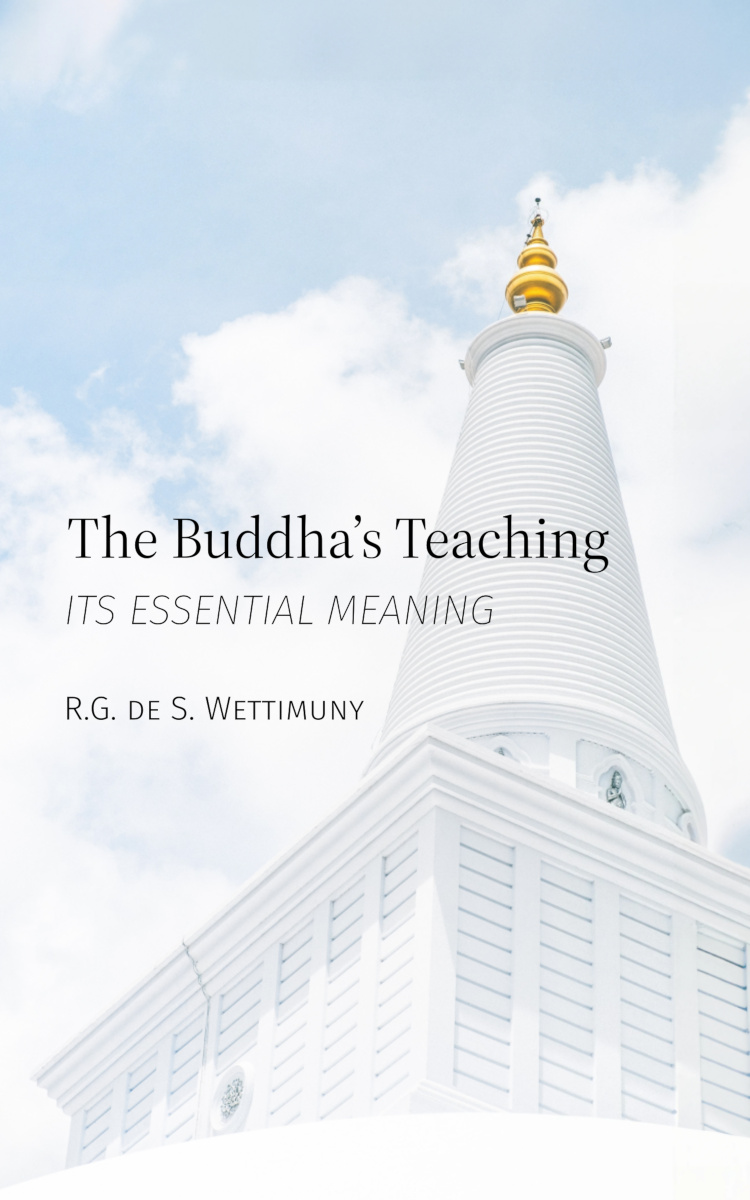
\includegraphics[height=\paperheight]{./desktop-cover.jpg}}
\fi

\cleartorecto
\thispagestyle{empty}
\vspace*{5em}

{\centering

\settowidth{\titleLength}{%
  {\Large\chapterTitleFont\scshape\MakeLowercase{\thetitle}}%
}

{\Large\chapterTitleFont\scshape\MakeLowercase{\thetitle}}\\[0.3\baselineskip]
\setlength{\xheight}{\heightof{X}}
\raisebox{0.5\xheight}{\color[gray]{0.4}\rule{\titleLength}{0.25pt}}\\[0.3\baselineskip]
{\itshape
\thesubtitle}

\vfill

\theauthor

\vspace*{5em}

}



\cleartoverso
\thispagestyle{empty}

{\copyrightsize
\centering
\setlength{\parindent}{0pt}%
\setlength{\parskip}{0.8\baselineskip}%

\thetitle\ -- \thesubtitle\\
by \theauthor

Published by \thePublisher

ISBN \theISBN

Copyright \copyright\ \thePublisher\ 2017

Cover Photograph: The Person

\vfill

{\footnotesize

This work is licensed under a Creative Commons\\
Attribution-NonCommercial-NoDerivatives 4.0 International~License.

Produced with the \LaTeX\ typesetting system, set in Gentium and Crimson Roman.

\theEditionInfo

}}


\cleartorecto
\tableofcontents*

\chapter{Preface}

In a letter to the author, the late Venerable Ñāṇavīra Thera stated:

\begin{quote}
\ldots{} unless one's thinking is all-of-a-piece, that is, properly speaking, no \authoremph{thinking} at all. A person who simply makes a collection -- however vast -- of ideas, and does not perceive that they are at variance with one another, has actually no ideas of his own, and if one attempts to instruct him (which is to say, to \authoremph{alter} him) one finds that one is adding to the junk-heap of assorted notions without having any other effect whatsoever. As Kierkegaard has said, `Only the truth that edifies is truth \authoremph{for you}.' Nothing that one can say to these collectors of ideas is truth \authoremph{for them}. What is wanted is a man who will argue a single point, and go on arguing it until the matter is clear to him, \authoremph{because he sees that everything else depends upon it}. With such a person communication (i.e. of truth that edifies) can take place.
\end{quote}

More so does the above apply when it comes to the Buddha's Teaching. In one's understanding of it, one must form an articulated, consistent, whole; a whole such that no one part can be modified without affecting the rest. At the outset it is not so important that the understanding is \authoremph{right}. That can \authoremph{only} come later. Nobody, after all, who has not reached the Path can afford to assume that he is right about the Buddha's Teaching.

With the Buddha's Teaching, however, if one's understanding of it is wrong, one will find that one cannot form a consistent whole. It then becomes the surest sign that some revision is necessary \authoremph{right down the line}.

In the \emph{Mūlapariyāya Sutta} (\emph{Majjhima Nikāya I}) the Buddha taught certain things as the fundamentals. Either these \authoremph{are} the fundamentals with regard to the problem of Suffering and its cessation, or the Buddha is wrong. It cannot be both. And if they \authoremph{are} the fundamentals, then there can be no hope of understanding his Teaching unless they are sufficiently appreciated. These fundamentals and their resultant implications are, however, difficult to \authoremph{see} though easy to state. They are beyond the scope of scholasticism. But they edify him who sees them. They are truth \authoremph{for him}.

There is always, however, the person to whom the Buddha's Teaching appears easy. But it appears easy only because he takes it up objectively and in conceptual fashion, and then passes it on; like the man who takes up a basket of mangoes, opens the lid, gazes at the mangoes, closes the lid, and passes the basket on. Taking up the Teaching in scholarly fashion, he thinks: What after all is there so difficult in understanding Impermanence, Not-self, and Suffering? As one breaks up the chariot into its constituent parts and finds there is nothing permanent or self-existent in it, he breaks up the personality (i.e. the Five Grasping Groups) into bits and pieces, these into further bits and pieces, and proclaims he cannot find any self in it anywhere. Therefore he thinks he perceives Not-self! The result is that he has very effectively called a halt to his own progress. In spite of all the masterly analysis of his personality into as many constituents as possible, and his finding no self-existent thing in it anywhere, he still looks upon his personality as `\authoremph{my self}'! He remains just where he started from, though he thinks he has advanced.

This `ease' of understanding only points to the shallowness of the understanding. What a decade ago, pursuing such scholasticism, appeared easy to the present writer -- that he now finds to be by no means easy. This however, not because his thinking powers have declined, but because the urge in him to \authoremph{see} a solution to the problem of his own existence has disquietingly brought out into the open those very same difficulties which in the earlier years he chose to treat rather lightly.

To what individual does the Buddha's Teaching matter? It matters to the individual who sees that the problem of his own existence is a \authoremph{present} problem, and wishes to have a solution to it \authoremph{in the present}. It is therefore only to such an individual that any book which endeavours to indicate what the Buddha taught can really matter.

R.G. de S. Wettimuny

40/13, Park Road, Colombo 5.\\
14.4.69

\clearpage

\section{A Note on the Translation of the Pali}

With regard to the translation of the Pali which is the language of the Buddhist Texts, the usual difficulty remains. That is, to produce a version which is both readable and accurate in meaning. To some extent readability has had to be sacrificed for the sake of accuracy in meaning. Hence the appearance of a few rather unusual phrases.

The Pali has been given alongside in many instances. This should assist the reader who has some knowledge of Pali. Actually one cannot come to understand the Buddha's Teaching without becoming familiar with the Pali.

{\raggedleft
R.G. de S.W.
\par}

\vspace*{3\baselineskip}

\begin{quote}
Formerly, and now also, Anurādha, it is just Suffering and the cessation of Suffering that I proclaim.

\emph{Pubbe cāham Anurādha etarahi ca dukkhañceva paññāpemi dukkhassa ca nirodhanti.}

 -- \href{https://suttacentral.net/sn44.2/en/sujato}{SN 44.2}, Anurādha Sutta
\end{quote}


% Page 1 is the first page of the first chapter.
\mainmatter

\chapter{Grasping}

\begin{quote}
``\,`Person! Person!' (\emph{sakkāya}), Venerable One, it is said. But what is it that the Exalted One has called the `person'?''

``These Five Grasping Groups (\emph{upādāna-kkhandhā}), friend Visākha, has the Exalted One called the `person', namely: the Grasping Group of Form, the Grasping Group of Feeling, the Grasping Group of Perception, the Grasping Group of Determinations, the Grasping Group of Consciousness. These Five Grasping Groups, friend Visākha, has the Exalted One called the `person'.''

 -- \href{https://suttacentral.net/mn44/en/sujato}{MN 44}, The Shorter Classification
\end{quote}

Thus the Buddha teaches me that I comprise five groups or aggregates of Grasping. The Pali word \emph{upādāna} has been translated here as \emph{Grasping}. It may also be translated as \emph{Holding}.

\begin{quote}
And what, monks, is Form (\emph{rūpa})? The Four Primary Modes (\emph{dhātu}), and the Form that is present by grasping (\emph{upādāya}) the Four Primary Modes -- this, monks, is called Form.

 -- \href{https://suttacentral.net/sn22.56/en/bodhi}{SN 22.56}, Perspectives
\end{quote}

The Four Primary Modes mentioned here are the Earth-Mode, Water-Mode, Fire-Mode and Air-Mode. They are often referred to as `elements'. But in relation to `matter', which is what Form refers to `elements' gives the idea of indivisible fundamental ingredients, and a wrong impression can be created that Buddhism splits the world-mass into four distinct fundamental ingredients. Form refers to what we call `matter'. But the Four Primary Modes do not refer to four elements or ingredients which constitute this `matter'. They refer to four distinguishable general \authoremph{modes of behaviour}, according to which `matter' makes itself known. The most important group of behaviours to me is that which I refer to as `my body' -- `this material body made up of the Four Primary Modes' (\emph{kāyo rūpī catummahābhūtiko}, \href{https://suttacentral.net/mn74/en/sujato}{MN 74}).

\begin{quote}
And what, monks, is Feeling (\emph{vedanā})? It is these six feeling-groups, namely: feeling sprung from Contact with the eye, feeling sprung from Contact with the ear, feeling sprung from Contact with the nose, feeling sprung from Contact with the tongue, feeling sprung from Contact with the body, feeling sprung from Contact with the mind. This, monks, is called Feeling.
\end{quote}

In the above passage, by Contact (\emph{phasso}) is not meant what is commonly referred to as `sense-impression'. As we shall see later on, Contact is the \authoremph{coming together} of three things, the sense-base (eye, ear, etc.), the corresponding percept (sight, sound, etc.), and the kind of Consciousness involved (eye-consciousness, ear-consciousness, etc.).

\begin{quote}
And what, monks, is Perception (\emph{saññā})? It is these six perception-groups namely: sight-perception, sound-perception, smell-perception, taste-perception, touch-perception, idea-perception (\emph{dhammasaññā}). This is called Perception.

And what, monks, are Determinations (\emph{sankhārā})? It is these six intention-groups (\emph{cetanākāya}), namely: intention with regard to sight, intention with regard to sound, intention with regard to smell, intention with regard to taste, intention with regard to touch, intention with regard to ideas. These, monks are called Determinations.

And what, monks, is Consciousness (\emph{viññāna})? It is these six consciousness-groups, namely: eye-consciousness, ear-consciousness, nose-consciousness, tongue-consciousness, body-consciousness, mind-consciousness. This, monks, is called Consciousness.

 -- \href{https://suttacentral.net/sn22.56/en/bodhi}{SN 22.56}, Phases of the Clinging Aggregates
\end{quote}

The personality is thus analysed and broken up into its constituent parts. My entire being is composed of them. Beyond them there is naught else for me. \authoremph{My world} is the totality of these Five Grasping Groups. They constitute \authoremph{my world}.

None of these Groups can however exist by itself separated from the others. They are inseparable, and of their inseparability the Venerable Sāriputta says:

\begin{quote}
Whatever, friend, there exists of Feeling, of Perception, and of Consciousness, these things are associated and not dissociated, and it is impossible to dissociate one from the other and show their differences. For, whatever one feels, one perceives and whatever one perceives, of that one is conscious.

 -- \href{https://suttacentral.net/mn43/en/sujato}{MN 43}, The Great Classification
\end{quote}

Then again we have the Buddha teaching:

\begin{quote}
Were one, monks, to declare thus: `Apart from Form, apart from Feeling, apart from Perception, apart from Determinations, I will show the coming, or the going, or the disappearance, or the appearance, or the growth, or the increase, or the abundance of Consciousness' -- that is not possible.

 -- \href{https://suttacentral.net/sn22.53/en/bodhi}{SN 22.53}, Engagement
\end{quote}

Before proceeding any further it is extremely important to understand clearly what the Buddha defines as Grasping (\emph{upādāna}), or as Holding.

The difference between life and inanimate things is that in the former there is \authoremph{intention}. All conscious action is \authoremph{intentional}, whilst action pertaining to inanimate things is devoid of intention.

Now, in the context of the Five Grasping Groups, the Buddha defines the Group of Determinations as the Group of Intention (\emph{cetanā}). But why does he describe it is a \authoremph{Grasping} Group? The rest of mankind has seen Intention as either good or bad intention, moral or immoral intention, and so on. Nevertheless the Buddha appears to see something far more fundamental and deep-rooted in it. All these intentions, whether they be good or bad, moral or immoral, or anything else, he groups together and describes as a Grasping. To him they all appear to be basically of one and the same character. They are all forms of Grasping.

What then is Grasping?

And what precisely is the difference between Grasping (\emph{upādāna}) and Intention (\emph{cetanā})?

This, more than any other, is the fundamental question posed by the Buddha's Teaching.

Now, it is easy to \authoremph{state} the answer, but it is extremely difficult to \authoremph{see} it.

The answer is: essentially, all notions of subjectivity, all notions of a `self' or a `person' or a `somebody', all thoughts of `I' and `mine', are Grasping. Thus the Grasping Group of Determinations (here Intention) means, the \authoremph{Group of Intention based an notions of `self' and thoughts of `I' and `mine'}. Intentions which are \authoremph{not} based on any notion of `self' or any thought of `I' or `mine' whatever are merely a Group of Intention.

We shall consider the relationship between the three notions: `self', `I' and `mine' in more detail later on. Of these three notions, the most fundamental one is `mine'. To \authoremph{grasp} something (or \authoremph{hold} something) means to \authoremph{consider it as `mine'}. It is not easy to \authoremph{see} this. But it is extremely important that it is seen.

To grasp Form means: to consider Form as `mine'. The Grasping Group of Form means \authoremph{Group of Form considered as `mine'}. So it is with the other Groups.

Further, if there be anything that is grasped or can be grasped, then that is the Five Groups or a part thereof. When I say I grasp a certain external material object, what I really mean is that I grasp those feelings, perceptions, etc., which arise when I become conscious of that object. If I do not want those particular feelings, perceptions etc., then I do not want the object also, and hence will not grasp it.

Now, just as much as one grasps Form, one grasps Feeling, Perception, Determinations and Consciousness also. One considers them all as `mine'.

My world is the Five Grasping Groups that go to make me up. If there is anything that I must comprehend, then it must be these.

\begin{quote}
Monks, I will show you things that are to be comprehended, and what comprehending is \ldots\hspace{0pt} Do ye listen to it. And what, monks, are the things to be comprehended? Form, monks, is a thing to be comprehended; Feeling is a thing to be comprehended; Perception is a thing to be comprehended; Determinations are a thing to be comprehended; Consciousness is a thing to be comprehended. These, monks, are the things to be comprehended. And what, monks, is comprehending \ldots\hspace{0pt}

 -- \href{https://suttacentral.net/sn22.106/en/sujato}{SN 22.106}, Should Be Completely Understood
\end{quote}

The immediate question that arises is: Could there be a Group of Form, a Group of Feeling, a Group of Perception, a Group of Determinations, a Group of Consciousness which is wholly and entirely \authoremph{devoid} of notions of `self' and thoughts of `I' and `mine'? Or, as against the Five Grasping Groups could there be just the Five Groups? Particularly, with regard to intentional action, could there be any such action which is \authoremph{unaccompanied} by any notions of `self' and thoughts of `I' and `mine'?

For the present we leave this question unanswered and proceed.

In the elucidation of the Five Grasping Groups, Consciousness takes the
pride of place. The reason for that is that any \textbf{experience} means
\textbf{being conscious of one or more of the other four Groups}. I am
conscious of Form (i.e. I am conscious either of my body or of an
external object or of both); I am conscious of Feeling; I am conscious
of Perception; and I am conscious of Determinations.


\begin{quotation}
"It is as with the
choir-master of a five-member choir who himself, as the chief, takes up
his part and in the performance of the whole piece takes in himself
along with it."


\end{quotation}

What now is Consciousness (\emph{viññāna})?


When I say I am conscious of something it means that that something is
\textbf{present} to me. A sight, a sound, a smell, a taste, a touch, or an idea
is present. I am \textbf{aware} of a certain perception, or the perception is
\textbf{present} to me. I am conscious of it.


Sometimes Consciousness is seen equated to the subject to whom the
phenomenon is present. This is not correct. Consciousness does not refer
to the subject. Neither does it refer to the phenomenon nor to a part of
the phenomenon. It is not \textbf{what} is present or a part of what is
present. It is only the \textbf{presence} of the phenomenon. It is the presence
of that which is present. A feeling is present to me. Consciousness is
not the feeling. It is only the presence of the feeling. It is the being
conscious of the feeling Presence that is 'mine' or presence 'for me' is
Grasping-Consciousness (\emph{upādāna-viññāna}).


Without sufficient reason, the Buddha says, no Consciousness arises.


\begin{quotation}
"Consciousness, monks, is named after that in dependence on which it
comes into being.


\begin{itemize}

\item The Consciousness which comes into being in respect of sights in dependence on the eye is called eye-consciousness;

\item the Consciousness which comes into being in respect of sounds in dependence on the ear is called ear-consciousness;

\item the Consciousness which comes into being in respect of odours in dependence on the nose is called nose-consciousness;

\item the Consciousness which comes into being in respect of tastes in dependence on the tongue is called tongue-consciousness;

\item the Consciousness which comes into being in respect of touch in dependence on the body is called body-consciousness;

\item the Consciousness which comes into being in respect of ideas in dependence on the mind is called mind-consciousness."

\end{itemize}


"Just as, monks, fire is named after that independence on which it
burns. The fire that burns in dependence on logs of wood is called a
log-fire; the fire that burns in dependence on chips is called a
chip-fire; the fire that burns in dependence on grass is called a
grass-fire; the fire that burns in dependence on cow-dung is called a
cow-dung fire; the fire that burns in dependence on husks is called a
husk-fire; the fire that burns in dependence on rubbish is called a
rubbish-fire. In the same way, monks, Consciousness is named after that
in dependence on which it comes into being. The Consciousness that comes
into being in respect of sights in dependence on the eye is called
eye-consciousness …"


 — \href{https://suttacentral.net/mn38/en/bodhi}{MN 38}, The Greater Discourse on the Destruction of Craving


\end{quotation}

The four Groups, Form, Feeling, Perception, Determinations, are called
the supports, or the footholds, or the base, for Consciousness.


\begin{quotation}
"There are these five kinds of seed, monks. What five? Seed from root,
seed from trunk, seed from joints, seed from shoots, and seed from
grain.


"If, monks, these five kinds of seed were present undamaged, not rotten,
unspoiled by wind and heat, capable of sprouting, well preserved, but
there is no earth and water, would, monks, these five kinds of seed come
to growth, spread, and increase?"


"No, Lord."


"If, monks, these five kinds of seed were damaged, rotten, spoilt by
wind and heat, incapable of sprouting, not well preserved, but there is
earth and water, would, monks, these five kinds of seed come to growth,
spread, and increase?"


"No, Lord."


"If, monks, these five kinds of seed were undamaged, not rotten,
unspoiled by wind and heat, capable of sprouting, well preserved, and
there is earth and water, would, monks, these five kinds of seed come to
growth, spread and increase?"


"Yes, Lord."


"As the earth, monks, should the four supports for the persistence of
Consciousness be regarded. As the water, monks, should delight and
attachment be regarded. As the five kinds of seed, monks, should the
nutritive Consciousness be regarded.


"If Consciousness persists, monks, it is by holding to Form that it
persists. With Form as object, with Form as support, in association with
delight, it attains to growth, spread and increase.


"If Consciousness persists, monks, it is by holding to Feeling …
Perception … Determinations … that it attains to growth, spread and
increase."


 — \href{https://suttacentral.net/sn22.54/en/bodhi}{SN 22.54}, Seeds


\end{quotation}

The footholds for Consciousness can be viewed from a second angle. That
is through a dual classification of \textbf{internal} and \textbf{external} bases. The
six sense-bases, viz., the eye, the ear, the nose, the tongue, the body,
and the mind, are called the internal bases or the internal supports for
Consciousness, whilst those phenomena corresponding to these six
sense-bases, viz., sight, sound, smell, taste, touch and idea are called
the external bases or the external supports for Consciousness. The
latter are called external bases because they are largely dependent on
objects external to the corresponding internal base.


Consciousness and the other four Groups Cannot therefore be comprehended
from a standpoint outside of them by any method of objective synthesis
induction, and so on. Through themselves, and only through themselves,
i.e., by one’s own experience \textbf{only} can they be understood.



\chapter{Name-and-Form and Consciousness}

When Consciousness is explained as something that arises and ceases, the question follows: What are the conditions necessary for the arising of Consciousness, and its ceasing?

To this, the Buddha gives the answer: Name-and-Form \emph{(nāma-rūpa)} is the basis, the genesis, the condition for Consciousness.

`What being present is Consciousness present? Dependent on what does Consciousness exist?' The answer is: `Name-and-Form being present, there is Consciousness. Dependent on Name-and-Form, Consciousness exists.' (\href{https://suttacentral.net/dn14/en/sujato}{DN 14})

Thus the condition necessary for the arising of Consciousness is Name-and-Form.

Again, `What being present is Name-and-Form present? Dependent on what does Name-and-Form exist?' The answer is: `Consciousness being present, there is Name-and-Form. Dependent on Consciousness, Name-and-Form exists.' (\href{https://suttacentral.net/dn14/en/sujato}{DN 14})

Thus the condition for Consciousness is Name-and-Form, and the condition for Name-and-Form is Consciousness.

\begin{quote}
Consciousness turns back from Name-and-Form; it goes not beyond.

 -- \href{https://suttacentral.net/dn14/en/sujato}{DN 14}, The Great Discourse on the Harvest of Deeds
\end{quote}

All this needs explaining.

To start with, there must be a clear understanding of what is referred to as Name-and-Form \emph{(nāma-rūpa)}. It is where there is no such understanding that one find this phenomenon called \emph{nāma-rūpa} referred to as `mind-and-matter'. \emph{Rūpa} is certainly `matter', but as we shall see \emph{nāma} is not `mind'.

Firstly, what is \emph{rūpa}, which has been translated as Form?

Form, as just stated, refers to `matter'.

Now, any Form or lump of `matter' can be regarded as a particular \authoremph{group of behaviours}. Since a particular lump of `matter' or a particular group of behaviours is always \authoremph{present} in the same fashion, I come to the \authoremph{conclusion} that that `matter' exists independent of my senses. Since I always note with regard to that `matter' the same sights, sounds, smells, etc. I conclude that that `matter' exists independent of myself. Further, since the same `matter' exhibits almost the very same sights, sounds, smells, etc. to every individual, we conclude that there is a `material world' existing quite independent of us individuals.

The various modes of behaviour are not dependent on Consciousness. But to distinguish one mode of behaviour from another they have to be \authoremph{cognized} or they must be made \authoremph{present}. When so cognized these behaviours \authoremph{appear} in a certain fashion, or, when they are made to be present they are then present in a certain fashion. That means, there is an \authoremph{appearance} of these behaviours (the word `appearance' being taken in a rather wide sense) -- an appearance which takes the form of sights, sounds, smells, etc. Further, this appearance behaves in a certain fashion. Thus there is both an \authoremph{appearance of behaviour} and a \authoremph{behaviour of appearance}. And the set of behaviours defining the particular lump of `matter' or object is \authoremph{inferred} from the behaviour of its \authoremph{appearance}.\footnote{See \href{ch-13-nibbana.xml\#the-four-primary}{Chapter 13, Nibbāna}: `But their {[}the Four Primary Modes} \authoremph{appearance} is a matter for Consciousness, and their `existence' is \authoremph{inferred} through the behaviour of this \authoremph{appearance}.'{]}

All modes of behaviour can be categorized under four main modes called the Four Primary Modes \emph{(catunnaṁ mahābhūtānaṁ)}. They are Earth-Mode, Water-Mode, Fire-Mode and Air-Mode. They may also be called the Solid-Mode, the Fluid-Mode, the Ripening-Mode and the Motion-Mode.

\begin{quote}
And what, monks, is the Earth-Mode \emph{(paṭhavīdhātu)}? The Earth-Mode may be internal, may be external. And what, monks, is the internal Earth-Mode? Whatever is hard, solid, is internal, \authoremph{grasped by oneself} (\emph{paccattaṁ \ldots{} upādinnaṁ}), that is to say: the hair of the head, the hair of the body, nails, teeth, skin, flesh, sinews, bones, marrow of the bones, kidneys, heart, liver, pleura, spleen, lungs, intestines, mesentery, stomach, excrement, or whatever other thing is hard, solid, is internal, grasped by oneself -- this, monks, is called the internal Earth-Mode. Whatever is the internal Earth-Mode and whatever is the external Earth-Mode, just these are the Earth-Mode \ldots{}

And what, monks, is the Water-Mode \emph{(āpodhātu)}? The Water-Mode may be internal, may be external. And what, monks, is the internal Water-Mode? Whatever is liquid, become liquid, is internal, grasped by oneself, that is to say: bile, phlegm, pus, blood, sweat, fat, tears, serum, saliva, mucus, synovial fluid, urine, or whatever other thing is liquid, become liquid, is internal, grasped by oneself -- this, monks, is called the internal Water-Mode. Whatever is the internal Water-Mode and whatever is the external Water-Mode, just these are the Water Mode \ldots{}

And what, monks, is the Fire-Mode \emph{(tejodhātu)}? The Fire-Mode may be internal, may be external. And what, monks, is the internal Fire-Mode? Whatever is heat, become heat, is internal, grasped by oneself, that is to say: that by which one is vitalized, that by which one is consumed, that by which one is scorched, that by which what has been munched, drunk, eaten and tasted is fully digested, or whatever other thing is heat, become heat, is internal, grasped by oneself -- this, monks, is called the internal Fire-Mode. Whatever is the internal Fire-Mode and whatever is the external Fire-Mode, just these are the Fire-Mode \ldots{}

And what, monks, is the Air-Mode \emph{(vāyodhātu)}? The Air-Mode may be internal, may be external. And what, monks, is the internal Air-Mode? Whatever is air, become airy, is internal, grasped by oneself, that is to say: winds going upwards, winds going downwards, winds in the abdomen, winds in the belly, winds permeating the limbs, in-breathing, out-breathing, or whatever other thing is air, become airy, is internal, grasped by oneself -- this, monks, is called the internal Air-Mode. Whatever is the internal Air-Mode and whatever is the external Air-Mode, just these are the Air-Mode \ldots{}

 -- \href{https://suttacentral.net/mn140/en/bodhi}{MN 140}, The Exposition of the Elements
\end{quote}

In the above definitions the Buddha refers to the Four Primary Modes as `grasped by oneself' \emph{(paccattaṁ upādinnaṁ)}. In other words, he is referring to the \authoremph{Grasping} Group of Form (to \emph{rūpa-upādāna-kkhandha}).

Beyond the above there is only one important thing (according to the Suttas) the Buddha has thought about Form: that is, the question of the Four Primary Modes `getting no footing' \emph{(na gādhati)}. We shall come to this later on. One might therefore wonder why the Buddha has taught so little about Form or `matter'. But the Buddha has a distinct purpose in his Teaching. And elucidations are made by him only in as far as such are necessary for that purpose. He seeks no intellectual approval of what he teaches. His Teaching is designed for a purpose. It is designed to lead one on \emph{(opanayika)} towards a particular goal.

The analysis of Form or `matter' given above is sufficient. No further analysis of it are essential, as they would not help me to solve the problem of the Five Grasping Groups, the problem of `my world'. What is essential is to realise that the analysis given by the Buddha is \authoremph{sufficient}.

Form, the Buddha teaches, indicates a certain characteristic. That is, the characteristic of persisting \emph{(paṭigha)}. It is similar to the idea of \authoremph{inertia} taught in physical science. A tendency for a body to \authoremph{maintain} its characteristics is demonstrated. By that what we really mean is: there is seen a tendency for the body to maintain its \authoremph{appearance}. This is a very important characteristic of Form. It is really because of this characteristic that we can distinguish various objects from one another. If the table does not remain the table and the book does not remain the book when I am continuing to be conscious of them I cannot then distinguish them from each other.

There is a material object.\footnote{`Material object' is not quite the same as `matter'. The former is a particular `lump of ``matter``\,'.} This object is \authoremph{not} dependent on Consciousness. But this object can be \authoremph{present} or \authoremph{not present}. Its presence is a matter of Consciousness. The object being present to the individual means that he is conscious of it. It has been `discovered' by his Consciousness as it were. Though the object does not depend on Consciousness there is no \authoremph{presence} of the object if there is no Consciousness. Consciousness means this \authoremph{presence}. \authoremph{I am conscious} of an object means that that object is \authoremph{present to me}.

Now, an object is always present in \authoremph{some fashion}. It is present \authoremph{as} shape, colour, smell, sound, etc. Its presence is therefore known by these. Or it is present in terms of these. Those things called shape, colour, sound, smell, etc., which are brought about when Consciousness `discovers' the object are called Name \emph{(nāma)}. It is as if the particular Name is \authoremph{how} the particular object is present (Consciousness). It is the \authoremph{appearance} of the object (the word `appearance' being again taken in a rather wide sense). Therefore, we can define Name \emph{(nāma)} as `how Form \emph{(rūpa)} is present \emph{(viññāna)}'. The \authoremph{how} or the \authoremph{manner} is Name, and the presence is Consciousness.

This appearance or `how it is present' is always given a designation \emph{(adhivacana)}. This designation therefore actually belongs to \emph{nāma}. But we refer to the object by this designation.

It must be noted that this `how it is present' includes a number of things. The shape, colour, smell, sound, etc., are the perceptions. Then there are certain feelings which are either pleasant, unpleasant or neutral. Further, there is Intention, Attention and Contact in relation to the object. All these go to make up Name \emph{(nāma)}. `Feeling, Perception, Intention, Contact, Attention -- this is called Name.' (\href{https://suttacentral.net/sn12.2/en/bodhi}{SN 12.2})

It should be quite clear from the above that \emph{nāma} is not `mind'. \emph{Rūpa} is `matter', but \emph{nāma} is not `mind'. `Mind', as a sense-base, is \emph{mano}; as mentality, it is \emph{citta}. Thus it is wrong to translate \emph{nāma-rūpa} as `mind-and-matter'.

It is not an uncommon thing to find Name \emph{(nāma)} being taken to include Consciousness \emph{(viññāna)}. This is wrong. Name does \authoremph{not} include Consciousness. It only entails Consciousness.

If we examine this further we shall find that:

\authoremph{(1.)} Since `matter' has the characteristic of inertia or persistence, its appearance is seen to persist or remain the same. That is since Form \emph{(rūpa)} has the characteristic of persistence \emph{(paṭigha)}, we discern in Name \emph{(nāma)} a persistence.

\authoremph{(2.)} Since appearance has some particular designation, its `substance' (i.e. the `matter' which gives this appearance) is seen to have a designation. That is, since Name \emph{(nāma)} has designation -- \emph{(adhivacana)}, we discern in Form \emph{(rūpa)} a designation.

It is important to see this since the Buddha refers to it when he teaches the relationship between Name-and-Form \emph{(nāmarūpa)} and Contact \emph{(phasso)}, a relationship which we shall presently come to. We shall then be taking a particular experience in order to make the matter more clear.

What now are Intention \emph{(cetanā)}, Attention \emph{(manasikāra)}, and Contact \emph{(phasso)} which are included in Name \emph{(nāma)}?

At this moment I am sitting. The \authoremph{present} phenomenon is a sitting position. This present phenomenon, the sitting position, now brings to mind certain other phenomena such as a standing position, a lying position, etc. From the present sitting position, which is now the actual, it is possible to \authoremph{make} actual one of these new positions or states which are now \authoremph{not present}. Thus there is one actual state and many possible ones.

There is a relation between the present sitting position and the possible standing position. Likewise, there is a relation between the present sitting position and the possible lying position. This relation in one case is \authoremph{that which is necessary to bring about the standing position from the sitting position}, and in the other case \authoremph{that which is necessary to bring about the lying position from the sitting position}. Both these relations are \authoremph{actions}. The \authoremph{type} of action varies slightly. But basically they are both \authoremph{actions}.

When the action is completed, and let us say, the standing position is present, then the sitting position has vanished, and the sitting position has become a \authoremph{possible} present. The present actual has disappeared giving way to a possible becoming the present actual. The disappeared actual present is now only a possible present.

Adopting the standing position involves \authoremph{selecting} or \authoremph{choosing} the standing position from all the possible positions. And so I \authoremph{exercise my choice}. There comes about an \authoremph{opted action}. Thus the action involved in the change from sitting to standing is the \authoremph{exercise of choice}. All other positions are sacrificed and this one position is consciously held to. This action, or this exercise of choice, is called \authoremph{Intentional Action}. From the intentional action there comes to be \authoremph{present} the new position. `Thus, Ānanda, intentional action is the field, Consciousness is the seed.'\footnote{\href{https://suttacentral.net/an3.76/en/thanissaro}{AN 3.76}, Continued Existence} Just as the seed springs up out of the field the new position becomes present (Consciousness) resulting from the intentional action \emph{(kamma)}.

\authoremph{All conscious action is intentional}. Conscious action is the exercise of preference for one available mode of behaviour or action at the expense of others. And it is this action, namely, the exercise of choice, that distinguishes life-action from material-action.

In the exercise of choice, or in intentional action, there is Attention \emph{(manasikāra)} towards that particular action. The attention on the action keeps the action going. The state of affairs is being preserved as it were. And intention cannot be present unless attention is present.

Contact \emph{(phasso)} now remains to be considered.

This word represents a very important phenomenon and so should be clearly understood. If this phenomenon called Contact is absent, there can be no experience. Examination of it also throws some light on how Name-and-Form is dependent on Consciousness and Consciousness is dependent on Name-and- Form.

\begin{quote}
In dependence on eye and sights springs up eye-consciousness. The \authoremph{coming together} of the three is called Contact \ldots{} In dependence on ear and sounds \ldots{} In dependence on nose and odours \ldots{} In dependence on tongue and taste \ldots{} In dependence on body and touch \ldots{} In dependence on mind and ideas springs up mind-consciousness. The \authoremph{coming together} of the three is called Contact.

 -- \href{https://suttacentral.net/sn12.43/en/bodhi}{SN 12.43}, Suffering
\end{quote}

There is something important to be noted here. Broadly, by Contact is meant the coming together of the percept, the sense-base and that particular sense-consciousness. But with regard to the \emph{puthujjana} (commoner)\footnote{\emph{Puthujjana} refers to the common or ordinary person, to the commoner.} what arises is Grasping-Consciousness \emph{(upādāna-viññāna)}. Therefore, with the \emph{puthujjana}, Contact is \authoremph{inclusive} of thoughts of `I' and `mine'. That is, there is contact between a subject who says `I' and `mine' and the object.

Contact \emph{(phasso)} is a particular form of coming together. It is a particular form of \authoremph{union}. Perception, Feeling and Determinations come about because there is such a coming together. In other words, Perception, Feeling and Determinations are dependent on Contact.

Yet, though Perception, Feeling and Determinations are dependent on Contact, Form is not dependent on Contact. Form is dependent on the Four Primary Modes.

\begin{quote}
\protect\hypertarget{dependent}{}{}Monk, it is to be seen that the Group of Form (or `matter') is dependent on the Four Primary Modes, is conditioned by the Four Primary Modes. The Group of Feeling is dependent on, is conditioned by Contact. The Group of Perception is dependent on, is conditioned by Contact. The Group of Determinations is dependent on, is conditioned by Contact.

 -- \href{https://suttacentral.net/mn109/en/sujato}{MN 109}, The Longer Discourse on the Full-Moon Night
\end{quote}

Now, Contact is dependent on Name-and-Form. The Buddha teaches that this should be understood thus:

\begin{quote}
``Ānanda, those modes, features, characteristics, exponents, by which Name-body is to be seen -- if all those modes, features, characteristics exponents, were absent would a coming together of designation be evident in the Form-body \emph{(rūpakāye adhivacanasamphasso)}?''

``It would not, Lord.''

``Ānanda, those modes, features, characteristics, exponents, by which Form-body is to be seen -- if all those modes, features, characteristics, exponents, were absent, would a coming together of inertia be evident in the Name-body \emph{(nāmakāye paṭighasamphasso)}?''

``It would not, Lord.''

``Ānanda, those modes, features, characteristics, exponents, by which Form-body and Name-body are to be seen -- if all those modes, features, characteristics, exponents, were absent, would a coming together of designation and a coming together of inertia be evident?''

``They would not, Lord.''

``Ānanda, those modes, features, characteristics, exponents, by which Name-and-Form is to be seen -- if all those modes, features, characteristics, exponents, were absent, would there be Contact (that particular coming together)?''

``There would not, Lord.''

``Ānanda, those modes, features, characteristics, exponents, by which Name-and-Form is to be seen -- if all those modes, features, characteristics, exponents, were absent, would there be Contact (that particular coming together)?''

``There would not, Lord.''

``Wherefore, Ānanda, just that is the reason, the ground the arising, the condition for Contact, to wit, Name-and-Form.''

 -- \href{https://suttacentral.net/dn15/en/bodhi}{DN 15}, The Great Discourse on Causation
\end{quote}

Since it is important to understand this rather difficult teaching let us analyse a particular experience to make it clear.

There is a bottle of ink, or I am conscious of a bottle of ink. That is the experience.

This means that a Form \emph{(rūpa)} which appears as a `bottle of ink' (Name, \emph{nāma}) is present (Consciousness, \emph{viññāna}).

Now, if Feeling, Perception, etc., were absent would there be present a `bottle of ink'?

This question expanded would run thus: If the black colour, the shape, the smell, the neutral feeling, the intention to dip the pen in it, etc., were absent would a designation `bottle of ink' pertain to that Form (to that lump of `matter')?

The shape, smell, etc., are the features of the Name-body, and `bottle of ink' is the \authoremph{designation}. Therefore, generalizing, the question would run thus: If those features, modes, characteristics exponents, by which the Name-body is discerned were absent, would there be a coming together of a designation in the Form-body?\footnote{`Designation in Form-body' \emph{(rūpakāye adhivacana)} corresponds to `appearance of behaviour'.}

The answer is: No.

Again, if the characteristics (like inertia) of the Form (of that lump of `matter') were absent, would the appearance designated `bottle of ink' remain so, or be inert?

Generalizing, the question would run thus: If those features, etc., by which Form-body is discerned were absent would there be a coming together of inertia in the Name-body?\footnote{`Inertia in Name-body' \emph{(nāmakāye paṭigha)} corresponds to `behaviour of appearance'.}

The answer is: No.

Thus, this particular coming together called Contact is possible only because Name has its own characteristics and Form has its own characteristics, which means that Contact is possible only because Name-and-Form are just what they are. Hence Contact is dependent on Name-and-Form.

That Consciousness is also dependent on Name-and-Form is now not so difficult to see. If Consciousness is to be there, Form must be there either as one's own or external to one; Intention must be there to determine what one should be conscious of; and, of course, where there is Intention there is Attention. But this alone is insufficient. Perception, Feeling, and Contact must also be there. Thus the sum total of Name-and-Form \authoremph{must} be present for Consciousness to be present. Hence Consciousness is dependent on Name-and-Form.

Earlier we saw that there must be Consciousness for Name-and-Form to be there, Name being the manner in which Form appears when one is conscious of it. Without Consciousness there can be no Name-and-Form. Thus we have the triad: Name-and-Form depends on Consciousness, Consciousness depends on Name-and-Form, and Contact depends on Name-and-Form.

Name-and-Form and Consciousness arise \authoremph{simultaneously}. One does not arise and wait for the other in time to arise in dependence upon it. They both arise in dependence on each other, and therefore \authoremph{together}. Likewise they cease together. If one is there, so is the other. There is a total-either-way-simultaneity.

There are things which, however, do not have a total-either-way-simultaneity as Name-and-Form and Consciousness have. For example perception and knowledge. `Perception arises first, knowledge arises thereafter (in dependence on Perception)' (\href{https://suttacentral.net/dn9/en/thanissaro}{DN 9}) But the case with Name-and-Form and Consciousness is different. Since they depend on each other they arise together and cease together. One neither precedes nor follows the other in time. The relationship that Name-and-Form and Consciousness bear towards each other is therefore one that is `not involving time' or `timeless' \emph{(akālika)}. As against this type of relationship, the relationship between in-breathing and out-breathing is one that is `involving time' \emph{(kālika)}, since one follows or precedes the other in time. Incidentally, \emph{akālika} is to be given no other meaning than the one just given, and it is important to note that this is the actual meaning of this word. Various other meanings seem to be given to this word, resulting in confusion particularly when it comes to the Doctrine of Dependent Arising \emph{(paṭicca-samuppāda)}.

The three Groups -- Feeling, Perception and Determinations -- taken together can also be called Name \emph{(nāma)}. Since Name has been defined as the totality of Feeling, Perception, Intention, Contact and Attention, it means that, in this context, Determinations is the totality of Intention, Contact and Attention. That is possible because Perception directly involves the pair of bases for Consciousness and the kind of Consciousness involved (e.g., eye, sights, and eye-consciousness), which means that Contact (which is the coming together of these -- three is included, and the Fourth Group Determinations (as Intention) includes Attention, since in the exercise of choice there is always attention on the particular thing chosen. Thus the Five Groups -- Form, Feeling, Perception, Determinations and Consciousness -- can also be called Name-and-Form and Consciousness.

\chapter{Taṇhā and Bhava}

We have seen that any actual present points to many possibilities. From these possibilities conscious life makes a choice and exercises it. In exercising the choice Consciousness finds its new footing.

The question now is: \textbf{What} determines that particular choice and no other? Why is it that at any given instant I choose to do this and not any other?

The answer is simply that I \textbf{want} that thing towards which \textbf{that} particular action will lead me. Keeping the wanted thing in mind, or wanting that thing, I take the action that will lead me to it. Of all the courses of action available I select and pursue that particular course of action which leads me to the wanted thing. Throughout the action, the wanting lasts.

Now, a \emph{puthujjana}'s want can be categorized under three main headings called \emph{kāma}, \emph{bhava} and \emph{vibhava}. Wanting any one or more of these things is called \emph{taṇhā}.

The word \emph{taṇhā} is usually translated as Craving or Thirst. This however, tends to give an inaccurate picture, since either of the words Craving or Thirst gives the impression of an acute wanting. But wanting \emph{kāma}, \emph{bhava} or \emph{vibhava} in the \textbf{slightest} degree is \emph{taṇhā}. On the other hand the word \textbf{wanting} is too wide to be used for \emph{taṇhā}, since though the Arahat has \textbf{no taṇhā} he certainly has other wants like wanting to eat food when hungry or wanting to rest when tired. There seems to be no exact English equivalent to \emph{taṇhā}, so we shall use it as it is.

The \emph{puthujjana} has \emph{kāma-taṇhā}, \emph{bhava-taṇhā} and \emph{vibhava-taṇhā}.

What now are \emph{kāma}, \emph{bhava} and \emph{vibhava}?

\emph{Kāma} is sense-pleasure,\footnote{Pleasure, it should be noted, is not the feeling born of the senses. One can take pleasure in a feeling or not take pleasure in it. Thus pleasure is a matter of one's mental attitude. The Buddha said that his mind was freed from the Taint of sense-pleasure (\emph{kāmāsavāpi cittaṁ vimuccitva}). Sight, sound, smell, taste and touch are the strands of sense-pleasure (\emph{kāmagunā}).} i.e., the pleasure connected with the senses. Wanting pleasure that arises in connection with one or more of the senses is called \emph{kāma-taṇhā}.

What is \emph{bhava}?

It is not possible to answer this question and indicate the meaning of the answer effectively and with sufficient clarity unless the question that was left unanswered in the first chapter is answered --- the question: As against the Five Grasping Groups could there be \textbf{just} the Five Groups?

The answer is: Yes.

The unique discovery that the Buddha made was just this: there could be Five Groups \textbf{without} Grasping. In other words, there could be an individual (i.e., as distinct from other individuals) who has no notion whatever of `self', `I' and `mine'. This individual is called Arahat (\emph{arahaṁ}). \textbf{The Arahat does not consider anything whatever as `mine'.} The Buddha experienced this state of affairs in himself. Thus he was the first Arahat to have appeared in the world in our time.

\textbf{Bhava} literally means `existence' or `being'. But existence of what? Being what? It refers to the \textbf{existence of `self'}, or to the notion \textbf{`I exist'}. Or we may say it refers to \textbf{being a `self'}, to \textbf{being a subject (`I')}. Or yet, to the \textbf{existence of subjectivity}. A life-mode completely devoid of all notions of `self' and of thoughts of `I' and `mine' will \textbf{not} be a \textbf{bhava}.

The \emph{puthujjana} looks upon his existence as `\textbf{my} existence'. He thinks `my self exists' or `I exist'. This looking upon one's existence as `my existence' or `existence of my self' is called having \emph{bhavadiṭṭhi}. When there are no notions of `self' no thoughts of `I' and `mine' there can be no such thing as `my existence' and so on.

To speak very precisely, \emph{bhava} is the existence of the notions `self' and `I'. Something is, of course, always identified as `self' and `I', which again, is one or more of the Five Grasping Groups. But \emph{bhava} is really a matter of one's thinking just as much as Grasping (\emph{upādāna}) is.\footnote{This should not lead the reader to think that since \emph{bhava} and \emph{upādāna} are really a matter of one's thinking they can be easily got rid of if necessary. If one completely gets rid of the thought `mine' so that it will never arise again, then one has become Arahat.}

It is the mind that is freed from the taint of \emph{bhava}, just as it is the mind that is freed from the taints of sense-pleasure and Ignorance. The Buddha said that his mind was freed from the taint of \emph{bhava}: `Thus knowing, thus seeing, my mind was freed from the taint of sense-pleasure, freed from the taint of \emph{bhava}, freed from the taint of Ignorance.' (\href{https://suttacentral.net/mn36/en/bodhi}{MN 36}) He described himself as `gone to the end of \emph{bhava}' --- \emph{bhavassa pāragu}. (\href{https://suttacentral.net/iti100/en/sujato}{Iti 100}) He did not say he was \textbf{going} to the end of \emph{bhava}. He said that he had already \textbf{gone} to the end of \emph{bhava}; which means he lives free from \emph{bhava}. In him \emph{bhava} has ceased. He is \emph{bhavanirodha}, because he is completely free from notions of `self' and from thoughts of `I' and `mine'. He does not look upon his existence as `\textbf{my} existence'. He does not think `\textbf{I} exist'. Certainly he uses the \textbf{words} `I' and `mine' for purposes of conversation. But that is all. They are expressions current in the world of which he makes use, but he is not at all affected by them.

The tendency to the conceit `I' and `mine' (\emph{ahaṅkāramamaṅkāramānānusaya}) is not always apparent, for it is not always on the surface. It lies deep-rooted and latent. It is something that one perceives only when one reflects upon it. One does not perceive it at all times even though it is present at all times lying behind one's thoughts and actions. In the Buddha, and in the Arahats, this tendency is completely uprooted, never to arise again. When all thoughts of `I' and `mine' are extinct and do not arise again, `my existence' or `I exist' are also extinct and do not arise again.

The Arahat `has gone beyond all \emph{bhava}' --- \emph{upaccagā sabbabhavāni}. (\href{https://suttacentral.net/ud3.10/en/sujato}{Uda 3.10}) The Arahat Maha Kassapa declared that he had `escaped from \emph{bhava}' --- \emph{bhavābhinissato}. (\href{https://suttacentral.net/thag18.1/en/sujato}{Thag 1089}) \emph{Bhava} ceases with the attainment of Arahatship. Thereafter the Arahat lives freed from \emph{bhava}, delivered from \emph{bhava}. Before the ascetic Gotama attained Arahatship all life that existed was \emph{bhava}. With his attaining Arahatship there came to be for the first time in the world a life free of \emph{bhava}.

\emph{Bhava} is also called a fetter. This fetter is completely cut off and destroyed in the Arahat. He is \emph{parikkhīnabhavasaññojano}. (\href{https://suttacentral.net/sn22.110/en/sujato}{SN 22.110})

If \emph{bhava} means `existence' pure and simple, then the living Arahat cannot have completely destroyed \emph{bhava}, for as a living Arahat there is an `existence'.\footnote{See \href{ch-08-impermanence.xml\#living-experience}{Chapter 8, Impermanence}: `The Not-Determined therefore is the \textbf{living experience of the Arahat}.'} The living Arahat has `existence', but no \emph{bhava}. He is \emph{bhava}-ceased. \emph{Bhava} refers to the existence of \textbf{all} modes of life \textbf{other than} that of the Arahats, simply because all such modes of life, save the Arahat's, are a case of `\textbf{my} existence' or `self'-existence to some degree or other.

If the precise meaning of \emph{bhava} is not understood there can be much confusion with regard to the Buddha's Teaching, particularly when it comes to the Doctrine of Dependent Arising (\emph{paṭiccasamuppāda}). The Teaching will then become either a matter of faith, which will remain beyond reach here, or a hypothesis left for future verification. But the Buddha's Teaching is neither a matter of faith nor a matter of hypothesis. It is a teaching to be experienced here and now, all of it, from beginning to end.

As with the word \emph{taṇhā}, there does not seem to be an exact equivalent in English for the word \emph{bhava}. This word is usually translated as `becoming' or `existence' --- all of which miss the point.\footnote{Sometimes \emph{bhava} is seen translated as rebirth! The extent to which the meaning of the Suttas (Discourses) is hidden from the reader by such inaccuracies can thus be seen.} We shall therefore keep to the Pali word \emph{bhava}.

Wanting \emph{bhava}, i.e., wanting `self'-existence or `my existence' is \emph{bhava-taṇhā}.

\emph{Vibhava} is not so straightforward as \emph{bhava}.

Some thinkers, in their search for truth, want to be quite certain of everything they take to be true. They begin by doubting everything, including their very existence. But by doubting their own existence they very cleverly deceive themselves for the simple reason that their very doubting proves their existence. To doubt also one must exist. \emph{Vibhava} stems out of this type of thinking. It is a denial of existence. Existence denies itself. But this denial of existence only leads to a confirmation of existence. It does \textbf{not} lead to \textbf{cessation} of existence.

Since, perhaps, it appears insane to deny existence whilst being existent, this tendency to denial is pushed back (\emph{atidhāvati}) to `after death', and in the following manner a denial of existence is made: `To the extent, revered Sir, that this self is of Form, is made up of the Four Primary Modes, is from the union of the parents, is cut off and destroyed on the dissolution of the body, and does not exist after death, to that extent is there a complete cutting off of the self.' (\href{https://suttacentral.net/dn1/en/bodhi}{DN 1})

This thinking, in the final analysis, only confirms `self'-existence. Thus \emph{vibhava} --- denial of `self'-existence --- only confirms \emph{bhava}, only confirms `self'-existence. It does not lead to \textbf{cessation} of `self'-existence. Just as \emph{bhava} is, \emph{vibhava} is also based on `self' and on thoughts of `I' and `mine'.

\begin{quote}
Those worthy recluses and brahmins who lay down for beings the cutting off, the destruction, the denial of \emph{bhava} (of `self'-existence), these, afraid of the `person' (\emph{sakkāya}), loathing the `person', simply keep running and circling round the `person'. Just as a dog that is tied by a leash to a strong post keeps running and circling round the post, so do these worthy recluses and brahmins, afraid of the `person', loathing the `person', simply keep running and circling round the `person'.

 --- \href{https://suttacentral.net/mn102/en/sujato}{MN 102}, The Five and Three
\end{quote}

Wanting the cutting off of `self'-existence and the destruction of `self'-existence at death is called \emph{vibhava-taṇhā}.\footnote{See \href{ch-99-appendix.xml\#vibhava-tanha}{Appendix on Vibhava-taṇhā}.} (It is an undesirability because such a destruction of `self'-existence cannot be got. `Self'-existence, or \emph{bhava}, can be destroyed only by following a particular training, i.e., by treading the Noble Eightfold Path.)

Just as much as grasping belief in `self' is the most fundamental of the four kinds of Grasping, wanting \emph{bhava} is the most fundamental of the three kinds of \emph{taṇhā}.

Thus the \emph{puthujjana}'s intentional action is determined by \emph{taṇhā}. `So, Ānanda, action is the field, Consciousness the seed, and \emph{taṇhā} the moisture.' (\href{https://suttacentral.net/an3.76/en/thanissaro}{AN 3.76}) Just as moisture must be present for the seed to sprout up out of the field, so must \emph{taṇhā} be there for the \emph{puthujjana}'s Consciousness to arise from his intentional action. \emph{Taṇhā} is one of the most powerful factors that go into the fashioning of one's life, yet it is one factor that can be brought under immediate control. The necessity to control \emph{taṇhā} cannot be overstressed if one is to progress. Hence the reason for the Buddha laying so much stress on it.

In the texts the words \emph{taṇhā}, \emph{chanda}, \emph{rāga} and \emph{nandi} often come together. There seems to be a tendency to consider the words \emph{chanda}, \emph{rāga} and \emph{nandi} as being almost identical with \emph{taṇhā}. They are not `various shades of \emph{taṇhā}'. They have their own meaning.

\emph{Chanda} means desire, \emph{rāga} means attachment, and \emph{nandi} means delight. Desire, attachment and delight are things dependent on \emph{taṇhā}. Were there no kind of wanting sense-pleasures or `self'-existence there can be no desire or attachment or delight.

\begin{quote}
Thus it is, Ānanda, that \emph{taṇhā} arises dependent on feeling, pursuit dependent on \emph{taṇhā}, gain dependent on pursuit decision dependent on gain, \textbf{desire} and \textbf{attachment} dependent on decision, tenacity dependent on desire and attachment, possession dependent on tenacity, avarice dependent on possession, watch and ward dependent on avarice, and many a bad and unskilled state of things such as blows and wounds, strife, contradiction and retort, quarrelling, slander and lies arise from keeping watch and ward.

 --- \href{https://suttacentral.net/dn15/en/bodhi}{DN 15}, The Great Discourse on Causation
\end{quote}

Desire (\emph{chanda}), attachment (\emph{rāga}) and delight (\emph{nandi}) have also been referred to as Grasping (\emph{upādāna}). `Friend, Visākha, that desire and attachment there is in the Five Grasping Groups, that there, is the Grasping.' (\href{https://suttacentral.net/mn44/en/sujato}{MN 44}) And, `Whatsoever there is delight in Feeling, that is Grasping.' (\href{https://suttacentral.net/mn38/en/bodhi}{MN 38}) This means to say that grasping something also means desiring of it, or being attached to it, or delighting in it. This is so because desiring, or being attached, or delighting, is \textbf{in effect} the same as regarding as `mine'. It is a matter of direct experience that when desire, attachment or delight exist `I' and `mine' also exist. It is only an `I' that can desire something or be attached to it or delight in it.

\emph{Taṇhā}, desire, attachment, delight, are all supports for \emph{bhava}. `\textbf{I} exist' or `\textbf{my} existence' stands supported by these. \emph{Bhava} hangs on these as its `cord'. They are called the `cord of \emph{bhava}' (\emph{bhavanetti}).

\begin{quote}
Whatever desire, attachment, delight, \emph{taṇhā}, whatever tendencies to determinations, attachments, and to the grasping of various means there are in the mind, Radha, towards Form \ldots{} Feeling \ldots{} Perception \ldots{} Determinations \ldots{} Consciousness, that is called the cord of \emph{bhava}. The cessation of these is the cessation of the cord of \emph{bhava}.

 --- \href{https://suttacentral.net/sn23.3/en/sujato}{SN 23.3}, The Conduit To Rebirth
\end{quote}

Just as a bunch of mangoes hanging by a stalk will fall down when the stalk is cut, so will \emph{bhava} disappear when the cord of \emph{bhava} is cut. The Buddha said that he stood with the cord of \emph{bhava} cut. Thus he stood freed from \emph{bhava}.

\begin{quote}
Just, monks, as when the stalk of a bunch of mangoes has been cut, all the mangoes that were hanging on that stalk go with it, just so, monks, the body of the Tathāgata stands with the cord that binds it to \emph{bhava} cut (\emph{ucchinnabhavanettiko}).

 --- \href{https://suttacentral.net/dn1/en/bodhi}{DN 1}, The All-embracing Net of Views
\end{quote}

\chapter{Kamma}

It is useful to discuss briefly the subject of intentional action once again.

\begin{quote}
Intention, monks, I declare is \emph{kamma}. Having intended, one does \emph{kamma} through body, speech, and mind.

 -- \href{https://suttacentral.net/an6.63/en/thanissaro}{AN 6.63}, A Penetrative Discourse
\end{quote}

This statement of the Buddha is not quite as simple as it is usually reckoned to be. Firstly, from the Sutta itself, it is clear that this statement was made in relation to the \authoremph{non}-Arahat. The literal meaning of \emph{kamma} is `action'. With the \emph{puthujjana} it therefore refers to `\authoremph{my} action' or `\authoremph{I} act'. The word \emph{kamma} is used in this sense. Further expanded, \emph{kamma} means `\authoremph{my} intentional action' or `the action \authoremph{I} intentionally take'. And \authoremph{all} action that is consciously done is intentional. This intentional action can be by means of body, speech, or mind.

Intentional action \authoremph{unaccompanied} by thoughts of `I' or `mine' is \authoremph{not kamma}. The Arahat has no thoughts of `I' and `mine'. Therefore the Arahat's intentional action is not \emph{kamma}. The Arahat has intentional action, but no \emph{kamma}. \authoremph{Kamma is the non-Arahat's intentional action.} Of the Arahat the Buddha says: `He does not commit new \emph{kamma}.'\footnote{Of all the many things about \emph{kamma} the Buddha has taught, such as the various types of \emph{kamma} and their various fruits \emph{(vipāka)}, this is the most important. It is also the most fundamental thing about it.}

Ethics is concerned with the question of `what should \authoremph{I} do'. Whether that `what should be done by \authoremph{me}' is good or bad, moral or immoral, etc., it is necessarily something which \authoremph{I} should do.

Ethics accepts that `I' and `mine' must exist. It builds itself on the basis that `I' is a necessity. Ethics may or may not be conscious of its own position here. Nevertheless that remains its basic position. Actually, ethics is a searching after the most comfortable or the best way in which `I' can exist. But, as we shall see later on, `I' exists only in so far as Ignorance of the Four Noble Truths exists. Ethics does not know this fact. Thus, in the final analysis, ethics is a searching after the most comfortable and best way in which Ignorance can exist. It is therefore no wonder that no two schools of ethics are in agreement. Wherever there is Ignorance, there is conflict.

Where `I' and `mine' are wholly and entirely extinct, there the question of what should \authoremph{I} do does not arise. Arahatship is \authoremph{the extinction of ethics} also. Whilst all religions, in the end, teach an ethics of some kind or other. Buddha teaches the extinction of \authoremph{all} ethics also.

The Buddha teaches the arising and ceasing of \emph{kamma} thus:

\begin{quote}
Monks, were there \emph{kamma} performed in lust, born of lust, conditioned by lust, arising from lust -- that \emph{kamma} is unskilful \emph{(akusala)}, that \emph{kamma} is blameworthy, that \emph{kamma} has pain as fruit, that \emph{kamma} leads to the arising of (further) \emph{kamma}. That \emph{kamma} does not lead to the cessation of \emph{kamma}. Monks, were there \emph{kamma} performed in hatred \ldots{} performed in delusion \ldots{} that \emph{kamma} is unskilful, that \emph{kamma} is blameworthy, that \emph{kamma} has pain as fruit, that \emph{kamma} leads to the arising of \emph{kamma}. That \emph{kamma} does not lead to the ceasing of \emph{kamma}. These, monks, are the three conditions for the arising of \emph{kamma}.

Monks, were there \emph{kamma} performed with non-lust, conditioned by non-lust, arising from non-lust -- that \emph{kamma} is skilful \emph{(kusala)}, that \emph{kamma} is praiseworthy, that \emph{kamma} has happiness as fruit, that \emph{kamma} leads to the ceasing of \emph{kamma}. That \emph{kamma} does not lead to the arising of \emph{kamma}. Monks, were there \emph{kamma} performed with non-hatred \ldots{} performed with non-delusion \ldots{} that \emph{kamma} is skilful, that \emph{kamma} is praiseworthy, that \emph{kamma} has happiness as fruit, that \emph{kamma} leads to the ceasing of \emph{kamma}. That \emph{kamma} does not lead to the arising of \emph{kamma}. These, monks, are the three conditions for the ceasing of \emph{kamma}.

 -- \href{https://suttacentral.net/an3.111/en/sujato}{AN 3.111}, Sources (1st)
\end{quote}

Summarized, the above means: unskilful \emph{kamma} leads to the arising of \emph{kamma}, and skilful \emph{kamma} leads to the cessation of \emph{kamma}. Or, unskilful intentional action accompanied by thoughts of `I' and `mine' leads to further intentional action accompanied by thoughts of `I' and `mine', and skilful intentional action accompanied by thoughts of `I' and `mine' leads to the cessation of intentional action accompanied by thoughts of `I' and `mine'. The Arahat not having any thoughts of `I' and `mine' whatsoever does \authoremph{not} perform \authoremph{either} skilful \authoremph{or} unskilful \emph{kamma}.

The Buddha further teaches how \emph{kamma} rooted in lust, hatred and delusion leads to further \emph{kamma} whilst \emph{kamma} rooted in non-lust, non-hatred and non-delusion leads to the cessation of \emph{kamma}, thus:

\begin{quote}
Monks, there are these three conditions for the arising of \emph{kamma}. What three? Monks, for things which in the past were based on desire and attachment \ldots{} in the future will be based on desire and attachment \ldots{} in the present are based on desire and attachment, desire is born.

How, monks, is desire born for things which in the past were based on desire and attachment \ldots{} in the future will be based on desire and attachment \ldots{} in the present are based on desire and attachment? Monks, things which in the past \ldots{} in the future \ldots{} in the present are based on desire and attachment, one turns over in his mind. Thus turning over in his mind things which in the present are based on desire, desire is born. Desire being born, he is fettered by those things. I call it a fetter, monks -- that mind full of attachment. Thus, monks, is desire born for things which in the present are based on desire and attachment. These are the three conditions, monks, for the arising of \emph{kamma}.
\end{quote}

On the other hand:

\begin{quote}
How, monks, is desire not born for things which in the past were based on desire and attachment \ldots{} in the future will be based on desire and attachment \ldots{} in the present are based on desire and attachment? Monks, one understands the future result of things which in the present are based on desire. Seeing this result one turns away from them. Turning away from them, the mind getting detached from them, one penetrates them with wisdom and sees them plain. Thus, monks, is desire not born for those things which in the present are based on desire.

 -- \href{https://suttacentral.net/an3.112/en/sujato}{AN 3.112}, Sources (2nd)
\end{quote}

It is now necessary to discuss the key-word \emph{saṅkhāra}, examine how it
appears in the various contexts, and determine whether a meaning to this
word which will comfortably accommodate all its applications could be
derived.


Below are six important uses of this word found in the Suttas:


Firstly, it is the name given to the fourth Group
(\emph{saṅkhāra-kkhandha}) which has been translated as the Group of
Determinations. This fourth Group is defined as \emph{cetanā-kāya}, i.e.,
as intention-group. Thus, in the context of the fourth Group, \emph{saṅkhāra}
is synonymous with intention (\emph{cetanā}).


Secondly, in the context of the Doctrine of Dependent Arising
(\emph{paṭiccasamuppāda}) where it occurs in \emph{saṅkhārapaccayā viññānaṁ},
it is defined as bodily-\emph{saṅkhāra}, verbal-\emph{saṅkhāra} and
mental-\emph{saṅkhāra} thus:


\begin{quotation}
"What, monks, are the \emph{saṅkhāra}? They are
the three \emph{saṅkhāra}, namely, bodily-\emph{saṅkhāra}, verbal-\emph{saṅkhāra}
and mental-\emph{saṅkhāra}. These, monks, are called the
\emph{saṅkhāra}."


 — \href{https://suttacentral.net/sn12.2/en/bodhi}{SN 12.2}, Analysis of Dependent Origination


\end{quotation}

These three kinds of \emph{saṅkhāra} are in turn defined in the
\emph{Cūlavedalla Sutta}  as follows:


\begin{quotation}
"Friend, Visākha, in-breathing and out-breathing are the
bodily-\emph{saṅkhāra}. Discursive thinking is the verbal-\emph{saṅkhāra}
Perception and Feeling are the mental-\emph{saṅkhāra}."


"Noble lady, for what reason are in-breathing and out- breathing the
bodily-\emph{saṅkhāra}? For what reason is discursive thinking the
verbal-\emph{saṅkhāra}? For what reason are Perception and Feeling the
mental-\emph{saṅkhāra}?"


"Friend, Visākha, in-breathing and out-breathing are corporeal. These
are \textbf{closely connected with} (\emph{paṭibaddhā}) the body. Therefore they are
bodily-\emph{saṅkhāra}. Having earlier had discursive thinking, one
subsequently utters words. Therefore discursive thinking is
verbal-\emph{saṅkhāra}. Perception and Feeling are mental. These are
closely connected with the mind. Therefore they are mental-\emph{saṅkhāra}."


 — \href{https://suttacentral.net/mn44/en/sujato}{MN 44}, The Shorter Classification


\end{quotation}

Thirdly, in the \emph{Kukkuravatiya Sutta}, bodily-\emph{saṅkhāra},
verbal-\emph{saṅkhāra} and mental-\emph{saṅkhāra} appear in a somewhat different
context thus:


\begin{quotation}
"Here, Punna, someone determines a
bodily-\emph{saṅkhāra} that is harmful, determines a verbal-\emph{saṅkhāra}
that is harmfu1, determines a mental-\emph{saṅkhāra} that is harmful. He
having determined a bodily-\emph{saṅkhāra} … a verbal-\emph{saṅkhāra} … a
mental-\emph{saṅkhāra} that is harmful, upbrings a world that is harmful."


 — \href{https://suttacentral.net/mn57/en/bodhi}{MN 57}, The Dog-Duty Ascetic


\end{quotation}

Fourthly, in the context of the Doctrine of Dependent Arising, the
\emph{Parivīmaṁsana Sutta} contains \emph{saṅkhāra} as
meritorious-\emph{saṅkhāra}, demeritorious-\emph{saṅkhāra}, and
imperturbable-\emph{saṅkhāra}, thus:


\begin{quotation}
"Were, monks, an ignorant individual
to determine a meritorious-\emph{saṅkhāra} his consciousness would go
towards merit. Were he to determine a demeritorious-\emph{saṅkhāra} his
consciousness would go towards demerit. Were he to determine an
imperturbable-\emph{saṅkhāra} his consciousness would go towards
imperturbability. A monk who has got rid of Ignorance and has attained
to Knowledge, monks, through such non-attachment to Ignorance and the
arising of Knowledge does not determine meritorious-\emph{saṅkhāra}, does
not determine demeritorious-\emph{saṅkhāra}, does not determine
imperturbable-\emph{saṅkhāra}. Not determining, not intending, he grasps at
nothing in the world."


 — \href{https://suttacentral.net/sn12.51/en/sujato}{SN 12.51}, Thorough Investigation


\end{quotation}

Fifthly, the \emph{Khajjaniya Sutta} identifies \emph{saṅkhāra} as the fourth Group thus.


\begin{quotation}
"Why, monks, do ye say \emph{sahkhāra}? They determine (\emph{abhisaṅkaronti})
the determined. That is why they are called \emph{saṅkhāra}. What is the
determined that they determine? Determined Form do they determine in
accordance with the nature of Form. Determined Feeling do they determine
in accordance with the nature of Feeling. Determined Perception do they
determine in accordance with the nature of Perception. Determined
Determinations do they determine in accordance with the nature of
Determinations. Determined Consciousness do they determine in accordance
with the nature of Consciousness. They determine the determined. That is
why they are called \emph{saṅkhāra}."


 — \href{https://suttacentral.net/sn22.79/en/bodhi}{SN 22.79}, Being Devoured


\end{quotation}

Sixthly, in the \emph{Mahāvedalla Sutta} (\href{https://suttacentral.net/mn43/en/sujato}{MN 43}) heat is called a life-\emph{saṅkhāra},
as that on which depends (\emph{paṭicca}) life.


It might assist the reader to see the above mentioned relationships
better if they are presented in the following manner:


FIXME: add figure.


Thus, firstly, \emph{saṅkhāra} is synonymous with intention as adopted in the
case of the fourth Group in the Five Groups. Secondly, in the
\emph{Cūlavedalla Sutta} we cannot equate \emph{saṅkhāra} entirely to intention.
Thirdly, the three kinds of \emph{saṅkhāra} mentioned in the \emph{Kukkuravatiya
Sutta} appear in the said Sutta as varieties of intentional action,
and therefore have a lot to do with intention. Fourthly, in the
\emph{Parivīmaṁsana Sutta}, \emph{saṅkhāra} are again certainly some kind of
intention upon which the Consciousness of the ignorant individual
depends. Fifthly, in the \emph{Khajjaniya Sutta}, \emph{saṅkhāra} (synonymous
with intention) are described as things that determine the Five Groups.
And, Sixthly, in the \emph{Mahāvedalla Sutta} life-\emph{saṅkhāra} is given as
heat upon which depends life.


Now, the words \emph{paṭibaddhā} in the \emph{Cūlavedalla Sutta} passage,
\emph{abhisaṅkaronti} in the \emph{Khajjaniya Sutta} passage, and \emph{paṭicca} in the
\emph{Mahāvedalla Sutta} passage are most indicative of what the word
\emph{saṅkhāra} means. It means:


\begin{itemize}

\item a thing to which some other thing is closely connected, or

\item a thing upon which some other thing depends, or

\item a thing without which some other thing cannot be, or

\item a thing which determines some other thing.

\end{itemize}


\emph{Saṅkhāra}, therefore, in short means: a determination,
or \textbf{necessary condition}. This one meaning covers all uses of this word.


What is meant by determination or \textbf{necessary condition} (that is to say,
\emph{saṅkhāra}) must be distinctly understood. It means that whatever
thing depends upon this necessary condition, that thing can exist \textbf{only if}
this necessary condition is present. The thing cannot be present
without the necessary condition being present. If the necessary
condition is absent, then the thing is also absent. It should not be
understood as 'once the necessary condition has come and gone the thing
arises'. Nor must it be understood as 'the necessary condition \textbf{becomes}
the thing'. No. There is no \textbf{temporal} succession one after the other. If
the necessary condition is gone, then the thing is also gone. This is a
\textbf{structural principle}.


It should also be clearly understood that \emph{saṅkhāra} do not refer to the
things (\emph{dhammā}) for which they form necessary condition. The things
that are determined or upbuilt with the \emph{saṅkhāra} as necessary
condition are called \emph{saṅkhatā dhammā} (determined things). These
\emph{saṅkhatā dhammā} are, however, \textbf{of the nature of saṅkhāra}. That is
to say, these determined things in turn act as the necessary condition
for other determined things.


For example, the Six Bases are necessary
condition for Contact. This means that Contact cannot come about without
the presence of the Six Bases. Thus, in this instance, the Six Bases are
\emph{saṅkhāra} and Contact is a \emph{saṅkhatā dhammā}. But again, Contact
which is on the one hand a \emph{saṅkhatā dhammā} is the necessary condition
for something else, viz., Feeling. Without Contact, no Feeling. Thus
Contact as a \emph{saṅkhatā dhammā} is also a \emph{saṅkhāra}, dependent upon
which stands Feeling.


The same applies to the Five Grasping Groups. The
Five Grasping Groups are \emph{saṅkhatā dhammā} with \emph{saṅkhāra} (primarily,
intention) as necessary condition. But they are also the necessary
condition for something else, viz., Grasping. Thus, the Five Grasping
Groups are both \emph{saṅkhatā dhammā} and \emph{saṅkhāra}. That is what is
meant by saying that all \emph{saṅkhatā dhammā} are in the nature of
\emph{saṅkhāra}.


These implications of the word \emph{saṅkhāra}, have to be clearly
understood. Quite a lot of the fanciful interpretations of the
Buddha-word are due to not understanding the precise meaning of the word
\emph{saṅkhāra} and the manner in which it is used in the Suttas.



With this we come to the problem of 'self'. It is in fact the basic problem. It is also more difficult a problem than it is generally supposed to be. And if one is speaking of the Buddha's Teaching then fundamentally one is speaking of \emph{attavādupādāna} (holding to belief in 'self') and \emph{asmimāna} (the conceit 'I am'). For, a Teaching that is meant to lead on to a cutting off at the root that which is called \emph{upādāna} must necessarily have a great deal to do with the most fundamental of \emph{upādāna}, viz., \emph{attavādupādāna}. The Buddha's Teaching sets out to destroy Suffering, and this, as we shall see later on, is to destroy and uproot beliefs in 'self' and thoughts of 'I' and 'mine', which again is to uproot \emph{upādāna}. "Uproot false view of seIf."\footnote{\href{https://suttacentral.net/snp5.15/en/sujato}{Snp 5.15}, The Question of Posāla} With the uprooting and destruction of these false views other things follow.

The notion of 'self-hood' is fundamentally a notion of \textbf{mastery}\footnote{The Pali word is \emph{vasa}. See \href{https://suttacentral.net/mn35/en/sujato}{MN 35}.} over things, a notion of being able to wield power over things, which in the final analysis is a notion of mastery over Form, Feeling, Perception, Determinations and Consciousness. 'I am master over this body, it is mine.' Or else, 'I am master over my intentions, they are mine.' To own or appropriate a thing means to become master over it, to wield power over it. Moreover, I think that 'I am' is something pleasant and pleasurable only when I feel or think I am permanently \textbf{master} over my Form, Feeling, Perception, Determinations and Consciousness, and I have \textbf{power} over them so as to make them become just what I want them to be. This feeling is the feeling of 'self-hood', and with it I lull myself into a false sense of security.

Though in times of right mindfulness the \emph{puthujjana} may tend towards seeing impermanence, the \emph{puthujjana}'s reaction towards things is as if they were permanent. His actions are based upon such wrong view. Basing himself on this wrong view he intends and acts. Whatever mastery he possesses is very \textbf{temporary} and very \textbf{partial}. Impermanence undermines the mastery. And a mastery that is undermined by impermanence is certainly no mastery. In short, the assumed 'self-hood' is no 'self- hood' at all. 'Self-hood' is therefore a \textbf{deception}.

I really do not wield power or possess mastery over the Five Grasping Groups which I regard as \textbf{my own}. I cannot say to my Consciousness: "Let my Consciousness be thus, let my Consciousness be not thus." I cannot say to my body which is suffering from an ulcer, "Let my body be relieved of the ulcer" and so have my body relieved of the ulcer. I certainly wish that from this body which I regard as my own the ulcer would vanish. In fact I think that it should never have come at all. But however much I wish the ulcer to vanish it does not. Nor can I wield any such power over the other Groups which I regard as 'mine'. I cannot say to the feelings which I regard as 'mine', "Let my feelings be thus, let my feelings be not thus", and so have my feelings as I want them to be. Thus this 'self-hood' which is adhered to is a deception, ever and again leading to betrayal, to disappointment. Betrayal and disappointment are the inevitable outcome of adhering to a deception.

Now, the \emph{puthujjana} has \emph{attavādupādāna}. That is to say, the \emph{puthujjana} holds (\emph{upādāna}) to belief (\emph{vāda}) in 'self' (\emph{attā}).\footnote{"Holding to belief in 'self'" essentially means holding to belief in a master.} Because he holds to this belief in 'self' he keeps looking for something which he can \textbf{identify} as this his 'self'.\footnote{To "identify something as his 'self'" essentially means to identify something as that thing over which he is master.} If he is to keep believing there is a 'self' then he \textbf{must} at the same time regard something or other as this 'self'. And if there is anything that he is led to identify as this his 'self' it must pertain to the Five Grasping Groups. It must be one or more of these Groups. It is impossible for him to identify it with anything else. He therefore views one or more of the Groups as 'self'.\footnote{To view the Groups as 'self' essentially means to regard that 'I am master over the Groups'. 'The Groups are my self' means 'I am master over my Groups'.} This means he has gone to wrong view. He has gone to the wrong view that one or more of his Groups is 'self'. Having thus gone to a wrong view he elaborates on the view and formulates a distinction between himself and the rest thus: 'The self, the world' (\emph{attā ca loko ca}). And he further keeps deliberating about himself (that is about the Five Grasping Groups regarded as 'self') thus:

\begin{quote}
\begin{itemize}
\item
  'Was I in the past',
\item
  'was I not in the past',
\item
  'who was I in the past',
\item
  'how was I in the past',
\item
  'having been who in the past who have I come to be now',
\item
  'will I be in the future',
\item
  'will I not be in the future',
\item
  'who will I be in the future',
\item
  'how will I be in the future',
\item
  'being who in the future whom will I be again in the future'.
\end{itemize}

About his present existence too he begins to doubt:

\begin{itemize}
\item
  'Am I',
\item
  'am I not',
\item
  'who am I',
\item
  'how am I',
\item
  'from where has this being come',
\item
  'where is he going'.
\end{itemize}

Further, one or other of the following views arises in him as though it were real and true:

\begin{itemize}
\item
  'There is self for me',
\item
  'there is not self for me',
\item
  'by self I recognize self',
\item
  'by self I recognize not-self',
\item
  'by not-self I recognize self',
\item
  or 'this my self which feels pleasant and unpleasant feelings, reaps the fruit of good and bad action, is permanent, steadfast, eternal, not transitory, stands unchanging as an eternal thing'.
\end{itemize}

 --- \href{https://suttacentral.net/mn2/en/bodhi}{MN 2}, All the Taints
\end{quote}

Thus he is gone to (wrong) view, or he is of (wrong) view (\emph{diṭṭhigata}).

All this deliberating about 'self' is because he is attached to a belief in 'self', because he has desire and passion towards 'self'. If he does not hold to a belief in 'self', these deliberations do not arise.

This regarding or viewing the Grasping Groups as 'self' in some way or other is called the 'person'-view (\emph{sakkāyadiṭṭhi}).

\begin{quote}
"But how, noble lady, is there the 'person'-view?"

"Here, friend Visākha, the uninstructed \emph{puthujjana} not discerning the Noble Ones, not skilled in the Noble Doctrine, untrained in the Noble Doctrine, not discerning the Worthy Ones, not skilled in the Doctrine of the Worthy Ones, untrained in the Doctrine of the Worthy Ones, regards

\begin{itemize}
\item
  Form \ldots{} Feeling \ldots{} Perception \ldots{} Determinations \ldots{} Consciousness as 'self',
\item
  or regards 'self' as having Consciousness,
\item
  or regards Consciousness as being in 'self',
\item
  or regards 'self' as being in Consciousness.
\end{itemize}

Thus, friend Visākha, it is said there is the 'person'-view."

 --- \href{https://suttacentral.net/mn44/en/sujato}{MN 44}, The Shorter Classification
\end{quote}

But why say '\textbf{person}'-view (\emph{sakkāyadiṭṭhi})?

\emph{Sakkāya} means 'person', 'somebody', a 'self-existing being'.\footnote{It does not matter very much what word we use as the English equivalent of the Pali word \emph{sakkāya}. The fact is that whatever word we use to denote \emph{sakkāya} will equally baffle the individual who does not understand its meaning. What is needed is not so much a precise English equivalent for the word \emph{sakkāya} as much as understanding what it refers to.} To the \emph{puthujjana} he is himself a \emph{sakkāya}, i.e., a 'person', a 'somebody', a collection of Five Grasping Groups which regards itself as master over itself. To be precise the Five Grasping Groups takes itself to be a \emph{sakkāya}.

Another word is \emph{satta}. The \emph{puthujjana} takes himself to be a \emph{satta}. \emph{Satta} or \emph{sakkāya} refers to the sentient being regarded in some way or other as 'self'. That is, it refers to the Five Grasping Groups taken to be 'self'. It is the \emph{puthujjana}'s concept of the sentient being. It is his concept of himself. That is why the Five Grasping Groups are called \emph{sakkāya}.\footnote{"What, monks, is the \emph{sakkāya}? The Five Grasping Groups are to be so called." (\href{https://suttacentral.net/sn22.105/en/sujato}{SN 22.105})} To have this concept means to be gone to 'person'-view.

Again, the Five Grasping Groups looks upon itself as 'self' so long as it contains \emph{attavādupādāna}, i.e., so long as it holds to belief in 'self'. \emph{Sakkāya} incorporates \emph{sakkāya-diṭṭhi}; that is to say, 'person' contains 'person'-view.\footnote{This statement is not fully applicable to the \emph{sotāpanna}, and higher \emph{sekhas}. To the extent that thoughts of 'I' and 'mine' and the deception 'self' arise in them, they are still \emph{sakkāya}. But they know that regarding anything as 'I am' or as 'mine' or as 'self' is wrong. Therefore they do not hold to any belief in 'self'. Thus they have no \emph{attavādupādāna}, and to that extent have no \emph{sakkāyadiṭṭhi} also. See also \href{ch-16-satipatthana.xml\#truth-for-him}{Chapter 16, Four Applications of Mindfulness}: "The \emph{Satipatthānā Sutta} assumes a prior understanding of the Buddha's Teaching. {[}\ldots\hspace{0pt}} though these fundamentals and their resultant implications are very difficult to \textbf{see}, they edify him who sees them. They are truth \textbf{for him}."{]} It should be noted that \emph{sakkāyadiṭṭhi} is not a question of just passively viewing oneself as a \emph{sakkāya} in a rather detached manner. It is much more dynamic and intense a matter, deeply rooted. Hence the difficulty in getting rid of it.

\emph{Sakkāyadiṭṭhi} should not be identified purely and simply with "the view that \textbf{in} the Five Grasping Groups there is a self" or with "the belief in a self or soul". Regarding one or more of the Five Grasping Groups as 'self' in some way or other is different to purely and simply regarding the Five Grasping Groups as having a 'self' \textbf{in} them somewhere or other. The person who mistakes \emph{sakkāyadiṭṭhi} to mean purely and simply "the view that in the Five Grasping Groups there is a self" can very effectively impede his own progress and even think he is an \emph{ariya} (Noble One) whilst he is not.

After a masterly analysis of the Five Grasping Groups, perhaps with the assistance of modern science, he finds no self-existing thing in it. Thus quite honestly he comes to the conclusion that there is no self in the Five Grasping Groups, and so he thinks he has no \emph{sakkāyadiṭṭhi}, which means he now thinks he is a \emph{sotāpanna},\footnote{See Chapter XV for definition of the \emph{sotāpanna}. At this stage it would be sufficient to know that the \emph{sotāpanna} is not a \emph{puthujjana} and that he is therefore an \emph{ariya}, i.e. he is a Noble.} whilst in truth he really is not.

The Five Grasping Groups constantly recognizes itself as 'self'. It is its very nature. And the apparent 'self', or that which appears as 'self' is taken as it appears and is identified as 'self'.

\emph{Sakkāyadiṭṭhi} is a determined thing (\emph{saṅkhata dhamma}), because it has come about with \emph{attavādupādāna} as necessary condition. Here, \emph{attavādupādana} is a \emph{saṅkhāra}. As a \emph{saṅkhāra} it is the necessary condition for \emph{sakkāyadiṭṭhi}. Without \emph{attavādupādāna} there can be no \emph{sakkāyadiṭṭhi}. Because the \emph{puthujjana} holds to belief in 'self' he views the Five Grasping Groups (or one or more of them) as this 'self' which he believes in.

On the other hand, if there is no holding to belief in 'self', then there can be no \emph{sakkāyadiṭṭhi}, because then no identification or regarding of anything as 'self' will arise. The \emph{puthujjana} does not see this. He does not see that his \emph{sakkāyadiṭṭhi} is dependent on a \emph{saṅkhāra} and that all \emph{saṅkhāras} are \textbf{impermanent}. But if he sees that the \emph{saṅkhāra} called holding to belief in 'self' (\emph{attavādupādāna}) is impermanent then the \emph{saṅkhāra} will cease, and he will no longer be deceived into believing in any 'self'. When \emph{attavādupādāna} ceases his identification of the sentient being as self ceases, which means \emph{sakkāyadiṭṭhi} ceases and he ceases to be a \emph{puthujjana}. He has then crossed from the plane of the \emph{puthujjana} (\emph{puthujjana bhūmi}) to the plane of the Noble (\emph{ariya bhūmi}).

Of the three notions 'This is mine, this am I, this is my self', the most fundamental one is '\textbf{this is mine}'. In the Discourse on \emph{The Fundamentals of All Things} (Majjhima Nikāya 1) the Buddha narrates at length the many things that the \emph{puthujjana} takes to be 'mine'. He does \textbf{not} include the other two notions of 'I' and 'self' at all in this Discourse.

Further, in the \emph{Ānanda Sutta} we have the following:

\begin{quote}
"By grasping Form is there 'I am', not by not-grasping (\emph{rūpam upādāya asmīti hoti no anupādāya}). By grasping Feeling \ldots{} Perception \ldots{} Determinations \ldots{} Consciousness is there 'I am', not by not-grasping."

 --- \href{https://suttacentral.net/sn22.83/en/bodhi}{SN 22.83}, Ānanda
\end{quote}

This too indicates that 'mine' (which is essentially the same as what has been referred to in the Sutta as grasping) is more fundamental than 'I', and that for 'I' to be present 'mine' must be present.

It is of great \textbf{practical} importance to see that 'mine' is the most fundamental of these three notions 'mine', 'I' and 'self'. The \emph{puthujjana}'s constant thinking is a thinking that something is \textbf{his}. In fact there is nothing more fundamental than this about his experience. And he must seek to understand this state of affairs in his own experience itself. The notions 'I' and 'self' do not take the same stature as the notion 'mine'. When he, the \emph{puthujjana}, is conscious of a feeling, he is always conscious of it as \textbf{my} feeling. It is this consideration 'mine' that leads the \emph{puthujjana} on.

The \emph{puthujjana}, however, works with the assumption that the fundamental is 'I' and not 'mine'. Since \textbf{he} exists, he thinks things are \textbf{his}. "\textbf{Since 'I'} exist, things are \textbf{mine}." But the fundamental condition, the Buddha points out, is 'mine'. The \emph{puthujjana} having Grasping Consciousness, things \textbf{present} themselves to him as \textbf{'mine'}. And this state of affairs further \textbf{points} to a subject to \textbf{whom} they are present. That is, they point to an 'I'. The correct position is therefore: \textbf{Since things are 'mine', 'I' exist.}

The \emph{puthujjana} then begins to wonder what precisely this 'I' is. He begins to reflect upon the 'I'. And when he so reflects he sees a 'self'; that is to say, he sees a mastery over things. A 'self' appears before him as he reflects, just as 'water' appears to the deer when it gazes upon the sun shining on the sand. 'Mine' being present all the time, this 'self' also appears as '\textbf{my} self'.

Finally, the \emph{puthujjana} --- holding to belief in 'self' all the time --- tries to identify this 'self'. But he can identify it with nothing else other than one or more of the Five Grasping Groups. He therefore proceeds to regard or view one or more of the Groups as 'self' --- more precisely, as 'my self'. He thinks 'The Groups are myself', meaning fundamentally, 'I am master over my Groups'. Thus he has \emph{sakkāyadiṭṭhi}.

The notion of 'self' is secondary to 'mine' and 'I'. It is like a coarse layer that lies over the conceit 'I am'. Before getting rid of the conceit 'I am' (\emph{asmimāna}), holding to belief in 'self' is got rid of. The Ariyan disciple (who is a \emph{sotāpanna}), seeing fully well how \emph{sakkāyadiṭṭhi} arises, has got rid of it. That is to say, he no longer regards anything as 'self'. But until he becomes Arahat the subtle conceit 'I' still remains in him. It is only the Arahat who is utterly freed of 'I' and 'mine' too.

Invariably, one imagines all too soon that one understands and perceives the Buddha's doctrine of Impermanence (\emph{aniccatā}). But the impermanence that the Buddha teaches is not the impermanence that one sees around oneself. It is something far more subtle than that.

The meaning of the word \emph{anicca} (\emph{a-nicca}) is not-permanent. It says nothing more.

In reflection, the thinker is not averse to accepting that things are not-permanent or not-eternal or not-everlasting. He sees most things passing away, at least after some time. And if he thinks he will not live long enough to see a particular thing pass away he contents himself by inferring that it will pass away some time in the future, somehow. Thus to a large extent he avoids falling into the one extreme of \textbf{eternal} existence. And if at all there be anything that shall remain permanent it may be his own 'self'!

But herein lies the difficulty. For, as he moves himself away from the extreme of eternal-existence he falls into the other extreme of \textbf{no}-existence without realising that he is actually falling there. He falls from the extreme of \textbf{eternal} duration to the extreme of \textbf{no} duration. The usual way in which this happens is by assuming that things are \textbf{becoming from moment to moment}. If he is questioned as to what a moment is, he will reply that it is the shortest possible time.

But the shortest possible time is \textbf{no} time. Thus, his thinking that a thing exists for only a moment when critically analysed means that the thing exists for \textbf{no} time, which only means that the thing \textbf{does not exist at all}.

But if his definition of moment means \textbf{some} duration of time however small it be, then what he really means is that the thing exists or persists \textbf{without change for some time or other}. That means there is a \textbf{temporary persistence}.

Temporary persistence is not rejected by not-permanent. A thing can be not-permanent but yet \textbf{exist without change for some time}. It lasts \textbf{for some time} though \textbf{not for ever}. Therefore, \textbf{"nothing endures absolutely for ever, and nothing is absolutely without duration."} In other words, it means that "between its appearance and disappearance a thing endures."

Actually changes go on at various levels of generality. A table, for instance, remains a table even though its components are changing. Though a little part of it may have changed and even disappeared, yet the table remains a table. And it will remain a table until changes have developed to the point at which the table is no more. "A thing \textbf{remains the same} means it has become the \textbf{invariant of a transformation}."

Now, the Buddha teaches:

\begin{quote}
"Monks, there are these three Determined-characteristics of the Determined (\emph{saṅkhata}). What three? Arising is to be discerned, passing away is to be discerned, otherwise-ness in persistence is to be discerned. These are the three Determined-characteristics of the \emph{Determined}."

"Monks, there are these three Not-Determined-characteristics of the Not-Determined (\emph{asaṅkhata}). What three? Arising is not to be discerned, passing away is not to be discerned, otherwise-ness in persistence is not to be discerned. These are the three Not-Determined-characteristics of the Not-Determined."

 --- \href{https://suttacentral.net/an3.47/en/bodhi}{AN 3.47}, Conditioned
\end{quote}

In understanding the above we must remember what the Buddha refers to as the Determined (\emph{saṅkhata}) and the Not-Determined (\emph{asaṅkhata}). It is very easy for us to assume that what the Buddha taught can be applied in full to each and every thing that lies outside the domain of his Teaching. But it is very dangerous. We must know always precisely what he is referring to, and avoid stretching the limits in our own imagination. He specifically said that he teaches only one thing always, i.e. Suffering and the cessation of Suffering. "Formerly, and now also, Anurādha, it is just Suffering and the cessation of Suffering that I proclaim." (\href{https://suttacentral.net/sn44.2/en/sujato}{SN 44.2}) He also said that his Teaching has the taste of Deliverance right through. "Just as the great ocean, Paharada, has but one taste, the taste of salt, even so, Paharada, this Dhamma and Discipline has but one taste, the taste of Deliverance." (\href{https://suttacentral.net/an8.19/en/bodhi}{AN 8.19}) The words Determined and Not-Determined are also used by him in relation to that \textbf{one} thing he teaches --- Suffering and the cessation of Suffering.

What now is the Determined?

As the \emph{Khajjanīya Sutta} tells us (\href{https://suttacentral.net/sn22.79/en/bodhi}{SN 22.79}), it is the Five Grasping Groups. This means that it refers to the 'person', or to 'self', or to the subject 'I'. These are all determined things. Hence they are called the Determined (\emph{saṅkhata}). Of all the things that have been determined the most important thing is 'my self', and it is precisely in \textbf{this} that the problem of Suffering lies. The Buddha is not teaching anything other than about this problem either.

Let us now see how the three characteristics of the Determined as taught by the Buddha apply to the Determined, particularly the characteristic which he refers to as "otherwise-ness in persistence" (\emph{ṭhitassa aññathattaṁ}).

\emph{Ṭhitassa aññathattaṁ} means otherwise-ness (\emph{aññathattaṁ}) in persistence (\emph{ṭhitassa}). It is commonly thought that this refers to decay (\emph{jarā}). But it does not refer to decay. It refers to something much more fundamental than decay. Appearance (\emph{uppāda}), disappearance (\emph{vayo}), and otherwise-ness in persistence (\emph{ṭhitassa aññathattaṁ}) are three characteristics that are fundamental to all Grasping Groups at \textbf{all} times and not merely at time of decay. The essential idea in the word 'persistence' is really permanence or unchange. A thing persists for some time means it exists without change for some time.

Firstly, what is it that is seen to persist?

It is 'self'. It is 'I'. An apparent 'self' is seen to persist. There is a persistence of this apparent 'self'.

'I' am thinking, or 'I' am eating, or 'I' am writing. Or, 'my self' is thinking, or 'my self' is eating, or 'my self' is writing. Now, whether 'my self' is writing or doing something else, the 'my self' is seen to persist. Though the actions of the 'I' and the appropriations of the 'mine' are varying and changing, the 'self'-ness and the 'I'-ness is seen to persist. In other words, the subjectivity is seen to persist. Now, this 'self' is always identified as something. There is something that is always taken to be this 'self'. And that is one or more of the Five Grasping Groups. But whilst this 'self' is persisting, that which is taken as this 'self' is becoming otherwise, is under-going transformation or change all the time.

The persisting 'self' is equated to the Grasping Groups which are becoming otherwise. Thus we get an "otherwise-ness in persistence", a characteristic which is discernible from the time of appearance up to the time of disappearance. And for the Five Grasping Groups appearance is synonymous with birth whilst disappearance is synonymous with death. This is somewhat similar to the principle called 'Invariance under Transformation' which occurs in Quantum Mechanics and Relativity Theory. The invariant with regard to the Five Grasping Groups is 'self'.

In this persistence of an apparent 'self' lies the reason for Religion to assume the actual existence of an immortal self called a 'soul'. This is the connection between 'self' and 'soul' that is of any worthwhile interest. Religion makes this assumption because though it sees a persistence in 'self' it does not see the conditions that keep this 'self' persisting and therewith also does not see its destruction.

What now is the Not-Determined?

The Not-Determined is defined as follows:

\begin{quote}
"The destruction of lust, the destruction of hatred, the destruction of delusion --- this, monks, is called the Not-Determined (\emph{asaṅkhata})."

 --- \href{https://suttacentral.net/sn43.12/en/bodhi}{SN 43.12}, The Unconditioned
\end{quote}

The Path leading to the Not-Determined is further defined as the Noble Eightfold Path.

Then we have Arahatship also defined as the destruction of lust and of hatred and of delusion:

\begin{quote}
"The destruction of lust, the destruction of hatred, the destruction of delusion --- this, friend, is called Arahatship."

 --- \href{https://suttacentral.net/sn38.2/en/sujato}{SN 38.2}, A Question About Perfection
\end{quote}

\protect\hypertarget{living-experience}{}{}Thus, the Not-Determined is synonymous with Arahatship. The Not-Determined therefore is the \textbf{living experience of the Arahat}. He has trod the Path leading to the Not-Determined, has arrived at the Not-Determined, and is now living experiencing the Not-Determined.

Now, actually and in truth, there is no 'Arahat' to be found.

\begin{quote}
"Anurādha, the \emph{Tathāgata},\footnote{Tathāgata refers to the Buddha.} actually and in truth, is here not to be found."

"\emph{Anurādha, diṭṭheva dhamme saccato thetato Tathāgate anupalabbhyamāne.}"

 --- \href{https://suttacentral.net/sn44.2/en/sujato}{SN 44.2}, Anurādha Sutta
\end{quote}

The reason for this is that there is no 'self' or 'I' and 'mine' existing with the Buddha. As with the Buddha, so with the Arahats. Though we use the word 'Arahat' for purposes of conversation there is no 'person' called an Arahat. No 'person' who says 'I am Arahat' or 'this Arahatness is mine.' We can distinguish an Arahat from another Arahat as two different individuals. But with regard to the Arahat there is no 'person' or 'somebody' or 'self' who says 'I' and 'mine'.

"The Arahat intentionally acts, but the acting is quite unaccompanied by any thought of a subject who is acting. For all non-Arahats such thoughts (in varying degrees, of course) do arise. The Arahat remains an individual (i.e., distinct from other individuals), but is no longer a \textbf{person} (i.e. a somebody, a 'self', a subject). This is not, as one might perhaps be tempted to think, a distinction without a difference. It is a genuine distinction, a very difficult distinction, but a distinction that \textbf{must} be made."\footnote{Ñāṇavīra Thera, in a letter to the author}

It is \textbf{the} distinction that has to be seen.\footnote{The ordinary man cannot distinguish between individuality and 'person'-ality. T0 him, there is always only a 'person'-ality, and individuality is identical with it. The Arahat is an individual (\emph{puggala}) in that there is distinct set of Five Groups as separate from another set, but there being no Grasping, he is not a 'person' (\emph{sakkāya}).}

The difference between life-action and the action of inanimate things is the presence of intentionality in life-action. Intention is present only in life, and it is present in \textbf{all} life whether Arahat or non-Arahat. The Buddha teaches that all life, save that of the Arahat, has Grasping also. Thus for the non-Arahat there is both intention and Grasping, whilst for the Arahat there is intention but \textbf{no} Grasping.

Grasping, as mentioned earlier, is essentially subjectivity ('self', 'I' and 'mine'). The subjectivity, to some degree or other, is present in all life except that of the Arahat. Thus again, all non-Arahats have both intention and subjectivity, whilst the Arahat has intention but no subjectivity. All life before the advent of the Buddha (i.e., before the ascetic Gotama became Arahat) was a case of intention together with subjectivity. The Buddha, in his own being, discovered that there could be intention but no subjectivity --- a difficult thing indeed to see. It is also so difficult a thing to achieve that nothing short of the Noble Eightfold Path can take one there.

If the ordinary man is told there can be intentionality without subjectivity, i.e., that there can be intentional action completely unaccompanied by any thoughts of 'I', he will invariably say that this is impossible. But it is precisely this 'impossibility' that the Buddha discovered and made a possibility. It is essentially in this that he stands unique.

There is an Arahat-ness that is being experienced which we refer to as the 'Arahat's life' or the 'living experience of the Arahat'. That is all. But no 'person' or 'self' with regard to the Arahat is to be found. And that means no 'person' or 'self' is determined. That is why Arahat-ness is referred to as the Not-Determined, i.e. as \emph{asaṅkhata}. Being Not-Determined, there can be no appearance, no disappearance, and no otherwise-ness in persistence.

In teaching Suffering and the cessation of Suffering, the Buddha teaches the \emph{saṅkhata} and the \emph{asaṅkhata}. \emph{Saṅkhata} refers to the 'person' (\emph{sakkāya}) which is a Suffering, and \emph{asaṅkhata} refers to the Arahat, which is the cessation of the 'person' (\emph{sakkāyanirodha}) or the cessation of Suffering.


\includegraphics{sectionbreak.png}

Be it again noted that the problem of 'self' (\emph{attā}) is of considerably greater difficulty than it is generally supposed to be. So are the problems of Impermanence (\emph{anicca}) and Suffering (\emph{dukkha}).

'Self' is not an indefiniteness. It is a \textbf{deception}, and a deception (a mirage, for example) can be as definite as one pleases. The only thing is, that it is \textbf{not} what one takes it for. When the sun shines on the sand there is the \textbf{appearance} of water. I am thus \textbf{deceived} to take the phenomenon as water. The \textbf{deception} of water \textbf{is} there all right, though the phenomenon is \textbf{not}-water. I am only \textbf{deceived} in thinking that it is water. To understand the phenomenon of the sun shining on the sand I must realize that it is not-water. So is it with 'self'. The deception of 'self' is there. I must understand that the phenomenon I take to be 'self' is Not-self (\emph{anattā}). The Five Grasping Groups are taken to be 'self' though in truth they are not. I must therefore see that the Five Grasping Groups are Not-self.

To make an assertion, positive or negative, about 'water' with regard to the sun shining on the sand is to work accepting falsity at face value. To say 'the water exists' or 'the water does not exist' is to base one's statement on the wrong premise 'water'. Likewise to make an assertion, positive or negative, about 'self' is to work accepting falsity at face value. For this reason the Buddha refrains \textbf{both} from asserting \textbf{and} from denying the existence of 'self' when Vacchagotta questioned him as to whether 'self' exists or does not exist.

To have answered Vacchagotta categorically that 'self' does exist or that 'self' does not exist would have been unwise. For the fact is that whilst no actual self is to be found there yet \textbf{is} a \textbf{deception} of a 'self' to be found. What a person who asks such direct questions about a deception should be given are not direct answers of 'yes' or 'no', but \textbf{proper instruction}.

'Self' is always something very ambiguous to the \emph{puthujjana}. He always feels there is a self, but whenever he tries to get hold of it or spot it he fails. The deer thinks there is water when the sun shines on the sand and produces the \textbf{mirage} of water. But when the deer runs after the 'water' the water eludes him.

If the deer is told, "There is water", it will reply, "But I cannot find water however much I run after it." If on the other hand the deer is told. "There is no water", it will reply, "But I see water however much you say no." The \emph{puthujjana} is in the same dilemma with regard to his 'self'. If he is told, "There is no self for you", he will say, "But I see a self". On the other hand if he is told, "There is a self for you", he will say, "But I cannot find precisely where or what it is". And that would have been just the position Vacchagotta would have fallen into had the Buddha given him direct answers to his questions either in the affirmative or in the negative. To the \emph{puthujjana} a 'self' always \textbf{appears}, but never does he find it when he tries to.

What the Buddha said was: "All things are Not-self" (\emph{sabbe dhammā anattā}, \href{https://suttacentral.net/mn35/en/sujato}{MN 35}). It simply means that no thing is self, or that if you look for a self you will not find one. 'Self' is a deception, like a mirage. It does not mean that the mirage, as such, does not exist. The mirage \textbf{does} exist. And it keeps persisting. It keeps persisting as '\textbf{my} self' which is distinct from all other things. In its persistence there is a distinctiveness to be seen, a being different to all other things --- 'the self, the world' (\emph{attā ca loko ca}).

Impermanence (\emph{aniccatā}) is seen in its essential and effective meaning, and is seen \textbf{for certain}, only when Not-Self-ness (\emph{anattatā}) is also seen and recognized, simply because one thinks that whatever else in the world is impermanent one's 'self' is permanent. Everything to the seer is impermanent except the seer himself! What after all is the significance of Impermanence if it does not apply to the \textbf{one} thing that matters to me --- my 'self'?

It is only when a person sees that this last bastion of permanency, viz., his 'self', is nothing but a deception or mirage which will pass away when the conditions that keep it going are removed, that he really and truly gets the impact of Impermanence. It is \textbf{only then} that he sees that \textbf{all} (which, for him, is nothing more than his Five Grasping Groups) is impermanent. Then only does he have perception of Impermanence.

\chapter{All Things Are Not Self}

The Buddha shows that a thing is impermanent by showing that the necessary condition (or the \emph{saṅkhāra}) upon which the thing depends is impermanent.

This can be seen, for instance, in the \emph{Pārileyya Sutta}. The destruction of the taints is spoken of, and the following passage occurs:

\begin{quote}
Monks, how knowing, how seeing, is there without delay the destruction of the taints? Here, monks, the uninstructed \emph{puthujjana} not discerning the Noble Ones, unskilled in the Noble Doctrine, untrained in the Noble Doctrine, not discerning the Worthy Ones, not skilled in the Doctrine of the Worthy Ones, regards Form as `self'. This regarding, monks, is the \emph{saṅkhāra}.

This \emph{saṅkhāra}, how does it result, how does it arise, how is it born, and how is it produced? In the uninstructed \emph{puthujjana}, monks, nourished by feeling that is born from Contact with Ignorance, arises \emph{taṅhā}. Thence is born that \emph{saṅkhāra}. Thus, monks, that \emph{saṅkhāra} is impermanent, determined, dependently arisen. That \emph{taṅhā} is impermanent, determined, dependently arisen. That Contact is impermanent, is determined, is dependently arisen. That Ignorance is impermanent, is determined, is dependently arisen. Thus knowing, monks, thus seeing, is there without delay the destruction of the taints.

-- \href{https://suttacentral.net/sn22.81/en/bodhi}{SN 22.81}, At Pārileyya
\end{quote}

And so with the other Groups, Feeling, Perception, Determinations and Consciousness.

Here, the taints are the things \emph{(dhammā)} considered. The necessary condition for the taints is the regarding of Form (or the other Groups) as `self'. That is, regarding the Groups as `self' is the \emph{saṅkhāra} for the taints. Thus we have: `This regarding, monks, is the \emph{saṅkhāra}.' The Buddha then goes on to show that the \emph{saṅkhāra} on which the taints depend is impermanent by showing that this \emph{saṅkhāra} in turn depends upon certain other conditions for its own existence. So we have, `Thus, monks, that \emph{saṅkhāra} impermanent, is determined, dependently arisen.' When the impermanence of the \emph{saṅkhāra} called `regarding the groups as ``self''\,' is seen, then the impermanence of the taints which depend on this \emph{saṅkhāra} is seen, and hence the possibility of their destruction is seen.

In the above, the Buddha does not directly say that the taints are impermanent. He indicates the fact in an indirect manner. He shows that the taints are impermanent by showing that the \emph{saṅkhāra} which forms the necessary condition for the taints to exist is impermanent. I will stop regarding the house I live in as permanent only if I see that the constituents which form the necessary conditions for the house, i.e. the foundation, the walls, the roof, etc., are impermanent. My being merely told that the house is impermanent does not convince me of its impermanence. That the house is impermanent is seen by me only by my seeing that its constituent factors are impermanent. When the constituent factors that go to make up the house are impermanent then the house must necessarily be impermanent:

\begin{quote}
Whatever cause, whatever condition there be for the arising of Form \ldots\hspace{0pt} Feeling \ldots\hspace{0pt} Perception \ldots\hspace{0pt} Determinations \ldots\hspace{0pt} Consciousness, that is impermanent. How can, monks, consciousness that is so composed of impermanent things be permanent?

 -- \href{https://suttacentral.net/sn22.18/en/bodhi}{SN 22.18}, Impermanent with Cause
\end{quote}

With regard to the other two characteristics of the Grasping Groups, viz., Not-self and Suffering, the same applies. When the \emph{saṅkhāra} are Not-self and Suffering those things determined by the \emph{saṅkhāra} are also Not-self and Suffering.

The Buddha shows the \emph{puthujjana} that whatever thing \emph{(dhamma)} he identities as `self' is something that is dependent upon other things. In other words, he shows the \emph{puthujjana} that the latter's `self' is a determined thing dependent upon Determinations, upon \emph{saṅkhāra}. He further shows that these \emph{saṅkhāra} which form the necessary conditions for that thing identified as `self' are impermanent. `All \emph{saṅkhāra} are impermanent \emph{(sabbe saṅkhārā aniccā)}'. (\href{https://suttacentral.net/mn35/en/sujato}{MN 35})

Now, when he sees that the \emph{saṅkhāra} upon which his `self' depends are impermanent, then he sees that this his `self' must also be necessarily impermanent, and hence not worth holding to. That means he is now left with a `self' that is impermanent and not worth holding to. (He finds that he has no real mastery in the face of this impermanence.) And if it is impermanent and not worth holding to, then it contradicts the very concept of `self'. This means that what he had identified as `self' is now no longer self. The thing \emph{(dhamma)} which he had regarded as `self', he now finds is Not-self \emph{(anattā)}. Thus: `All things are Not-Self' \emph{(sabbe dhammā anattā)}.

Therefore, when `All \emph{saṅkhāra} are impermanent' is seen `All things are Not-self' and `All \emph{saṅkhāra} are Suffering'\footnote{See \href{ch-11-suffering.xml\#impermanent}{Chapter 11: Suffering, `\,``Self'' always implies permanency\ldots\hspace{0pt}'}} are also seen. These three stand together, and fall together. When there is perception of Impermanence there is simultaneously perception of Not-self and perception of Suffering. When perception of Impermanence is not there, there is also no perception of Not-self and no perception of Suffering.

\chapter{Birth, Decay and Death}

Prince Siddhartha left his palace for no other reason than to find the solution to the problem of birth, decay and death, to determine whether he could get beyond these phenomena. All these were nothing but Suffering. And as Gotama the Buddha he claimed he had won the not-born, the not-decaying and the not-dying.

\begin{quote}
So I, monks, being liable to birth because of `self' \emph{(attanā)}, having known the peril in what is liable to birth, seeking the non-born, the uttermost security from the bonds -- Nibbāna -- won the not-born, the uttermost security from the bonds -- Nibbāna. Being liable to decay because of `self' \ldots\hspace{0pt} won the not-decaying, the uttermost security from the bonds -- Nibbāna. Being liable to disease because of `self' \ldots\hspace{0pt} won the not-diseasing, the uttermost security from the bonds -- Nibbāna. Being liable to death because of `self' \ldots\hspace{0pt} won the not-dying, the uttermost security from the bonds -- Nibbāna. Being liable to sorrow because of `self' \ldots\hspace{0pt} won the not-sorrowing, the uttermost security from the bonds -- Nibbāna. Being liable to stain because of `self' \ldots\hspace{0pt} won the stainless, the uttermost security from the bonds -- Nibbāna. Knowledge and vision arose in me: `Unshakeable is my Deliverance; this is the end of birth; there is no \emph{bhava} again now.'

 -- \href{https://suttacentral.net/mn26/en/bodhi}{MN 26}, The Noble Search
\end{quote}

But the \emph{puthujjana} sees the Buddha `decaying' and `dying' in the same manner he sees others. Nevertheless the Buddha claimed he had arrived at and experiences the not-decaying and the not-dying. And the Buddha was the first individual in the world who made this claim. Subsequently, of course, those who followed his instructions to the very end and became Arahats, also made the same claim.

How are we to understand this?

The understanding of this must obviously lie in the understanding of the phenomenon of birth, decay and death.

The definition of birth, decay and death given by the Buddha himself is as follows:

\begin{quote}
And what monks, is birth?

That which, of this and that \authoremph{being} in this and that group of \authoremph{beings}, is birth, production, descent, arising coming forth, the appearance of the Groups, acquiring of the sense-bases -- this is called birth.

And what, monks is decay and death?

That which, of this and that being in this and that group of beings, is decay, decrepitude, breaking up, hoariness, wrinkling of the skin, shrinkage of life-span, over-ripeness of faculties -- this is called decay. That which, of this and that being in this and that group of beings, is falling, separation, breaking up, disappearance, mortality, death, completion of time, breaking up of the Groups, laying down of the body, cutting off of the living senses -- this is called death. Thus it is, this decay and this dying that is called decay and death.

 -- \href{https://suttacentral.net/sn12.2/en/bodhi}{SN 12.2}, Analysis of Dependent Origination
\end{quote}

Now, birth, decay and death in the above are referred to in relation to `beings'. The Pali word is \emph{satta}. \emph{Satta} (being) is defined for us as follows:

\begin{quote}
``\,'Being! being! \emph{(satta)}' it is said. To what extent, Lord, is one called a being?''

``That desire, Radha, that attachment, that delight, that \emph{taṇhā} which is concerned with Form \ldots\hspace{0pt} Feeling \ldots\hspace{0pt} Perception \ldots\hspace{0pt} Determinations \ldots\hspace{0pt} Consciousness -- entangled thereby, fast entangled thereby, \authoremph{therefore} is one called a `being'.''

 -- \href{https://suttacentral.net/sn23.2/en/sujato}{SN 23.2}, Sentient Beings
\end{quote}

Very clearly, \emph{satta} (being) refers to the Five \emph{Grasping} Groups. For, as we have seen earlier, desire, attachment, delight and \emph{taṇhā} are present only in the Grasping Groups.

Thus, birth \emph{(jāti)} means \authoremph{birth of the Grasping Groups}. Decay \emph{(jarā)} means \authoremph{decay of the Grasping Groups}. Death \emph{(marana)} means \authoremph{death of the Grasping Groups}. Just as much as \emph{bhava} means the \authoremph{existence of the Grasping Groups}. Fundamentally, then: Birth means birth of `self' and the birth of `I' and `mine'; decay means decay of `self' and the decay of `I' and `mine'; and death means death of `self' and the death of `I' and `mine'.

In the Pali passage, the translation of which has been quoted at the beginning of this chapter, \emph{attanā} is a key word. The Buddha says here that before attaining Buddhahood he was subject to birth, decay and death \authoremph{because of `self'} \emph{(attanā)}. If this word is lost sight of the entire point is missed.

Apart from the Buddha and the Arahats, every other living being has thoughts of `self' and of `I' and `mine' to some degree or other. To the \emph{puthujjana} his existence is just a matter of existence of `self', a matter of `\authoremph{I} exist' or `\authoremph{my} existence'. That is, it is just a matter of \emph{bhava}. To him there is only a birth of `self', of a `person' or `somebody' who says: `This is mine; this am I; this is my self'. So is it with decay and death. Where there are no thoughts of `I' and `mine' whatever, no thoughts or feelings of subjectivity, no \emph{bhava}, the question of birth, decay and death does not arise. For, there is no `person', no `I' who is born or decays or dies. Thoughts such as `I was in the past', or `I am in the present', or `I will be in the future' are all over. So also are the thoughts `I was born' or `will I be born again' or `I am decaying' or `I will decay' or `I will die'.

Now, the \emph{puthujjana} neither \authoremph{experiences} his birth nor even recollects it. He has also no experience of his death. But the Buddha says that birth is Suffering and death is Suffering. If however, the \emph{puthujjana} does not experience his own birth and death, what `birth' and `death' does he then \authoremph{experience} as a Suffering? What is this `birth' that \authoremph{is} a Suffering to him? Likewise, what is this `death' that is a Suffering to him?

The answer is:

The \emph{puthujjana} sees \authoremph{others} being born and dying. For him this is a matter of \authoremph{immediate seeing}. So he comes to the conclusion that he also was born and that he also will die. He thinks `I was born' and `I will die'. This is all that birth and death mean to him during his conscious existence. It is this \authoremph{thinking} of his own birth and death that is a \authoremph{present} Suffering, and not the actual events of his birth and death. This thinking of his own past birth and his own future death goes on right through his life, forming a part of the mass of Suffering that exists for him.

\begin{quote}
Things have mind as forerunner, mind as chief, are mind made.

\emph{manopubbaṅgamā dhammā manoseṭṭhā manomayā}.\footnote{This verse in the \emph{Dhammapada} embraces in its orbit a far wider range than it is generally reckoned to. Quite understandably it has been given first precedence in this collection of verses in as much as the \emph{Mūlapariyāya Sutta} has been given first precedence in the collection of medium length discourses called the \emph{Majjhima Nikāya}.}

 -- \href{https://suttacentral.net/dhp1-20/en/anandajoti}{Dhp 1}
\end{quote}

What drove Prince Siddhartha out of his palace at the age of twenty-nine was not the actual event of his birth or of a death, but the \authoremph{thought} of his past birth and a death to come.

\emph{Jāti}, it must be noted, is \authoremph{not} rebirth. In the Pali, rebirth is \emph{punabbavābhinibbatti}, which means, \authoremph{the coming to be of a renewed bhava.}\footnote{For example: \emph{katam panāvuso āyatim punabbhavābhinibbatti} -- `How, friend, is there the coming to be of a renewed \emph{bhava}?' (\href{https://suttacentral.net/mn43/en/sujato}{MN 43}). In the following Sutta passage both \emph{jāti} and \emph{punabbhavābhinibbatti} appear: \emph{āyatim punabhhavābhinibbattiyā sati āyatiṁ jāti jarāmaranaṁ sokaparideve dukkha domanassupāyāsā sambhavanti} -- `There being in the future a coming to be of a renewed \emph{bhava}, there is in the future birth, decay, death, sorrow, grief, suffering, lamentation and woe produced.' (\href{https://suttacentral.net/sn12.38/en/bodhi}{SN 12.38})}

Another form of \emph{bhava} springs up. This new springing up in the future is re-birth. And if one is free from birth (as the Arahat is), then one is also free from any possibility of rebirth. `He having realised the destruction of birth does not come to rebirth.' (\href{https://suttacentral.net/iti104/en/sujato}{Iti 104})

As the body with all its sense organs changes from youth to old age, it is to the \emph{puthujjana} that this change is \authoremph{decay}. `Decay' is the concept that the \emph{puthujjana} has regarding a change in his body which he considers as `\authoremph{my} body'. How does he form this concept? To him the body is a means by which he satisfies his \emph{taṇhā}, i.e. his wanting `my existence' and sense-pleasures. This is the significance his body has to him. When the body has changed to what he calls old, it no longer permits him to enjoy the same satisfaction of his \emph{taṇhā}, which \emph{taṇhā} still remains in him as strong as ever. Thus the body is now not as \authoremph{desirable} as it was. He laments and grieves at it. And he considers it as having decayed. But the Arahat has no trace of \emph{taṇhā} whatever. In him there is no wanting `my existence' or sense-pleasures whatever. Thus, to the Arahat, the body does not have the same significance as it has to the \emph{puthujjana}. To the Arahat it is just body and no more. Not having \emph{taṇhā}, when the body grows old he does not lament or grieve at it. It is not decay to him. The body has just changed, and that is all. There is no `I' or a `my this' or a `my that' to decay.\footnote{A change in the body is considered or conceived of as a change for the better or for the worse \authoremph{only if} it is considered as a change in `\authoremph{my} body'. The same applies to Feeling, Perception, Determinations and Consciousness. It is very important that this is seen.}

\begin{quote}
\begin{itemize}
\item
  `I am' -- monk, this is a supposition \emph{(maññitaṁ)}.
\item
  `This am I' -- this is a supposition.
\item
  `I will exist' -- this is a supposition.
\item
  `I will not exist' -- this is a supposition.
\item
  `I will be possessed of Form' \ldots\hspace{0pt}
\item
  `I will be possessed of not-Form' \ldots\hspace{0pt}
\item
  `I will be possessed of Perception' \ldots\hspace{0pt}
\item
  `I will be possessed of non-Perception' \ldots\hspace{0pt}
\item
  `I will be possessed of neither Perception nor non-Perception' -- this is a supposition.
\end{itemize}

A supposition, monk, is a disease; a supposition is an imposthume; a supposition is a barb. Monk, when he has gone beyond all suppositions, the sage is said to be at peace. But, monk, a sage who is at peace is not born, does not decay, is not agitated, does not envy. \authoremph{As there stands nothing of which can be said `was born'}, not being so born, how, monk, could he decay \emph{(tam pi'ssa bhikkhu na'tthi yena jāyetha, ajāyamāno kiṁ jiyyissati)}? Not decaying, how could he die? Not dying how could he be agitated? Not being agitated, how could he envy?

 -- \href{https://suttacentral.net/mn140/en/bodhi}{MN 140}, The Exposition of the Elements
\end{quote}

That of which can be said `was born' is `self' or `I'. But the Arahat is completely free from `self' and `I'. He has no thoughts of `self or of `I' and `mine' whatever. Therefore he has no thoughts of a `was born' or a `decaying' or a `will decay' or a `will die'. With him there is no `self' or `I' to which \authoremph{only} these things apply.\footnote{It is not impossible to use the words `decay' and `death' for the Arahat provided the implications are very clearly kept in mind. The change that happens to the body of the non-Arahat is the same as that which happens to the body of the Arahat. In the former case it is a decay, and this implies that the change is unwelcome and is a Suffering. But in the latter case the change is not unwelcome (in fact, it is neither welcome nor unwelcome) and is not a Suffering. If in this latter case we call the change `decay', then we will have to use the word \authoremph{purely} as a \authoremph{designation} for the change but having no other significance whatsoever. The same applies to the use of the word `death'. Ordinary usage of the words `decay' and `death', however, always imply definite significances such as unwelcome-ness and Suffering. These significances being wholly and entirely absent for the Arahat, the change that goes on in the Arahat's body is not called decay and the laying down of life in the Arahat is not called death. The Arahat is decayless and deathless.}

All this is of course easily \authoremph{stated}, though not at all easy to \authoremph{see}. But the Buddha's Teaching \authoremph{is} not easy to see. In fact, it is a very difficult Teaching to See.

In the \emph{Upasena Sutta} we have the case of a serpent having fallen on the body of Arahat Upasena. Upasena then requests the monks to lift his body on to a couch and take it outside so that it may break up\footnote{The body `breaking up' refers to life ending.} there. Arahat Upasena was then told that no change for the worse in his faculties necessitating such action was evident. The reply the Arahat gave is very illuminating. He said:

\begin{quote}
Friend Sāriputta, he who should think `I am the eye', `the eye is mine', or `I am the tongue', `the tongue is mine', or `I am the mind', `the mind is mine' -- in him there would be an otherwise-ness in his body, there would be a change for the worse \emph{(viparināmo)} in his faculties. But in me, friend Sāriputta, there are no such thoughts as `I am the eye', `the eye is mine', or `I am the tongue', `the tongue is mine', or `I am the mind', `the mind is mine'. How then, friend Sāriputta, could there be to me the existence of an otherwise-ness in the body, or a change for the worse in the faculties?

 -- \href{https://suttacentral.net/sn35.69/en/sujato}{SN 35.69}, Upasena and the Viper
\end{quote}

So the monks put the Venerable Upasena's body on a couch and bore it outside, and the body broke up then and there.

In the Sutta passage, the translation of which has been just given, we get the word \emph{viparināmo}. The literal meaning of this word is `transformation'. To the non-Arahat this transformation is either a `change for the better' or a `change for the worse'. But to the Arahat there is no such thing. For him there is purely and simply a change which bears \authoremph{no} significance of either being for the better or for the worse. This is the basic meaning of Arahat Upasena's reply.

The Buddha did not say that he \authoremph{will} be experiencing deathlessness after his life is over and the body broken up. He said that he, likewise the Arahats, \authoremph{live experiencing} deathlessness. Exhorting the five monks at Benares (whom he first taught) to listen to him, he described himself thus:

\begin{quote}
The Tathāgata, monks, is Arahat, is All Enlightened. Give ear, monks. Deathlessness has been reached \emph{(amatamadhigataṁ)}. I will intruct you.

 -- \href{https://suttacentral.net/pli-tv-kd1/en/brahmali}{Vin I. 5-8}, Mahāvagga
\end{quote}

\emph{Amatamadhigataṁ} means `\authoremph{gone} to deathlessness' and \authoremph{not} `going to deathlessness.' It is something that \authoremph{has happened} or \authoremph{has been achieved} `Having attained it and realised it' \emph{(sacchikatvā upasampajja)} the Arahat `lives experiencing it in the body' \emph{(kāyena ca phusitvā viharati)}.

The Arahat has come to the cessation of birth, decay and death. He is `entirely freed from birth, decay and death' -- \emph{parimutto jātiyā jarā maranena}. (\href{https://suttacentral.net/an3.38/en/bodhi}{AN 3.38})

He `has done away with birth and death' -- \emph{pahīnajātimarano}. (\href{https://suttacentral.net/an3.57/en/bodhi}{AN 3.57})

He `has gone beyond birth and death' -- \emph{jāti marana maccagā}. (\href{https://suttacentral.net/iti77/en/sujato}{Iti 77})

He is one who `has arrived at the destruction of birth' -- \emph{jātikkhayaṁ patto}. (\href{https://suttacentral.net/iti99/en/sujato}{Iti 99})

He `has conquered death' -- \emph{maranābhibhū}. (\href{https://suttacentral.net/thag20.1/en/sujato}{Thag 1180})

To him applies: `Calm and unclouded, peaceful, freed of longing, he hath crossed over birth and decay, I say' -- \emph{santo vidhūmo anīgho nirāso atāri so jātijaranti brūmī'ti}. (\href{https://suttacentral.net/an3.32/en/bodhi}{AN 3.32})

When Ānanda attained at Arahatship he said of himself, `Gone to the end of birth and death he bears the final frame' -- \emph{dhāreti antimaṁ dehaṁ jātimaranapāragu}. (\href{https://suttacentral.net/thag17.3/en/sujato}{Thag 1022})

Again, the Buddha is the first human being in the world who overcame death, though the greatest thinkers in the world have wondered how it could ever be done. And the Buddha did not overcome death in the fashion that everybody would imagine it should be done. That is by living for ever. He did it by \authoremph{removing} that to which death \authoremph{applies}. The experience of the living Arahat is birthless, decayless and deathless, because all subjectivity (i.e. everything that is to do with `self' and `I' and `mine') to which alone birth, decay and death are applicable, has been completely cut off never to arise again.

After all this subjectivity has been made extinct there yet remains life for a while longer, which is the life of the Arahat. This the Buddha describes as `stuff remaining' \emph{(upādisesa)}. This too comes to an end when the Arahat's life span is over and the body breaks up. But the ending of the Arahat's life is not to be called `death'. About \emph{upādisesa} we shall speak more later.

With anybody other than an Arahat questions pertaining to `after death' \emph{(parammaranā)} are relevant. What happens to the being \emph{(satta)} when the body breaks up after death \emph{(kāyassa bhedā parammaranā)} is a relevant question. But such a question is not relevant to the Arahat. With the Arahat there is no question of death, hence no question of after death. For the Arahat there is only a breaking up of the body \emph{(kāyassa bhedā)} which happens with the Arahat's life coming to an end \emph{(jīvita pariyādānā)}. That is all. As we have said earlier, with the Arahat there is no `person' existing. There is only a certain experience going on.

Does the Tathāgata exist after death? Does the Tathāgata not exist after death? Does the Tathāgata both exist and not exist after death? Does the Tathāgata neither exist nor not exist after death?

The Buddha does not give replies to these questions either in the affirmative or in the negative. For this reason it must not be thought that there is something very mysterious about them or that there is something unrevealed by the Buddha here. He teaches that these questions \authoremph{do not apply} \emph{(na upeti)}. Why so? Because, in relation to the Buddha, there is \authoremph{no} `person' or `being' or `somebody' who says `I' and `mine' existing \authoremph{to whom} they can apply. Thus there is no death applicable to the Buddha. Hence questions pertaining to `after death' do not apply.

The Buddha on one occasion so admonished Vacchagotta when the latter asked these questions. Vacchagotta then proclaimed that he was at a loss on this point, that he was bewildered, and what is more, that that measure of satisfaction he had had from former conversation with the Buddha -- even that he had now lost! At which the Buddha informed Vacchagotta that he \authoremph{ought} to be at a loss, that he \authoremph{ought} to be bewildered, which only means that the uninstructed \emph{puthujjana} \authoremph{ought} to be at a loss in understanding the Buddha's Teaching.

\begin{quote}
You ought to be at a loss, Vaccha, you ought to be bewildered. For, Vaccha, this Dhamma is deep, difficult to see, difficult to understand, peaceful, excellent, beyond dialectic, subtle, intelligible to the wise.

 -- \href{https://suttacentral.net/mn72/en/thanissaro}{MN 72}, To Vacchagotta on Fire
\end{quote}

This particular Discourse to Vacchagotta is well worth a careful study. The burning flame that is brought in as a simile is to denote the `person' \emph{(sakkāya)}. Just as the flame burns and exists by taking up dried leaves and sticks \emph{(tiṇakaṭṭhupādānaṁ)}, so does the `person' exist by Grasping. And just as the flame will become extinct \emph{(nibbāyeyya)} when there is no more taking up of dried leaves and sticks, so does the `person' become extinct when the Grasping ceases. What would remain is that which we referred to as the `stuff remaining' and designated as Arahat. In as much as there is now no flame to go east, west, north, south or anywhere else, with regard to the Arahat there is no `person' to die, and hence no `person' to arise after death.

The \emph{puthujjana} looks upon the Arahat as he would look upon himself. That is as a \emph{sakkāya}, a `self', a `person' who says `I' and `mine'. Thus viewing he puts these questions. The \emph{puthujjana} being a Five \authoremph{Grasping} Groups (which essentially means having thoughts of subjectivity, of `I' and `mine') thinks that the Arahat is also a Five \authoremph{Grasping} Groups. He does not know that \authoremph{all} Grasping is extinct in the Arahat, that the Arahat `has laid down all Grasping' -- \emph{sabbupādānapariyādāna}, (\href{https://suttacentral.net/sn35.62/en/bodhi}{SN 35.62}) that the Arahat `has destroyed all Grasping' -- \emph{sabbupādānakkhayaṁ}. (\href{https://suttacentral.net/ud3.10/en/anandajoti}{Uda 3.10}) He does not see that the Arahat `by the destruction, dispassion, cessation, giving up, casting out all suppositions, all standpoints, all latent conceits of `I' and `mine', is freed without Grasping'. (\href{https://suttacentral.net/mn72/en/thanissaro}{MN 72})

When the Arahat is asked questions about himself on the basis of things not applicable to him, what other reply can he give than saying that those questions about him do not apply to him?

\begin{quote}
Even so, great king,

\begin{itemize}
\item
  \authoremph{that} Form \ldots\hspace{0pt}
\item
  \authoremph{that} Feeling \ldots\hspace{0pt}
\item
  \authoremph{that} Perception \ldots\hspace{0pt}
\item
  \authoremph{those} Determinations \ldots\hspace{0pt}
\item
  \authoremph{that} Consciousness
\end{itemize}

by which one discerning the Tathāgata might discern him -- 

\begin{itemize}
\item
  \authoremph{that} Form \ldots\hspace{0pt}
\item
  \authoremph{that} Feeling \ldots\hspace{0pt}
\item
  \authoremph{that} Perception \ldots\hspace{0pt}
\item
  \authoremph{those} Determinations \ldots\hspace{0pt}
\item
  \authoremph{that} Consciousness
\end{itemize}

has been got rid of, cut off at the root, made like a palm-tree stump that can come to no further existence and is not liable to rise again in the future. Freed from reckoning as Consciousness is the Tathāgata, great king. He is deep, immeasurable, unfathomable as is the great ocean. To say, `The Tathāgata exists after death', does not apply. To say, `The Tathāgata does not exist after death', does not apply. To say, `The Tathāgata does exist and does not exist after death', does not apply. To say, `The Tathāgata neither exists nor does not exist after death', does not apply.

 -- \href{https://suttacentral.net/sn44.1/en/bodhi}{SN 44.1}, Khema
\end{quote}

The Groups of Form, Feeling, Perception, Determinations and Consciousness which have been cut off at the root never to arise again are the \authoremph{Grasping} Groups of Form, Feeling, Perception.

Determinations and Consciousness. And birth, decay and death apply only to the Grasping Groups, because an `I' or a `self', to which only birth, decay and death are applicable, is present only if there is Grasping. When Grasping is extinct, all such subjectivity is extinct. What then remains is a residual \authoremph{Not-Grasping} Five Groups to which birth, decay and death do not apply. `This is deathlessness, that is to say, the deliverance of the mind from Grasping' -- \emph{etaṁ amataṁ yadidaṁ anupādā cittassa vimokkho}. (\href{https://suttacentral.net/mn106/en/sujato}{MN 106})

\begin{quote}
The King Pasenadi asks the Buddha,

``To the born is there any other than decay and death?''

To which the Buddha replies,

``To the born, great king, there is none other than decay and death.

``Great king, were there eminent nobles, prosperous, owning great treasure, great wealth, large hoards of gold and silver, immense means, abundant supplies of goods and corn -- to them who are born there is none other than decay and death.

``Great king, were there eminent brahmins \ldots\hspace{0pt}

``Great king, were there eminent householders, prosperous, owning great treasure, great wealth, large hoards of gold and silver, immense means, abundant supplies of goods and corn -- to them who are born there is none other than decay and death.

``Great king, were there monks who are Arahat, have destroyed the taints, have finished, done what was to be done, laid down the burden, won the highest good, completely destroyed the fetter of \emph{bhava}, freed by right insight -- to them there is a breaking up of the body, a laying down of it.''

 -- \href{https://suttacentral.net/sn3.3/en/sujato}{SN 3.3}, Old Age and Death
\end{quote}

In the above reply the Buddha teaches that birth, decay and death are applicable to the nobles, brahmins, etc. But when it comes to the Arahat, birth, decay and death do not apply.

If the point that has been discussed in this chapter is missed the uniqueness of the Buddha's Teaching is also missed. The Buddha's Teaching is to be experienced here and now, in this life -- all of it, from beginning to end. Decaylessness and deathlessness are also to be experienced here and now.

\chapter{Suffering}

Just as one does with some other doctrines in Buddhism one imagines all too soon that one has comprehended the doctrine of Suffering also. Such imaginings and coming to conclusions effectively impede one's progress. For one believes one has understood what in truth one has not.

The \emph{puthujjana} meets with sufficient Suffering in his life. He may have also heard about the Buddha having declared that life is Suffering. But yet, in spite of it all, however much Suffering he undergoes, he is not drawn towards the Buddha's Teaching, which offers him the way out of Suffering. He contents himself by feeling that he will in time get over his present state of Suffering, and that his present state of Suffering is just another one of those aspects of life which he must put up with. `Sense pleasures are said by me to be of little satisfaction, of much Suffering, of much tribulation, wherein is more peril.'\footnote{\href{https://suttacentral.net/mn22/en/bodhi}{MN 22}} The \emph{puthujjana} does not see this.

The \emph{puthujjana} delights in the fact of his existence. `I exist' or `my existence' is something desirable to him. He delights in notions of `self'. He delights in seeing things as `mine'. `\,``All is mine'', he conceives. He delights in All' --- \emph{sabbaṁ meti maññati sabbaṁ abhinandati}.\footnote{\href{https://suttacentral.net/mn1/en/bodhi}{MN 1}} He delights in `self'-existence. He does not see that `self'-existence is Suffering. He does not see that delighting in `self'-existence is really a delighting in Suffering. He can even have an aversion to destroying his thoughts of `I' and `mine', which means he can have an aversion to the Buddha's Teaching, an aversion to treading the Noble Eightfold Path that leads to the utter destruction of these thoughts. It is therefore no surprise that the Buddha was rather hesitant at the very outset to teach what he had discovered.

The reason for the \emph{puthujjana} acting in this fashion is that he really does \textbf{not} see Suffering. He may \textbf{believe} that he sees Suffering, but actually he does not see it. For him to see Suffering he must see Impermanence and Not-self too. The perception of Suffering comes only together with the perception of Impermanence and Not-self. And developing that perception is by no means an easy task.

\protect\hypertarget{impermanent}{}{}'Self' always implies permanency, and hence desirability. The \emph{puthujjana} has to see that what he takes to be his `self' (thereby to be permanent and desirable) is really Not-self. This he can only see by seeing that what he takes as his `self' is impermanent. When that which he takes to be `self' is seen to be impermanent he no longer takes it to be `self', and therewith he loses desire for it. He also sees that by taking it to be `self', whilst in truth it is Not-self, he is always led into betrayal and disappointment, i.e., he is always led into Suffering.

\begin{quote}
Neither do I, monks, see that holding to a belief in `self' from the holding to which there would not arise sorrow, lamentation, suffering, grief, despair.

 --- \href{https://suttacentral.net/mn22/en/bodhi}{MN 22}, The Simile of the Snake
\end{quote}

When this insight grows in him he sees that he had been working right through with a deception --- the deception of `self'. He sees that he had been working on the basis that a deception was the actual thing, and that therefore it was always a case of betrayal, disappointment, grief, agitation, worry, suffering, to some degree or other. `It is just Suffering that is produced, Suffering that persists and disappears. Nought beside Suffering is produced, nought beside Suffering ceases.'\footnote{\href{https://suttacentral.net/sn5.10/en/bodhi}{SN 5.10}, Vajirā Sutta} To the extent one sees this, to that extent one has right view.

When the individual no longer regards anything as `self' (which only means that he no longer regards any of the Five Grasping Groups as `self') he has got rid of his \emph{sakkāyadiṭṭhi}. He has then crossed over from the plane of the \emph{puthujjana} to the plane of the \emph{Ariyas} (Noble Ones), and along with it he has left a whole heap of Suffering behind him which otherwise he would have to undergo. Since he may still have thoughts of `I' and `mine' left in him, he will yet have Suffering. But that Suffering will be nothing compared with what it was when he was a \emph{puthujjana}.

The Buddha summarily defines Suffering as the Five Grasping Groups: `Birth is Suffering, decay is Suffering, disease is Suffering, death is Suffering, union with the undesired is Suffering, being sundered from the desired is Suffering, not getting what is wished for is Suffering. In short, the Five Grasping Groups are Suffering.' (\href{https://suttacentral.net/pli-tv-kd1/en/brahmali}{Vin I. 5-8}) This essentially means, all notions of `self', all thoughts of `I' and `mine' are Suffering.

Birth, decay disease, death, etc., are all Suffering because they apply to a `self' or an `I' who is subject to all these. The \emph{puthujjana} thinks `I was born' or `I will be born' or `I am diseased' or `I am decaying' or `I will decay' or `I will die' or `I am not getting what I want', etc. He thus laments and grieves and despairs and sorrows, and so suffers. It is `I' who is lamenting. It is `I' who is disappointed and betrayed by the scheme of things. It is `I' who is grieving, etc. It is `my' body that is altering in a manner that `I' do not wish it to. It is `my' perception that `I' am not satisfied with, and so on. If `my' life or `my' so and so's life is not affected then there is no worry, no care, no Suffering. What is there to care for or get worried about a life that does not concern `me'? For a world that is not `mine'? There is attachment to something only because that something is `mine' or has to do with `mine'. For me to be concerned about something it has to have a connection with \textbf{me} in \textbf{some} way or other.

\begin{quote}
I will show you, monks, worry from Grasping, likewise no worry from no Grasping, Do ye listen.

And how, monks, is there worry from Grasping?

Herein, monks, the untaught \emph{puthujjana} regards Form thus: `This is mine; this am I; this is my self'. Of such a one the Form alters and becomes otherwise. Owing to the altering and otherwise-ness of Form, sorrow and grief, woe, lamentation and despair arise in him. Thus, monks, there is worry from Grasping.
\end{quote}

The same applies to the other four Groups, Feeling, Perception, Determinations and Consciousness.

\begin{quote}
And how, monks, is there no worry from no Grasping?

Herein, monks, the well-taught Ariyan disciple (Noble disciple) regards Form thus: `Not, this is mine; not, this am I; not, this is my self.'\footnote{\emph{Na etaṁ mama} is usually translated as `This is not mine'. But this rendering tends to leave in the reader's mind the impression that though \textbf{this} is not mine, there may be something else that is mine. In fact such an impression is deliberately made to remain in the reader's mind when, for instance, \emph{na eso me attā} is translated by scholars as `this is not the self of me' --- as if to say that \textbf{this} is not my self, but something else is. Such situations have to be avoided. `Not, this is mine' (which is a translation by Ñāṇavīra Thera) may not sound quite perfect. But accuracy in meaning is more important than readability. The same of course applies to the whole triad.}

\emph{Na etaṁ mama, na eso ahaṁ asmi, na eso me attā.}

\emph{(Of such a one the Form alters and becomes otherwise. But in spite of the altering and otherwise-ness of Form, sorrow and grief, woe, lamentation and despair arise not in him.)}

Thus, monks, there is no worry from no Grasping.

 --- \href{https://suttacentral.net/sn22.8/en/bodhi}{SN 22.8}, Agitation through Clinging (2)
\end{quote}

The same again applies to the other four Groups.

Now, it is the \textbf{same} phenomenon, viz., altering and becoming otherwise, that is taking place with the untaught \emph{puthujjana} and the well-taught Ariyan disciple. But their attitudes towards the phenomenon, the ways in which they regard it (\emph{samanupassati}) are of opposing kinds. The first way brings up Suffering, the second way prevents Suffering coming up. With the Arahat, of course, the position is different, because, he \textbf{having come} to the end of \textbf{all} thoughts of `self', and of `I' and `mine', \textbf{neither} regards things as `mine', etc., \textbf{nor} as `not mine', etc. With the Arahat there is no Suffering whatever. No question of the arising of Suffering or not-arising of Suffering is present for him. Of the differences between the \emph{puthujjana}, the Ariyan disciple, and the Arahat, we shall speak in detail later.

When a person begins to see Impermanence, Not-Self, and therewith Suffering as the Ariyan disciple does, he begins to lose delight in thoughts of `I' and `mine'. He truly gets drawn towards the Buddha's Teaching, and he begins to see a definite purpose in his existence which makes his existence a very important matter to him. Henceforth he does not aimlessly wander `taking things as they come'. He lives with a purpose and fashions his life relentlessly to achieve that purpose.

Actually, in the end, the \emph{puthujjana} sees nothing of which he can rightly say: this and \textbf{no other} is what has to be done. Fettered he is born, fettered he exists, fettered he dies, fettered to `self'. He finds that his existence (\emph{bhava}) is without meaning and purpose. Yet he knows not how to end his purposeless existence. But the Ariyan disciple sees a purpose to his existence, and sees that this purpose is nothing but the bringing of that existence to an end (\emph{bhavanirodha}).

Since the Arahat has no notions of Subjectivity, no thoughts of `I' and `mine' whatever, he has come to the extinction of that which conditions Suffering. When the condition for Suffering is extinct, Suffering is also extinct. He has come to the extinction of Suffering. He has come to the cessation of Suffering --- \emph{dukkhanirodho}.

\begin{quote}
He having put aside all tendency towards attachment, having dispelled all tendency to resistance, having removed tendencies to views and conceits such as `I am', having put aside ignorance, Knowledge having arisen, he is here and now an end-maker of Suffering.

 --- \href{https://suttacentral.net/mn9/en/bodhi}{MN 9}
\end{quote}

No more can any Suffering arise in him. He certainly can have painful or unpleasant feeling, but such painful or unpleasant feeling, is \textbf{not} Suffering. In such an eventuality he just bears the pain. He does not \textbf{suffer} by it. Suffering is all over with him.

\begin{quote}
He feeling a pleasant feeling, feels it unbound (\emph{visaññutto}) to it; feeling an unpleasant feeling, feels it unbound to it; feeling a neutral feeling, feels it unbound to it. He, monks, is called an Aryan disciple unbound to birth, decay, death, sorrow, grief, suffering, lamentation and woe; he is unbound to Suffering, I declare.

 --- \href{https://suttacentral.net/sn36.6/en/bodhi}{SN 36.6}, The Dart
\end{quote}

Suffering (\emph{dukkha}), it must be noted, does not refer to bodily pain. In the Pali, the word \emph{dukkha} is used to denote Suffering, and also to denote that a feeling is painful (as in \emph{dukkhaṁ vedanaṁ}). Suffering is something mental. It refers to sorrow, woe, lamentation, grief, despair, agitation, worry, etc., all of which are \textbf{mental}. That is why the Arahat can have bodily pain, but no Suffering.\footnote{When the Arahat's body changes to the state that the \emph{puthujjana} considers as a state of decay, the Arahat can then have bodily painful feelings. But these bodily painful feelings do not lead him to consider the body as having decayed, a consideration which is nothing but Suffering since it is always attended with grief, fear, etc.}

When the \emph{puthujjana} experiences a painful feeling, he feels a repugnance for it. This means he has a twofold feeling, i.e., a bodily painful feeling and a mental painful feeling. `He feels a twofold feeling, bodily and mental.'\footnote{\href{https://suttacentral.net/sn36.6/en/bodhi}{SN 36.6}, The Dart} He knows no refuge from painful feeling other than sensual pleasure. He is thus bound to sensual pleasure. The Arahat on the other hand can also experience a painful feeling. But neither does he have a repugnance for painful feeling nor has he a delight in sensual pleasure. Whether it is a pleasant feeling, or an unpleasant or painful feeling, or a neutral feeling, the Arahat is neither worried by it nor delighted by it. For him, it is just a feeling.

\begin{quote}
Now on that occasion a certain monk was seated not far from the Exalted One in cross-legged posture, holding his body upright, enduring pain that was the fruit of former \emph{kamma}, pain racking, sharp and bitter; but he was mindful, composed and uncomplaining. And the Exalted One saw that monk so seated and so employed, and seeing the meaning of it, at that time gave utterance to this saying of uplift: `For the monk who hath all \emph{kamma} left behind, and shaken off the defilements aforetime gathered, who stands fast without `mine' --- for such there is no need to talk to folk'.

 --- \href{https://suttacentral.net/ud3.1/en/anandajoti}{Ud 3.1}, The Discourse about Deeds
\end{quote}

The Arahat does not need to talk to folk, entreating them to relieve him of his pain, or complaining to them about his pain, because he does not \textbf{suffer} by it, because it gives him no grief, lamentation, etc. For grief, lamentation, etc. to be there he must think `\textbf{I am} in pain', and such thoughts are completely extinct in him. Any pain that comes his way --- that he just bears.

Again:

The Buddha says that for the \emph{puthujjana} \textbf{all} is Suffering. That is to say, with regard to feeling for instance, whether the \emph{puthujjana's} feelings are pleasant, unpleasant or neutral, they are nevertheless Suffering. It is not only unpleasant feeling, that is Suffering for him, but \textbf{all} feeling.\footnote{`Whatever is felt, that is Suffering' --- \emph{yaṁ kiñci vedayitaṁ taṁ dukkhasmin'ti} (\href{https://suttacentral.net/sn12.32/en/bodhi}{SN 12.32}, The Kaḷara). Or again, `It is just Suffering that is produced, Suffering that persists and disappears. Nought beside Suffering is produced, nought beside Suffering ceases' --- \emph{Dukkhaṁ eva hi sambhoti, dukkhaṁ tiṭṭhati veti ca, nāññatra dukkha sambhoti, nāññatra dukkhā nirujjhati ti} (\href{https://suttacentral.net/sn5.10/en/bodhi}{SN 5.10}, Vajirā Sutta).} It is precisely \textbf{this} that is difficult to see, and hence the difficulty of seeing the First Noble Truth.

To see this one has to turn towards the fundamental characteristic of the \emph{puthujjana}, which is but a regarding things as `mine'. The \emph{puthujjana} regards that which should be regarded as `\textbf{not} mine' as `mine'.That means he regards the Five Grasping Groups (which constitute \textbf{all} for him) as `mine' whilst he should regard them as `not mine'. With regard to feeling, whether the feeling he experiences is pleasant or unpleasant or neutra1, he regards it always as `mine'. This regarding the Groups as `mine' is always attended with agitation and worry to \textbf{some} degree or other, which only means that he is \textbf{always suffering to some degree or other}.\footnote{In the complex structure of the deliberation `this is mine' (\emph{etam mama}) there are to be found those mental concomitants such as agitation, worry, fear, doubt, etc. These mental concomitants are a necessary part of the structure of this deliberation. Likewise, the deliberation `not, this is mine' (\emph{na etaṁ mama}) is divorced from these mental concomitants. These mental concomitants are \emph{dukkha}. Thus, fundamentally, the arising and ceasing of \emph{dukkha} is to be found in these deliberations. Unless this is seen the First Noble Truth is not seen. With the Arahat, of course, no \emph{dukkha} arises at all, the thought `mine' never arising in him. Therefore, with him, there is also no \emph{dukkha} to cease.} As we shall see in the next chapter, the \emph{puthujjana} acts in this fashion because he is Ignorant of (i.e. he does not \textbf{see}) the Four Noble Truths, viz., the Noble Truth of Suffering, the Noble Truth of the Arising of Suffering, the Noble Truth of the Ceasing of Suffering, and the Noble Truth of the Path leading to the Ceasing of Suffering. In other words, the \emph{puthujjana} continues to suffer with no prospect of reducing his Suffering, and therefore continues to be a \emph{puthujjana}, because he is ignorant of the Buddha's Teaching.

\begin{quote}
Now I, brahmin, lay down that a man's wealth is the Dhamma,\footnote{i.e. the Buddha's Teaching.} Ariyan, beyond the world (\emph{lokuttara}).

 --- \href{https://suttacentral.net/mn96/en/sujato}{MN 96}, With Esukārī
\end{quote}

\chapter{Ignorance}

We have seen that the arising of Consciousness is dependent upon conditions.

In other words, the presence of an experience (the presence being Consciousness, and the experience being Name-and-Form) is dependent upon conditions.

These conditions determine \authoremph{what} is to be present, i.e., they determine what particular Consciousness is to be. All these conditions taken as a whole are also Name-and-Form, which again is nothing but the other four Groups.

But of these conditions totalled as Name-and-Form there is one condition which plays a key role, viz., intention. Intention directs the play as it were. And the direction along which intention directs is dependent upon \emph{taṇhā}.

Now, the Buddha teaches that Consciousness is dependent upon Name-and-Form. He also teaches that Consciousness is dependent upon Determinations \emph{(saṅkhārapaccayā viññānaṁ)}. That is, with Determinations as condition, arises Consciousness.

Thus we have, in the above mentioned instance, Determinations \emph{(saṅkhārā)} being synonymous with Name-and- Form. The reason is that although intention is primarily a condition for the arising of Consciousness, through intention \authoremph{alone} pure and simple, Consciousness cannot come about. All those other conditions such as In-and-Out-Breathing, Perception, Feeling, etc., must also be present. In the statement, Consciousness is dependent upon Determinations \emph{(saṅkhāra paccayā viññānaṁ)}, the word Determinations \emph{(saṅkhāra)} includes all these things.

The question that arises now is: How is it that the Grasping Groups persist in the manner explained so far and in \authoremph{no other} manner? In other words, why does life (save that of the Arahat's, of course) persist in the manner it does and in no other manner? This same question can be put in other ways too. For example, it may be put thus: If \emph{taṇhā} is that which guides intentional action, and hence the play of life, what is it that keeps this all important factor called \emph{taṇhā} in existence?

The answer is: Ignorance of life. In other words, things are not \authoremph{seen} in their true nature. They are seen wrongly. And Ignorance of life means nothing but Ignorance about the Five Grasping Groups.

\emph{Taṇhā}, that is to say, wanting `self'-existence and sense-pleasure, is maintained because of Ignorance.

\begin{quote}
I declare, monks, that \emph{bhava-taṇhā} (wanting `self'-existence) is with nutriment, not without nutriment. And what is the nutriment of \emph{bhava-taṇhā}? Ignorance is to be so called.

 -- \href{https://suttacentral.net/an10.62/en/bodhi}{AN 10.62}, Craving
\end{quote}

Ignorance can be defined in more than one way. It can be defined as not seeing or not knowing the arising and ceasing of the Five Grasping Groups.

\begin{quote}
``Ignorance! Ignorance! it is said, Lord. But what, Lord, is Ignorance, and to what extent is one Ignorant?''

``Herein, monks, the uninstructed \emph{puthujjana} does not, as it really is, know Form that is of the nature of arising as Form that is of the nature of arising; does not, as it really is, know Form that is of the nature of passing away as Form that is of the nature of passing away; does not, as it really is, know Form that is subject to arising and passing away as Form that is of the nature of arising and passing away. He does not, as it really is, know Feeling \ldots\hspace{0pt} Perception \ldots\hspace{0pt} Determinations \ldots\hspace{0pt} Consciousness \ldots\hspace{0pt} This, monks, is called Ignorance, and to that extent is there Ignorance.''

 -- \href{https://suttacentral.net/sn22.126/en/sujato}{SN 22.126}, Liable To Originate
\end{quote}

Not knowing the arising and ceasing nature of the Five Grasping Groups means not knowing Impermanence. And not knowing Impermanence simultaneously involves not knowing Not-self and not knowing Suffering. Therefore Ignorance may also be defined as not knowing Impermanence, Not-self and Suffering.

It should be clearly understood that by the word `knowing' \emph{(pajānāti)} is not meant a mere conceptual and objective knowing, but a knowing as true -- a seeing, a comprehending, with \authoremph{no doubt} about it \emph{(tiṇṇa vicikiccho)}.

Another way of defining Ignorance would be:

\begin{quote}
Friend, non-knowledge of Suffering, non-knowledge of the arising of Suffering, non-knowledge of the ceasing of Suffering, non-knowledge of the Path leading to the ceasing of Suffering -- this, friend, is called Ignorance.

 -- \href{https://suttacentral.net/mn9/en/bodhi}{MN 9}, Right View
\end{quote}

Suffering, arising of Suffering, ceasing of Suffering, and the Path leading to the ceasing of Suffering, are called the Four Noble Truths. Thus Ignorance is the non-knowledge of the Four Noble Truths.

Now, \emph{taṇhā} is present because Ignorance is present. In other words, since life is Ignorant of itself it has \emph{taṇhā}. What then must be present for Ignorance to be present? Or, on what condition does Ignorance depend? This is a very important question.

\begin{quote}
Monks, a first point of Ignorance is not to be discerned, so that one may say: `Before this was not Ignorance, it has come to be since.' This, however, is to be discerned: `Ignorance is dependent on this.' I say, monks, that Ignorance is with nutriment, not without nutriment.

And what is the nutriment of Ignorance? The Five Hindrances \emph{(pañca nīvaraṇā)} are to be so called. The Five Hindrances too, I declare, are with nutriment, not without nutriment. And what is the nutriment of the Five Hindrances? The three evil ways of conduct \emph{(tīṇiduccaritāni)} are to be so called. They too, I declare are with nutriment, not without nutriment.

And what is the nutriment of the three evil ways of conduct? Non-restraint over the senses \emph{(indriya asaṁvaro)} are to be so called. That too, I declare, to be with nutriment, not without nutriment.

And what is the nutriment of non-restraint over the senses? Lack of mindfulness and clear comprehension \emph{(asatāsampajaññaṁ)} are to be so called. That too, I declare to be with nutriment, not without nutriment.

And what is the nutriment of lack of mindfulness and clear comprehension? Improper attention \emph{(ayoniso manasikāro)} is to be so called. That too, I declare, is with nutriment, not without nutriment.

And what is the nutriment of improper attention? Absence of faith \emph{(asaddhiyaṁ)} is to be so called. That too, I declare, is with nutriment, not without nutriment.

And what is the nutriment of absence of faith? Hearing of not-right doctrine \emph{(asaddhamma savanaṁ)} is to be so called. That too, I declare, is with nutriment, not without nutriment.

And what is the nutriment of hearing of not-right doctrine? Association with the unworthy \emph{(asappurisasaṁsevo)} is to be so called.

Thus, indeed, monks, the fulfilment of association with the unworthy fulfils the hearing of not-right doctrine; the fulfilment of hearing not-right doctrine fulfils absence of faith; the fulfilment of absence of faith fulfils improper attention; the fulfilment of improper attention fulfils lack of mindfulness and clear comprehension; the fulfilment of lack of mindfulness and clear comprehension fulfils non-restraint over the senses; the fulfilment of non-restraint over the senses fulfils the three evil ways of conduct; the fulfilment of the three evil ways of conduct fulfils the Five Hindrances; the fulfilment of the Five Hindrances fulfils Ignorance. Such is the nourishment of Ignorance, such is the fulfilment.

 -- \href{https://suttacentral.net/an10.62/en/bodhi}{AN 10.62}, Craving
\end{quote}

Thus, according to the above, Ignorance finally depends upon not hearing the Buddha's Teaching, and of course upon not practising it. At the same time if we take all of the factors narrated in the above, beginning with the Five Hindrances, (these Hindrances being lust, ill-will, sloth and torpor, restlessness and worry, and doubt) upon which Ignorance depends, we find that each and every one of these factors \authoremph{involves the presence of Ignorance.}

For the Five Hindrances, improper attention, etc., to be present Ignorance must be present. It would then appear that Ignorance depends upon Ignorance. This is in fact directly indicated in the \emph{Sammādiṭṭhi Sutta}.\footnote{\href{https://suttacentral.net/mn9/en/bodhi}{MN 9}} In this \emph{Sutta} it is said that the condition for Ignorance is the taints; `From the arising of the taints is the arising of Ignorance. From the ceasing of the taints is the ceasing of Ignorance.' These taints are in turn defined in the same \emph{Sutta} as the taint of sense-pleasure, taint of \emph{bhava}, and the taint of \authoremph{Ignorance}: `Friend, there these three taints, viz., the taint of sense-pleasure, the taint of \emph{bhava}, the taint of Ignorance.' Thus Ignorance depends upon the taint of Ignorance.

That Ignorance depends upon Ignorance really means this: any thing upon which Ignorance depends \authoremph{involves} Ignorance. The Five Grasping Groups is a matter of \authoremph{not-knowing} things rightly. Thus all factors that make for the \authoremph{Grasping} Groups are individually also a matter of \authoremph{not-knowing} rightly. Ignorance is something negative and abstract -- \authoremph{not-knowing}. Its corresponding direct positive manifestation is the Grasping, which essentially is a considering things as `mine'.

With every attempt the uninstructed \emph{puthujjana} makes to gain right knowledge he carries Ignorance with him. When he tries to spot out Ignorance, to recognize Ignorance -- that he does with Ignorance. It is as if a man sets out to catch a thief, but the thief himself leads the man in his search, because the man does not recognize the thief as \authoremph{the} thief.

This indicates to us how firm Ignorance is and how difficult it is to get rid of it, so much so that it appears almost an impossibility to get rid of Ignorance without some external aid. It is this aid, however, that the Buddha gives. He gives it in the form of a Teaching that goes \authoremph{against} the \emph{puthujjana's} understanding of things. That is why the Buddha describes his Teaching as `going against the stream' \emph{(paṭisotagāmi)}.\footnote{\href{https://suttacentral.net/mn26/en/bodhi}{MN 26}} The \emph{puthujjana} constantly thinks `This is mine; this am I; this is my self.' The Buddha points out to him that it is wrong, and teaches him to think instead `Not, this is mine; not, this am I; not, this is my self'. It is because of Ignorance that the \emph{puthujjana} thinks `This is mine \ldots\hspace{0pt}' But every time he thinks against this stream, metaphorically speaking, he injects into Ignorance a destructive poisonous dose. When this `going against the stream' is practised there come a time when \authoremph{all} notions of `self', \authoremph{all} thoughts of `I' and `mine' are completely got rid of, never to arise again.

\begin{quote}
``Lord, how knowing, how seeing, does there not come to be in this body having Consciousness, and in all external indications, the tendency to the conceit `I' and `mine'?''

``Rāhula, whatever Form \ldots\hspace{0pt} Feeling \ldots\hspace{0pt} Perception \ldots\hspace{0pt} Determinations \ldots\hspace{0pt} Consciousness, be it past, future, or present, external or internal, gross or subtle, low or high, far or near -- all Consciousness -- (is to be regarded as) `Not, this is mine; not, this am I; not, this is my self.' That is seeing things by right insight as they really are.''

``Thus knowing, Rāhula, thus Seeing, in this body having Consciousness, and in all external indications, there comes to be no tendency to the conceit `I' and `mine'.''

 -- \href{https://suttacentral.net/sn22.91/en/bodhi}{SN 22.91}, Rāhula
\end{quote}

All thoughts of `I' and `mine' are completely got rid of means that Ignorance is completely got rid of; which again means that the entire purpose of all this effort is achieved, viz., Suffering is wholly and entirely destroyed.

The Arahat has got rid of Ignorance, which means that the Arahat fully \authoremph{knows}, or that (Right) Knowledge has arisen \emph{(vijjā uppanno)} in him. And he fully knows means, he has \authoremph{ended} Grasping. With him, the `person' is extinct; `my existence is extinct; Suffering is extinct.

It should be noted that three distinct types of individuals are involved in all this. Firstly the \emph{puthujjana} who thinks `This is mine \ldots\hspace{0pt}' Secondly, the Aryian disciple who \authoremph{sees} that `This is mine \ldots\hspace{0pt}' is wrong, but still is \authoremph{not} rid of thoughts of `I' and `mine'. It is \authoremph{this} second type of individual who thinks `Not, this is mine \ldots\hspace{0pt}'. He is called a `learner' \emph{(sekha)}, and he is \authoremph{on the Path} to Arahatship. Thirdly, there is the Arahat. The Arahat not only sees that `This is mine \ldots\hspace{0pt}' is wrong, but also \authoremph{has completely rid} himself of thoughts of `I' and `mine'. Therefore the Arahat does \authoremph{not} have the occasion to say `Not, this is mine \ldots\hspace{0pt}' either. He is called `learning-ender' (\emph{asekha}: literally `not-learner', but to prevent any confusion it is better translated as `learning-ender').

Thus, summarily: the \emph{puthujjana} says `This is mine \ldots\hspace{0pt}'; the Ariyan disciple on the Path says `Not, this is mine \ldots\hspace{0pt}'; the Arahat says neither.

These distinctions, particularly that between the Ariyan disciple on the Path and the Arahat, should be noted, or else confusion can arise.

We have said that it is almost impossible to overcome Ignorance without some external aid. How then did the Buddha overcome it without any such aid? The Buddha said, `For me there is no teacher.'\footnote{\href{https://suttacentral.net/mn26/en/bodhi}{MN 26}, The Noble Search} This means he overcame Ignorance by himself.

The answer is: though it is extremely difficult and appears almost impossible, it is nevertheless possible. The destruction of Ignorance \authoremph{unaided} is something so difficult that it is extremely rare. It is precisely as rare as the appearance of Buddhas.

\chapter{Nibbāna}

By now the reader may have obtained some idea of the individual called the Arahat. Essentially, the Arahat is that individual who has no notions whatever of `self', and no thoughts whatever of `I' and `mine'. Thus he is not subject to any form of Suffering whatever. In other words, we may say that in the Arahat these things are extinct. Or, the Arahat is that individual who experiences here and now the \textbf{extinction} of these things. In him these can \textbf{never} arise again. He \textbf{experiences} extinction. That is, he experiences \emph{Nibbāna}.

\emph{Nibbāna} literally means extinction (or cessation). The word by itself says nothing more. To the question `The extinction of what, is \emph{Nibbāna}?' many answers can be given. Some of the more important answers would be that it is the extinction of subjectivity, or of Suffering, or of the taints, or of \emph{taṇhā}, or of Grasping. The extinction of any one of these things implies \textbf{also} the extinction of the others. When all subjectivity is extinct, all Suffering is also extinct, Ignorance is also extinct, the taints are also extinct, and so on. It is therefore clear that \emph{Nibbāna} can be described in many ways, and in discussion one would usually refer to it as the extinction of that thing round which the discussion revolves. If one is discussing \emph{bhava}, then it would be appropriate to describe \emph{Nibbāna} as the extinction or cessation of \emph{bhava}: `The cessation of \emph{bhava} is \emph{Nibbāna}'\footnote{\href{https://suttacentral.net/an10.7/en/bodhi}{AN 10.7}, Sāriputta} -- \emph{bhavanirodho nibbānaṁ}. If one is discussing the `person' (\emph{sakkāya}) then it would be appropriate to say that \emph{Nibbāna} is the cessation of the `person' (\emph{sakkāyanirodho}).\footnote{\href{https://suttacentral.net/sn22.105/en/sujato}{SN 22.105}, Identity} If we reckon the purpose of the Buddha's Teaching (which should at no time be lost sight of) then we will describe \emph{Nibbāna} as the extinction of Suffering, or as the cessation of Suffering, or as the destruction of Suffering.

\emph{Nibbāna} is often defined as `the destruction of lust, the destruction of hatred, and the destruction of delusion.'\footnote{\href{https://suttacentral.net/sn38.1/en/sujato}{SN 38.1}, Extinguishment}

We saw earlier that Arahatship also has been defined by the Buddha as `the destruction of lust, the destruction of hatred, and the destruction of delusion.' It means that the Arahat experiences all this destructions. He experiences the extinction of lust, hatred and delusion. Thus he experiences \emph{Nibbāna}.

In the \emph{Saṁyutta Nikāya IV}, there are 33 descriptive words given for the Not-\emph{Determined} (\emph{asaṅkhata}) or for the destruction of lust, hatred and delusion. As terms for the destruction of lust, hatred and delusion, they also become terms for Arahatship, and so for \emph{Nibbāna} as well. In fact one term is \emph{Nibbāna} itself. It is well worth rapidly going through these terms dwelling at some length on the more important ones.

\textbf{(1) Asaṅkhata -- The \emph{Not}-Determined}

We have seen its meaning earlier. It means Not-\emph{Determined}. There is no `person' or subject (`I') determined. To the Arahat \textbf{only} is applicable the word `impersonal' in its \textbf{fullest} meaning.

\textbf{(2) Antaṁ -- The End}

Arahatship is the \textbf{summum bonum} of all life's endeavour. It is the end. All that had to be done has been done (\emph{kataṁ karanīyaṁ}). There is nothing more to come here from (\emph{nāparaṁ itthattāyāti}).

`For the Arahat, friend, there is nothing further to be done.' (\href{https://suttacentral.net/sn22.122/en/suddhaso}{SN 22.122})

\textbf{(3) Anāsavaṁ -- The Without Taints}

All the Taints, viz., the taints of sense-pleasure, of `self'-existence, and of Ignorance are extinct in Arahatship.

\textbf{(4) Saccaṁ -- The Truth}

The experience of Arahatship is the experience of the highest truth, or of the highest actuality.

`For this, monks, is the highest Ariyan wisdom, that is to say the knowledge of the destruction of all Suffering. That deliverance of his is founded on truth, is unshakeable\ldots\hspace{0pt} For this, monks, is the highest Ariyan truth, that is to say, \emph{Nibbāna}, which is not a state unreal.' (\href{https://suttacentral.net/mn140/en/bodhi}{MN 140})

\textbf{(5) Pāraṁ -- The Beyond}

\protect\hypertarget{beyond}{}{}Essentially it means that Arahatship is beyond all Suffering.

\textbf{(6) Nipunaṁ -- The Subtle}

The experience of the Arahat is not plain to common understanding. It is deep, and cannot be comprehended through a process of mere conceptual thinking. It is comprehensible only to the wise man, and that too if he dwells upon it with Right Mindfulness (\emph{sammā sati}).

\emph{Nipunaṁ} can also be taken to mean `accomplished' or `skilled'.

\textbf{(7) Saduddasaṁ -- The Very Hard to See}

What is so very hard to see is that the Arahat has intention but has no thoughts of subjectivity, or that he has intention but no \emph{taṇhā}. His intentional action is completely unaccompanied by any thoughts of `I' and `mine'.

\textbf{(8) Ajaraṁ -- The No-decay}

We have already seen its meaning. The Arahat does not decay simply because there is no `person' or `I' to decay. The changes that occur in his body are not decay to him.

\textbf{(9) Dhuvaṁ -- The Stable}

Arahatship is \textbf{the} stable simply because it is \textbf{the only} state of life that \textbf{does not} and \textbf{cannot} change its character or nature. For instance, the Arahat can never go back to being a \emph{puthujjana}. Arahatship is irreversible.\footnote{It will be seen that the Buddha's Teaching is aimed at altering one's thinking, and altering it to the point where it can \textbf{never more} be altered.}

\textbf{(10) Apalokitaṁ -- The Taken Leave of}

The Arahat has `taken leave of' the world. `\textbf{My} world' is extinct in him. So long as he lives he experiences feelings, etc., but he is neither attracted by them nor repelled by them.

\textbf{(11) Anidassanaṁ -- The Non-Indicative}

This is one of the most important descriptions of Arahatship, yet one which is often misunderstood. \emph{Anidassanaṁ} is usually seen explained as `invisible' or `cannot be seen with the eyes'. Far from such, \emph{anidassanaṁ} refers to something very important and equally difficult to see.

Literally, \emph{anidassanaṁ} means `not pointing to' or `non-indicative'. What, however, does Arahatship not point to? Of what is it non-indicative?

The answer is: a subject (`I').

The non-Arahat has Grasping Consciousness. That is to say, to the non-Arahat, in varying degrees, things present themselves as `mine'. And as we have said earlier this presence of things as `mine' points to an `I' to whom they are present. A subject `I' is thus indicated. With the Arahat there is no presence of things as `mine'. His Consciousness is Not-Grasping (\emph{anupādā}). No `mine' being present, no `I' is indicated. The Arahat's Consciousness therefore does not point to or indicate a subject `I'. Thus his Consciousness is non-indicative (\emph{viññāṇaṁ anidassanaṁ}). That is why Arahatship is described as the `Non-Indicative'.

To the non-Arahat in varying degrees `things are mine'. To the Arahat, `things are'. When the life of the Arahat ceases `things are' also ceases. In other words: To the non-Arahat there is a `my world'; to the Arahat `my world' has ceased, and there is only a `world' left; when the Arahat's life ceases the `world' also ceases.

\textbf{(12) Nippapaṁ -- The Without Impediment}

`I am' is called a \emph{papañcitaṁ}.\footnote{\href{https://suttacentral.net/sn35.248/en/bodhi}{SN 35.248}, The Sheaf of Barley} `I am' is also called a \emph{maññitaṁ} (supposition), a \emph{mānagataṁ} (gone to conceit).\footnote{\href{https://suttacentral.net/sn35.248/en/bodhi}{SN 35.248}, The Sheaf of Barley} \emph{Papañca} is sometimes taken to refer to `diffuseness in thinking'.\footnote{\href{https://suttacentral.net/an8.30/en/bodhi}{AN 8.30}, Anuruddha} From this it is clear that \emph{papañca} refers definitely to something that is a hindrance or impediment to progress. The Arahat has cut out all such impediments (\emph{chinnapapañca}). Arahatship is therefore without impediment.

\textbf{(13) Santaṁ -- The Peace}

In the \emph{puthujjana} there is no real peace, no real tranquillity. So long as thoughts of `I' and `mine' are present there \textbf{cannot} be utter peace. These being absent in the Arahat he is really and truly at peace. Arahatship is the highest peace it is possible to experience.

\textbf{(14) Amataṁ -- The Deathless}

We have seen earlier what is meant by the Arahat being deathless. With the Arahat there is no `person' to die.

\textbf{(15) Panītaṁ -- The Excellent}

Arahatship is the most excellent experience possible.

\textbf{(16) Sivaṁ -- The Fortunate}

Arahatship is the most fortunate purely because there is no Suffering whatsoever.

\textbf{(17) Khemaṁ -- The Security}

Arahatship is the experiencing of the highest security. It is the highest form of security because there is no `person' or `I' to feel any insecurity. The `person' not existing, the experience is one that is completely free from insecurity.

\textbf{(18) Tanhakkhayo -- The Desttuction of taṇhā}

The Arahat is free from all \emph{taṇhā}, of whatever kind it be.

\textbf{(19) Acchariyaṁ -- The Wonderful}

Arahatship is the truly wonderful experience.

\textbf{(20) Abbhūtaṁ -- The Astonishing}

Arahatship is the truly astonishing experience.

\textbf{(21)Anītikaṁ -- The Freedom from Harm}

With the Arahat there is no `person' to be harmed. A painful feeling is experienced just in the same unattached or unaffected manner as a pleasant feeling would be.

\textbf{(22) Anītikadhammaṁ -- The State of Freedom from Harm}

Arahatship is an experience that is beyond being harmed. It is the state of freedom from harm.

\textbf{(23) Nibbānaṁ -- Extinction}

This is a word with a very broad meaning, and in its meaning it includes the extinction of all those that make for the \textbf{Grasping} Groups. As we shall presently see it is extended to cover the extinction of the residual Not-Grasping Groups which happens when the life of the Arahat comes to an end.

\textbf{(24) Avyāpajjho -- The Harmless}

In Arahatship there is no ill-will, no thoughts of causing harm, etc., whatever.

\textbf{(25) Virāgo -- Non-Attachment}

Arahatship is described as non-attachment purely because there is no attachment of any kind whatever to things. With non-attachment there also comes the corresponding characteristic of non-resistance or non-repulsion. The Arahat is neither attracted by things nor repelled by them.

\textbf{(26) Suddhi -- Purity}

\protect\hypertarget{suddhi}{}{}In the true and worthy sense of the word, it is only Arahatship that can be called Purity.

\textbf{(27) Mutti -- The Release}

Arahatship is the release from all Suffering.

\textbf{(28) Anālayo -- The Done Away With}

Usually in the context of done away with \emph{taṇhā}. The Arahat has completely done away with \emph{taṇhā} or any other thing that makes for Suffering.

\textbf{(29) Dīpaṁ -- The Island}

Used in a metaphorical sense for safety -- safety from all Suffering. Arahatship is the island of safety.

\textbf{(3O) Lena -- The Cave}

Again used in a metaphorical sense. Arahatship is compared to a cave which one gets into for safety from all harm, etc.

\textbf{(31) Tānaṁ -- The Shelter}

Once again used in a metaphorical sense. Arahatship is the shelter from all harm, etc.

\textbf{(32) Saranaṁ -- The Refuge}

Arahatship is the only refuge from all Suffering. It is so because it is only the Arahat who is completely free from all Suffering.

\textbf{(33) Parāyanaṁ -- The Ultimate Goal}

A goal beyond Arahatship there is not. All other `goals' are nothing but various states involving Suffering to \textbf{some} degree or other. Arahatship is wholly and entirely free from Suffering. Hence it is the ultimate goal.


\includegraphics{sectionbreak.png}

Apart from the above thirty three descriptions other descriptions for Arahatship are to be found, such as not-born (\emph{ajātaṁ}), not-being (\emph{abhūtaṁ}) or not-made (\emph{akataṁ}):

`Monks, there is the not-born, the not-being, the not-made, and the not-\emph{determined}. If, monks, there were not the not-born, the not-being, the not-made and the not-\emph{determined}, there would be discerned no escape here from the born, the being, the made and the \emph{determined}. But, monks, since there is the not-born, the not-being, the not-made and the not-determined, therefore an escape from the born, the being, the made, and the \emph{determined} is discernible.' (\href{https://suttacentral.net/ud8.3/en/anandajoti}{Ud 8.3})

\textbf{Arahatship is referred to as not-born, not-being, not-made and not-determined because with regard to the Arahat there is no longer a `person' (who says `I' and `mine') that is born or being or made or determined.}

Another common description of Arahatship is the `ultimate happiness' (\emph{paramaṁ sukhaṁ}). This `ultimate happiness' is defined by the Buddha as follows:

`Were there a going beyond the sense-pleasures of the world, that detachment is happiness. Were there a destruction of the conceit `I am', that indeed is the ultimate happiness.' (\href{https://suttacentral.net/ud2.1/en/anandajoti}{Ud 2.1})

A description of Arahatship which would interest the ethicist is that given in the \emph{Pāsādika Sutta} wherein the Buddha in describing the Arahat says:

\begin{quote}
Friend, the monk in whom the taints are destroyed is incapable of deliberately depriving a living being of life. The monk in whom the taints are destroyed is incapable of taking what is not given so that it constitutes theft. The monk in whom the taints are destroyed is incapable of indulging in sex (\emph{methunaṁ dhammaṁ}). The monk is whom the taints are destroyed is incapable of mindfully uttering falsehood. The monk in whom the taints are destroyed is incapable of laying up treasure for indulging in pleasures as he did when being a house-holder. The monk in whom the taints are destroyed is incapable of taking a course of action through desire. The monk in whom the taints are destroyed is incapable of taking a course of action through hatred. The monk in whom the taints are destroyed is incapable of taking a course of action through delusion. The monk in whom the taints are destroyed is incapable of taking a course of action through fear. Friend, the monk who is Arahat, in whom the taints are destroyed, has done what was to be done, has laid down the burden, attained the highest, completely destroyed the fetter of \emph{bhava}, released through right knowledge, is incapable of these nine behaviours.

 -- \href{https://suttacentral.net/dn29/en/thanissaro}{DN 29}, The Inspiring Discourse
\end{quote}

The Arahat is incapable (\emph{abhabbo}) of doing these nine things. The nature of Arahatship is such that it is \textbf{impossible} for these things to be done. The conditions that must be present if these things are to be done are not present in the Arahat, nor can they ever arise in him again.

Of all these descriptions of Arahatship the most common one, however, is that it is the destruction of lust, hatred and delusion.

\protect\hypertarget{remainder}{}{}Now, Arahatship as we saw, is the experience of the extinction of Grasping. The Five Grasping Groups are wholly and entirely extinct and what remains is a Not-Grasping residual Five Groups. These residual Five Groups are called the `Extinction element with residue' (\emph{saupādisesa nibbānadhātu}). It is the `stuff remaining'. When Arahatship is over, i.e., when the life of the Arahat is over, the `residue' is also over. This is called `Extinction element without residue'. (\emph{anupādisesa nibbānadhātu}). It is `without stuff remaining'. In the three phases we have, therefore, firstly Five Grasping Groups, secondly Five Groups, and thirdly the extinction of the Five Groups. The first refers to the non-Arahat, the second to the Arahat, and the third to the life-ending of the Arahat.

\begin{quote}
Monks, there are these two \emph{Nibbāna} elements. What two? The \emph{Nibbāna} element with residue and the \emph{Nibbāna} element without residue.

What, monks, is the \emph{Nibbāna} element with residue?

Here, monks, a monk is Arahat, has destroyed the taints, has lived the life, done what was to be done, laid down the burden, attained the highest goal, completely destroyed the fetter of \emph{bhava}, released by perfect knowledge. In him the five senses still remaining, these not destroyed, he experiences pleasant and unpleasant things, feels ease and pain. In him the destruction of lust, the destruction of hatred, and the destruction of delusion is called the \emph{Nibbāna} element with residue.

What, monks, is the \emph{Nibbāna} element without residue?

Here, monks, a monk is Arahat \ldots\hspace{0pt} released by perfect knowledge. But in him, monks, here itself all that are sensed, not delighted in, will become cool. This, monks, is called the Nibbāna element without residue.

 -- \href{https://suttacentral.net/iti44/en/ireland}{Iti 44}, The Nibbāna-element
\end{quote}

Often it is assumed that the descriptions of \emph{Nibbāna} such as not-born, not-being, not-made and not-\emph{determined} are descriptions of the \emph{Nibbāna} element without residue. This is a wrong assumption. Making such a wrong assumption, it is lamented that the Nibbāna element without residue is an incomprehensibility. But such a situation should not arise.

There is nothing incomprehensible in the Buddha's Teaching, though the Teaching is certainly difficult to \textbf{see}. The Not-\emph{Determined} (\emph{asañkhata}) has been very clearly defined as Arahatship. And any synonym for Not-\emph{Determined} must also be a descriptive word for Arahatship or for the \emph{Nibbāna} element with residue.

Another \emph{Sutta} passage which describes the \emph{Nibbāna} element with residue, but is usually taken to describe the \emph{Nibbāna} element without residue, is as follows:

\begin{quote}
Monks, there is that sphere wherein is neither earth nor water nor fire nor air, wherein is neither the sphere of infinite space, nor of infinite consciousness, nor of nothingness, nor of neither-perception-nor-non-perception, wherein is neither this world nor a world beyond, nor both sun and moon. There, monks, there is no coming, I declare; no going, no persisting,\footnote{As shown earlier, \emph{thitiṁ} (persistence) is a characteristic of the \emph{saṅkhata}, i.e. of the Five Grasping Groups. It is not a characteristic of the \emph{asaṅkhata} which is Arahatship. Appearance (\emph{uppādo}), disappearance (\emph{vayo}), and \emph{thitiṁ} (persistence) are applicable only to a `person' or a `self' or a `somebody'. With the Arahat the latter are extinct; hence appearance, disappearance, and persistence are not applicable.} no passing away, no arising. Without support without being, without anything as object it is. This, indeed, is the end of Suffering.

 -- \href{https://suttacentral.net/ud8.1/en/anandajoti}{Ud 8.1}, Nibbāna
\end{quote}

Here again it is Arahatship or the \emph{Nibbāna} element \textbf{with} residue that is being referred to. To get the full meaning of this passage, however, one must understand what is meant by the Four Primary Modes -- earth, water, fire and air -- `getting no footing'.

In the \emph{Kevaḍḍha Sutta}\footnote{\href{https://suttacentral.net/dn11/en/sujato}{DN 11}} we have Kevaḍḍha asking the question:

`Where do the Four Primary Modes -- earth, water, fire and air -- cease without remainder?'

The Buddha points out to Kevaḍḍha that it is not a proper question, and that the proper question should be:

`Where do (the Modes) earth, water, fire and air get no footing (\emph{nagādhati})? Where do long and short, large and small, auspicious and inauspicious, and Name-and-Form cease without remainder (\emph{asesaṁ uparujjhati})?'

It is necessary to see why Kevaḍḍha's question is not a proper question before we can see the significance of the question that the Buddha himself put in its place.

\protect\hypertarget{the-four-primary}{}{}The Four Primary Modes (i.e. the four primary modes of behaviour) \textbf{purely by themselves} are not a matter for Consciousness. But their \textbf{appearance} is a matter for Consciousness, and their `existence' is \textbf{inferred} through the behaviour of this \textbf{appearance}, i.e. through the behaviour of Name (\emph{nāma}). In other words, since Name behaves in a certain fashion (e.g. while an object is perceived the percept behaves in a certain fashion) we \textbf{infer} that the object, or that the set of behaviours, of which we are conscious behaves in that same fashion too. This means that we are really \textbf{inferring} that the Four Primary Modes exist. Therefore, strictly speaking, we cannot say that the Four Primary Modes \textbf{exist}. At the same time, since there is a behaviour of appearance we cannot also say that they do \textbf{not} exist. Further, if we cannot say that they \textbf{exist}, we cannot also say that they \textbf{cease}. Thus Kevaḍḍha's question is improper.\footnote{The impropriety of Kevaḍḍha's question is fully within the scope of Science and the Philosophy of Science. But the same does not apply to the question that the Buddha put in its place and to its answer, the reason being that Arahatship is beyond the scope of any Science or Philosophy.}

What we \textbf{can} rightly say is that there is a behaviour of appearance -- a behaviour which is not motivated by the individual's Consciousness but by something which he experiences as having \textbf{no} connection with his Consciousness. The appearance keeps behaving as he maintains his awareness. What \textbf{does} definitely exist for the individual is his being conscious of something and the appearance of that something whilst he is so conscious. Thus the Four Primary Modes get a \textbf{footing} in this existence. And it gets this footing as the \textbf{behaviour of appearance}. In other words, we can only say that the Four Primary Modes \textbf{appear to exist as rūpa} (i.e. as Form or `matter') in \emph{nāma-rūpa} (Name-and-Form).\footnote{The Buddha states that Form or `matter' is dependent on the Four Primary Modes. See \href{ch-03-name-and-form-and-consciousness.xml\#dependent}{Chapter 3: Name-and-Form and Consciousness, `Monk, it is to be seen\ldots\hspace{0pt}'}. This statement is better understood at this stage.} Appearance gets a borrowed behaviour and behaviour gets a borrowed appearance.

As against what is the case with the Four Primary Modes the concepts of long and Short, large and small, auspicious and inauspicious are \textbf{always} a matter for Consciousness. They are actually a part of Name, and therefore exist for so long as Consciousness exists only.

Now, for Name-and-Form to be there, Consciousness must be there. When Consciousness ceases, Name-and-Form ceases. When Name-and-Form ceases, the Four Primary Modes \textbf{lose their footing in existence}, and those concepts like long and short, large and small, auspicious and inauspicious \textbf{cease}. Therefore Kevaḍḍha's question should be as formulated by the Buddha.

Further, we have seen that cessation has two aspects, firstly the cessation of the Grasping, and secondly the cessation of the Not-Grasping Residue. In the same manner `getting a footing' also has two aspects.

With the Arahat, Grasping Consciousness has ceased. The Arahat's Consciousness is Not-Grasping (\emph{anupādā}). That means, nothing is present to him as `mine'. Now, `mine' being absent, no `I' is indicated (\emph{anidassanaṁ}). No `I' being present, his Consciousness is `not devoted' (\emph{ananuruddha})'\footnote{\href{https://suttacentral.net/mn2/en/bodhi}{MN 2}, All the Taints and \href{https://suttacentral.net/sn35.94/en/bodhi}{SN 35.94}, Untamed, Unguarded} to anything (or is `not engaged' with anything) as for example the \emph{puthujjana}'s Consciousness is when he experiences a pleasant feeling. On the other hand it is `not in opposition' (\emph{appaṭiviruddha}) to anything either, as for example the \emph{puthujjana}'s Consciousness is when he experiences an unpleasant feeling. Therefore, with regard to the footing that the Four Primary Modes get and with regard to those concepts like long and short, large and small, auspicious and inauspicious, he is neither devoted to them nor is in opposition to them. They bear no \textbf{significance} whatever to him as they do bear to the non-Arahat. Now, the Arahat's Consciousness being neither devoted to anything nor in opposition to anything, it is said to be ceased' (\emph{niruddha}). `Non-Indicative' Consciousness (which is the Arahat's Consciousness) is therefore a Consciousness that is said to be `ceased' (\emph{viññānassa nirodhena}). When Consciousness is said to be ceased, the Four Primary Modes are said to get no footing in existence. Further, Name-and- Form is also then said to be ceased, and therefore all concepts are also said to be ceased.

\emph{Viññāna nirodha} -- cessation of Consciousness -- is used to refer to the cessation of Grasping Consciousness (in which case it points to the Arahat's Consciousness, i.e. to \emph{anidassana viññāna} -- `non-indicative' Consciousness) as well as to the cessation of the Arahat's Consciousness which occurs when the Arahat's life ceases.

To the extent that the Arahat has Consciousness, to that extent the Four Primary Modes get a footing, and there is the presence of the concepts of long and short, etc. But these have nothing whatever to do with Grasping; and as a result the Arahat's Consciousness being neither devoted to them nor obstructed by them, they bear no significance whatever. When the Arahat's Consciousness ceases with the laying down of life the Four Primary Modes get no footing whatsoever, and likewise the concepts of long and short, large and small, auspicious and inauspicious, and Name-and-Form cease without any remainder whatsoever.

Therefore the answer to the question is:

\begin{quote}
The non-indicative Consciousness, the without end;\footnote{\emph{Anantaṁ} (without end) should probably be taken to mean `without aim' or `without objective'.} the all given up\footnote{\emph{Pahaṁ}, as a shortened form of \emph{pajahaṁ} so as to maintain the metre in the verse, and meaning `given up entirely', fits in here very much better than \emph{pabhaṁ}.} -- there it is where earth, water, fire and air get no footing. There it is where long and short, large and small, auspicious and inauspicious, and Name-and-Form cease without remainder; with the ceasing of Consciousness, these cease.
\end{quote}

The Arahat's Consciousness does not take anything as an object for holding (\emph{anārammanamevetaṁ}). The holding or the Grasping is over, and so the subject ('I') is over. The subject ('I') being over, `my world' (\emph{loko}) is over, a `world beyond' is over; coming, going, birth, death are all over; Suffering is over.

\begin{quote}
For him who clings there is agitation. For him who clings not there is no agitation. Agitation not being, there is calm. Calm being, there is no inclination. Inclination not being, there is no coming, no going. Coming and going not being, there is no decease-and-birth. Decease-and-birth not being, there is no `here' nor `yonder' nor anything in between. This, indeed, is the end of Suffering.

 -- \href{https://suttacentral.net/ud8.4/en/anandajoti}{Ud 8.4}, Nibbāna
\end{quote}

Clearly this refers to Arahatship. `For him who clings not' means `for the Arahat.'

These passages from the \emph{Udāna} just quoted are misconstrued to refer to the \emph{Nibbāna} element without residue only because attempts are made to understand them \textbf{verbally}. If seeing and understanding the Buddha's Teaching is only a matter of verbally understanding the \emph{Sutta}, then one can be an Arahat in next to no time. The \emph{Nibbāna} element without residue is also seen described by meaningless words like `Absolute', `Unconditioned', and so on, only because of a lack of understanding, which in turn is born of the attempt to understand the Teaching verbally. Further, it is sometimes thought that the \emph{Nibbāna} element without residue is some kind of metaphysical existence which has nothing to do with the Five Groups, yet, that it is an eternal existence of some sort or other. Such a view can arise owing to the presence of that very subtle form of Grasping -- `\emph{Nibbāna} is mine, he conceives' (\emph{nibbānaṁ meti maññati}) -- which the Buddha refers to in his Discourse on The Fundamentals of All Things.\footnote{\href{https://suttacentral.net/mn1/en/bodhi}{MN 1}}


\includegraphics{sectionbreak.png}

The Buddha Said: `All \emph{determinations} are Impermanent, all things are Not-self, all \emph{determinations} are Suffering' (\emph{sabbe saṅkhārā aniccā, sabbe dhammā anattā, sabbe sankhārā dukkhā}). The following question can arise here: whilst saying that all \textbf{things} are Not-self, why did the Buddha say that all \emph{determinations} are impermanent and Suffering? In other words, whilst saying that all things are Not-self, why did he say that \textbf{all things upon which other things depend} are Impermanent and Suffering? Why did he not \textbf{directly} say all \textbf{things} are Impermanent and Suffering as he did with regard in the characteristic of Not-self?

The answer is that there is a distinct purpose in his Teaching. He does not say things seeking others' approval of them. Nor does he set out to \textbf{explain} or \textbf{analyse} things. He has just one intention underlying his Teaching. That is, purely and simply, to lead the follower towards the extinction of Suffering. And this extinction of Suffering is at one and the same time the extinction of all notions of `self' and of all thoughts of `I' and `mine'. The purpose of the Teaching is not to save `self' but to be saved \textbf{from} `self'.

Thus the Buddha does not take one directly towards a thing's impermanence. He takes one towards it in an indirect manner, and that is more effective. He shows that a thing is impermanent by showing that the things upon which that thing depends are impermanent. Then, since the thing is impermanent, he shows that it is Not-self.

It should therefore be clear that this triad -- `All \emph{determinations} are Impermanent, all things are Not-self, all \emph{determinations} are Suffering' -- is not an exposition of things pure and simple. It includes a definite \textbf{way} of teaching.

This fact is lost sight of, and then in a conceptual manner various reasons are adduced for its particular form. The most common of these reasons appears to be that in this triad the word `thing' (\emph{dhamma}), unlike the word `\emph{determinations}' (\emph{saṅkhāra}), includes \emph{Nibbāna} also. In other words it is often thought that the reason for the Buddha saying `all \emph{determinations} are Impermanent, all things are Not-self' without saying `all things are Impermanent, all things are Not-self' is that he wanted \emph{Nibbāna} too to be included as something Not-self.

But this is a wrong notion, and it is arrived at in the following manner:

To begin with, the word \emph{saṅkhāra} is taken to mean `\emph{determined}'. That is, it is taken to be the same as \emph{saṅkhata}. This, as we have seen, is wrong. \emph{Sankhāra} means something which \emph{determines} some other thing, i.e., a \emph{determination}, or a \emph{determinant} Now, \emph{Nibbāna} has been described as the Not-\emph{Determined}, i.e., as \emph{asaṅkhata}. On the face of this description of \emph{Nibbāna} it cannot be included in the word \emph{saṅkhāra} which is now wrongly taken to be the same as \emph{saṅkhata}. Therefore a word which embraces both \emph{saṅkhata} and \emph{asaṅkhata} has to be found. That would be \emph{dhamma} (thing). Since the Buddha wanted \emph{Nibbāna} also to be described as Not-self the word \emph{dhamma} was used.

Such is the wrong argument through which this wrong notion is arrived at.

But the \emph{Nibbāna} element, with or without residue, has \textbf{nothing whatever} to do with `self' \textbf{or} Not-self. In \emph{Nibbāna} there is no deception of a `self' whatever, which means that there is no such `self' \textbf{to be denied}. There is no necessity whatever for Not- self. The question of Not-self arises only when the question of `self' arises. \emph{Nibbāna} is beyond both `self' and Not-self. The Arahat has no notion whatever of `Self'. Hence the Arahat has no occasion whatever to see anything as Not-self. Seeing things as Not-self is only the \textbf{path} to Purity\footnote{Purity refers to Arahatship. See \protect\hyperlink{suddhi}{Suddhi -- Purity\ldots\hspace{0pt}}} (or to \emph{Nibbāna}). It is \textbf{not} Purity. `All things are Not-self. When this is seen with wisdom, one wearies oneself of Suffering. This is the path to Purity.'\footnote{\href{https://suttacentral.net/dhp273-289/en/anandajoti}{Dhp 279}} The Arahat \textbf{has arrived} at Purity and lives in Purity. He has come to the end of `Not, this is my self'.

With the Five Grasping Groups there is a deception of a `self'. Something appears as `self'. But this thing which appears as `self' is really not a self. That is to say, it is Not-self. The `self' of the Five Grasping Groups is \textbf{not} a self, since no self of any kind whatever is to be found at all anywhere. Therefore this `self' has to be seen as Not-self.

With the residual Not-Grasping Groups of the Arahat there is no apparent `self' to be found. There \textbf{nothing} appears as `self'. Hence no seeing anything as Not-self arises.

Again: Though no self actually is to be found, things are being seen as `self' or Not-self. And seeing things as `self' precedes seeing things as Not-self. The Arahat has come to the end of all seeings. And in \emph{Nibbāna}, which is the experience of the Arahat, there is no question of a seeing things as Not-Self, since there is no question of a `self' arising at all.

Perhaps an analogy would help to make this matter clearer. Let us imagine two deer gazing at the sun shining upon the sand. One of them is an ordinary deer, and being ordinary it sees `water' as it gazes at the said phenomenon. To this deer there is the problem of `water'. It has to be told that what it is taking for `water' is not-water, and that it is merely the sun shining upon the sand. Now let us imagine that the second deer has perfect understanding and clear penetrative vision. To this deer, its vision being so perfect, no `water' appears at all. It also understands fully well that it is gazing at the sun shining upon the sand. To this deer there is nothing to be taken as `water' or as not-water. Suppose we now tell this clear visioned deer that the phenomenon it is gazing at is not-water, it will look at us and say, `What on earth are you speaking about?'

The confusion seems to lie in assuming that when the Buddha says some \emph{dhamma} is \emph{anattā}, what the Buddha purely and simply means by it is that \textbf{in} that \emph{dhamma} there is no \emph{attā}. Such an assumption is a very grave lapse, seriously misleading, and missing the vital point. (To indicate that there is no permanent self-existent thing anywhere, a Buddha is not necessary. A Hume would do for that. Let alone \textbf{in} the Arahat, even \textbf{in} the \emph{puthujjana} there is no actual self.) This type of assumption will only lead us to the conclusion that, with regard to the problem of `self', there is really no difference between the Arahat and the \emph{puthujjana}. So that it will not lead us anywhere; since the real culprit -- that is, the \textbf{deception} of `self' (which is there for the \emph{puthujjana}, but not there for the Arahat) -- has been beautifully allowed to escape notice, and so will continue to remain as strong as it ever was. This is precisely what happens with the individual who thinks that when the Buddha says some \emph{dhamma} is \emph{anattā}, all that is meant by it is that \textbf{in} the \emph{dhamma} there is no \emph{attā}. He further seeks confirmation of this verbal understanding by analysing the Five Groups into infinitesimal bits and pieces with the lofty equanimity of the scholar, and to his great satisfaction (since his verbal understanding is being confirmed) he sees no actual self anywhere. In fact he could well spare himself the trouble of such fine analysis and yet see that there is no self to be found anywhere. But -- and that is the vital point -- in spite of all his masterly analysis, he still \emph{looks upon the Five Grasping Groups as `self'}; more precisely, as `my self'.

In this triad -- \emph{sabbe saṅkhārā aniccā, sabbe dhammā anattā, sabbe sankhārā dukkhā} -- the meaning of \emph{sabbe dhammā anattā} is: All things (which are taken as `self') are Not-self. Thus it does not apply to Arahatship or \emph{Nibbāna}.

As we have said earlier the Buddha is teaching with a definite purpose. He does not have to help us remove a self that actually does not exist. He is helping us to remove the \textbf{notion} of `self' that exists with us. And he, and \textbf{only} he, can help us to remove this notion. His Teaching is one that is designed to lead on towards a specific goal. That is also why he says that the \emph{saṅkhārā} are \emph{aniccā}, without directly saying that the dhamma (which are \emph{saṅkhatā}. and dependent on \emph{saṅkhārā}) are \emph{aniccā}. Further, his Teaching is also one that is `well said' (\emph{svākhāto}). But it is also necessary that we understand it well.\footnote{Note the following statement of the Buddha: `Dependent on two things, monks, is there the arising of wrong view. What two? Voice from beyond, and improper attention. Dependent on these two things, monks, is there the arising of wrong view.' `Dependent on two things, monks, is there the arising of right view. What two? Voice from beyond, and proper attention. Dependent on these two things, monks, is there the arising of right view.' (\href{https://suttacentral.net/an2.118-129/en/sujato}{AN 2.125-126}) `Voice from beyond' (\emph{Parato ghoso}) refers to the voice of an Arahat, the `beyond' referring to Arahatship. See \protect\hyperlink{beyond}{Pāraṁ -- The Beyond\ldots\hspace{0pt}}}

`What is impermanent, that is Suffering; what is Suffering, that is Not-self' (\emph{yad aniccaṁ taṁ dukkhaṁ, yaṁ dukkaṁ tad anattā}).\footnote{\href{https://suttacentral.net/sn22.15/en/bodhi}{SN 22.15: What is Impermanent}} Here again, the Buddha is showing the person who is seeing things as `self' how and why those things are Not-self. Wherever a `self' is asserted the Buddha rejects it, and shows that there is no basis to consider anything as a self. He does not have to do that with the Arahat. These three characteristics of Impermanence, Not-self and Suffering always stand or fall together. \emph{Nibbāna}, with or without residue, is \textbf{beyond} all these three characteristics.

\chapter{The Puthujjana, Sekha and Asekha}

There are three distinct classes of individuals that the Buddha's Teaching brings out, i.e., the \emph{puthujjana}, the \emph{sekha} (Learner), and the \emph{asekha} (Learning-ender). The fundamental differences between them are as follows:

\begin{enumerate}
\item
  The \emph{puthujjana} regards things as `mine'.
\item
  The \emph{sekha} (learner) knows and sees that the notion `mine' is wrong but the notion `mine' still arises in him. Therefore he regards things as `not mine'.
\item
  The \emph{asekha} (Learning-ender) not only knows and sees fully that the notion `mine' is wrong, but also no thoughts of `mine' whatsoever arise in him. Thus he neither regards things as `mine' nor as `not mine'. The \emph{asekha} is the Arahat.
\end{enumerate}

From these fundamental differences follow all other differences that lie between them. We can therefore indicate the differences between them in other ways too. As an example, we may speak of their differences as follows; the \emph{puthujjana} does not see the Buddha's Teaching; the \emph{sekha} sees the Buddha's Teaching but has not fully experienced it; the \emph{asekha} not only sees the Buddha's Teaching but also \authoremph{fully} experiences it.

To the extent the \emph{sekha} experiences the Teaching, to that extent does he see the Teaching better. His seeing is still imperfect and his cultivation of the Four Applications of Mindfulness\footnote{See Chapter 16: On the Four Applications of Mindfulness, p.\pageref{ch-16-start}} is only partial (\emph{catunnaṁ kho āvuso satipaṭṭhānānaṁ padesaṁ bhāvitattā}, \href{https://suttacentral.net/sn47.26/en/bodhi}{SN 47.26}) as against that of the \emph{asekha} which is complete (\emph{satipaṭṭhānānaṁ samattaṁ bhāvitattā}, \href{https://suttacentral.net/sn47.27/en/bodhi}{SN 47.27}).

He, the \emph{sekha}, can see a part of the Teaching without experiencing it. But seeing and understanding in the \authoremph{fullest} sense comes only with the experience of it. It is therefore to be expected that there would be various classes of \emph{sekhas} depending on the extent to which they experience the Teaching.

In the following Sutta we have the difference between the \emph{sekha} and the \emph{asekha} denoted as follows:

\begin{quote}
Again, monks, the monk who is a \emph{sekha} knows the five controlling faculties: faith, energy, mindfulness, concentration, and wisdom. Yet he neither lives experiencing with the body, nor penetratively sees with wisdom, what they lead to, their excellence, their fruit, and their end \ldots{}

Here, monks, a monk who is an \emph{asekha} knows the five controlling faculties: faith, energy, mindfulness, concentration, and wisdom. He lives experiencing with the body, \mbox{penetratively} seeing with wisdom, what they lead to, their excellence, their fruit, and their end.

-- \href{https://suttacentral.net/sn48.53/en/sujato}{SN 48.53}, A Trainee
\end{quote}

The \emph{sekha} has faith in the fact that deathlessness can be attained by developing the five controlling faculties. He `stands knocking at the door of deathlessness' -- \emph{amara dvāraṁ āhacca tiṭṭhati} (\href{https://suttacentral.net/sn12.49/en/bodhi}{SN~12.49}). But the \emph{asekha} having developed these faculties fully has achieved deathlessness and lives experiencing deathlessness. Arahat Sāriputta said that the latter was the case with him. Incidentally, it is wrong to think that the \emph{puthujjana} has these faculties. The \emph{puthujjana} does not possess these faculties. It is the \emph{sekha} who has acquired them, but of course he has to develop them (\href{https://suttacentral.net/sn48.12/en/sujato}{SN 48.12} and \href{https://suttacentral.net/sn48.18/en/sujato}{SN 48.18}).

Khemaka, an \emph{Anāgami} (i.e. one of the higher classes of \emph{sekhas}) says:

\begin{quote}
Though, friends, I discern in the Five Grasping Groups no self nor aught pertaining to self, yet I am not Arahat, nor one in whom the taints are destroyed. Though, friend, in the Five Grasping groups is found `I am', yet I do not discern that I am this `I am'.

\ldots{} Friends, though an Ariyan disciple has put away the five lower fetters, yet there remains in his Five Grasping Groups the conceit `I am', the desire `I am', the tendency `I am', still not removed from him.

 -- \href{https://suttacentral.net/sn22.89/en/bodhi}{SN 22.89}, Khemaka
\end{quote}

The \emph{puthujjana} is \authoremph{not} on the Path to \emph{Nibbāna}, whilst the \emph{sekha} is on the Path. And once an individual is on the Path, the Buddha teaches that he is assured of arriving at \emph{Nibbāna}. The \emph{sekha} is assured of being an \emph{asekha} (i.e. Arahat). The \emph{asekha} or the Arahat \authoremph{has trod the Path to completion} and has arrived at the goal of \emph{Nibbāna}. He lives experiencing \emph{Nibbāna}.

Now, all \emph{sekhas} and the \emph{asekhas} are referred to as \emph{Ariyas}. Thus, in the broadest classification we have \emph{puthujjanas} and \emph{Ariyas}. Literally, \emph{Ariya} means Noble.

We may now examine in some detail the various categories of individuals classed as \emph{puthujjanas} and \emph{Ariyas}.

Two classes of \emph{puthujjanas} can be distinguished:

\begin{enumerate}
\def\labelenumi{\arabic{enumi}.}
\item
  The \emph{assutavā} (one who has not heard). He has not heard the Buddha's Teaching, and so he holds views contrary to the Teaching.
\item
  The \emph{anulomikāya khantiyā samannāgata} (one possessed of acquiescence in agreement). He has heard the Teaching, and he possesses tacit agreement with the Teaching. But he is not one who has merely studied the Teaching and or professes to follow the Teaching. He is much more than that. He makes a genuine attempt to realize the Teaching in himself, knowing that he still does not actually see the Teaching. (\href{https://suttacentral.net/an6.101/en/sujato}{AN 6.101})
\end{enumerate}

Of these two kinds of \emph{puthujjana} the \emph{assutavā} is me kind that is to be found more often.

\clearpage

There are eight classes of \emph{Ariyas}. In ascending order of perfection they are:

\begin{enumerate}
\def\labelenumi{\arabic{enumi}.}
\item
  \emph{Sotāpatti-phala-sacchikiriyāya paṭipanno} -- The one who practices for the realization of the fruit of Steam-entrance.
\item
  \emph{Sotāpanno} -- The Stream-entrant.
\item
  \emph{Sakadāgāmi-phala-sacchikiriyāya paṭipanno} -- The one who practises for the realization of the fruit of once-return.
\item
  \emph{Sakadāgāmi} -- The Once-returner.
\item
  \emph{Anāgāmi-phala-sacchikiriyāya paṭipanno} -- The one who practises for the realization of the fruit of non-return.
\item
  \emph{Anāgāmi} -- The Non-returner.
\item
  \emph{Arahattāya paṭipanno} -- The one who practises for the realization of Arahatship.
\item
  \emph{Arahā} -- The Arahat, or the Consummate One.
\end{enumerate}

Of these eight, the first seven are not yet Arahat. That is, they are still not Consummate or Perfect, and have still more work to do. Thus they are called \emph{sekhas} (Learners). But they are all on the Path, and are assured of becoming Arahats or Consummate Ones. They have crossed from the plane of the \emph{puthujjana} \emph{(puthujjana-bhūmi)} to the plane of the Noble \emph{(ariya-bhūmi)}. The last and the eighth, i.e., the Arahat, has done whatever was to be done, has finished training, has achieved the goal, has laid down the burden, has attained the Consummate state, has attained \emph{Nibbāna}. He is therefore \emph{asekha} (Learning-ender).

Thus, with the \emph{puthujjana}, we have nine kinds of individuals (\href{https://suttacentral.net/an9.9/en/sujato}{AN~9.9}). If we take into account the two types of \emph{puthujjanas} we then have ten kinds of individuals.

It will be seen that of the seven \emph{sekhas} there are fruit-attainers \emph{(phala-lābhi)}, i.e., the \emph{sotāpanna}, the \emph{sakadāgāmi} and the \emph{anāgāmi}. The remaining four are practising for the realization of the corresponding fruit. Thus they are called path-attainers \emph{(magga-lābhi)}. They have attained to the path which will lead them to the corresponding fruit. The \emph{asekha} is also a fruit-attainer. He has attained to the fruit of Arahatship. The notion that the attainment of the fruit is immediately followed by the attainment of the path is wrong. This notion found in certain Commentaries is not in keeping with the Suttas wherein the path-attainer is definitely said to be practising for the realization of the fruit. There is therefore a time interval between path-attainment and fruit-attainment.

\begin{quote}
Here, friends, a monk develops insight preceded by serenity. In thus developing insight preceded by serenity, the Path is born. He pursues that Path, develops and practises it. In him thus pursuing, developing, and practising that Path, the fetters are put away, and the latencies cease.

 -- \href{https://suttacentral.net/an4.170/en/thanissaro}{AN 4.170}, In Tandem
\end{quote}

However, the first class of Path-attainer \authoremph{shall always} attain the fruit before his death even if that fruit-attainment be just before death. According to the Suttas one of two thing makes this fruit attainment possible -- diligent work, or the crisis of approaching death which provide the necessary impetus to attainment (\href{https://suttacentral.net/sn25.1/en/sujato}{SN~25.1}). Unlike the \emph{puthujjana} who is subject to retrogression the \emph{sekha} whether he be a path-attainer or a fruit-attainer progresses towards the goal.

The Buddha teaches that there are ten fetters which bind beings to \emph{bhava}, and the \emph{sekhas} who are fruit-attainers are generally described in terms of the various fetters they have broken. These fetters are (1) `person'-view \emph{(sakkāyadiṭṭhi)}, (2) Doubt \emph{(vicikicchā)}, (3) Practice of rites and ritual \emph{(sīlabbata-parāmāso)}, (4) Desire for sense-pleasure \emph{(kāmacchando)}, (5) Ill-will \emph{(vyāpāda)}, (6) Attachment to Form \emph{(rūparāgo)}, (7) Attachment to no-Form \emph{(arūparāgo)}, (8) Conceit \emph{(māno)}, (9) Restlessness \emph{(uddhaccaṁ)}, and (10) Ignorance \emph{(avijjāṁ)}. The first five are described as lower fetters \emph{(orambhāgiyāni saññojanāni)} whilst the other five are described as higher fetters (\emph{uddhambhāgiyāni saññojanāni}, \href{https://suttacentral.net/an10.13/en/bodhi}{AN~10.13}).

The first fruit-attainer is called \emph{sotāpanno} (Stream-entrant). He has destroyed the first three fetters of `person'-view, doubt, and practice of rites and ritual. Entered the Stream (i.e. entered the \emph{sota}) means got on to the Noble Eightfold Path, the Stream \emph{(sota)} being defined as this path:

\begin{quote}
The Stream, Sāriputta, is just this Noble Eightfold Path, that is to say, right understanding, right thinking, right action, right speech, right living, right effort, right mindfulness, right concentration.

 -- \href{https://suttacentral.net/sn55.5/en/sujato}{SN 55.5}, With Sāriputta (2nd)
\end{quote}

The second fruit-attainer is called \emph{sakadāgāmi} (Once-returner). He has destroyed the first three fetters and reduced lust, hatred and delusion \emph{(tiṇṇaṁ saññojanānaṁ parikkhayā rāgadosamohānam tanutta)}; Therefore he has not only destroyed the first three fetters but also has partly overcome the fourth and the fifth fetters, namely desire for sense-pleasure and ill-will. The third fruit-attainer is called \emph{anāgāmi} (Non-returner). He has destroyed the first five fetters, i.e., the lower fetters. The fourth and last fruit-attainer is of course the Arahat who has destroyed all the ten fetters.

The first path-attainers, i.e., those practising for the realization of the fruit of Stream-entrance, are of two kinds -- the \emph{dhammānusāri} (Dhamma-striver) and the \emph{saddhānusāri} (Faith-striver). These two have just crossed over from the plane of the \emph{puthujjana} to the plane of the \emph{Ariya}. The \emph{dhammānusāri} is one who through wisdom is pleased with the Dhamma to an extent, whilst the \emph{saddhānusāri} is one who through faith is firmly attached to Dhamma (\href{https://suttacentral.net/mn70/en/bodhi}{MN 70} and \href{https://suttacentral.net/sn25.1/en/sujato}{SN 25.1}). As stated earlier they are both incapable of passing away without realizing the fruit of Stream-entrance, i.e., without becoming \emph{sotāpanna}.

The maximum number of lives left for the \emph{sotāpanna} is seven \emph{(sattakkhattuṁ paramatā)}. Further, none of these seven lives will be in an unfortunate sphere. He is assured of \emph{Nibbāna} or Enlightenment within this period \emph{(niyato sambodhi-parāyano)}. The \emph{sakadāgāmi} returns once more to this world and accomplishes the destruction of Suffering \emph{(sakideva imaṁ lokaṁ āgantvā dukkhassantaṁ karoti)}. The \emph{anāgāmi}, when he dies here, will be reborn spontaneously in the Pure Abodes and attains to Extinction there (\href{https://suttacentral.net/an3.88/en/sujato}{AN 3.88} and \href{https://suttacentral.net/an3.89/en/sujato}{AN 3.89}).

All this means that, as a cart pushed just over the hilltop will roll down by its own weight without extra effort, so will the \emph{sotāpanna} in any case end up in \emph{Nibbāna} within a maximum of seven further lives. The Buddha however exhorts all \emph{sekhas} to act with diligence \emph{(appamādena karaṇīyan)} and try to make an end of it all in this life itself by attaining Arahatship.

\bigskip

\begin{quote}
Monks, just as a little bit of faeces is foul smelling, even so do I not praise \emph{bhava}, not even for so brief a time as is needed for a finger snap.

 -- \href{https://suttacentral.net/an1.316-332/en/sujato}{AN 1.328}
\end{quote}

\chapter{Rebirth}

A discussion on rebirth is usually a discussion on a subject concerning which there is no personal experience among those who discuss it. Also, for the task of seeking a solution to the \textbf{present} problem of Suffering in the \textbf{present} itself, a study of rebirth is not essential. For these reasons this chapter will not be a discussion on the subject of rebirth proper. Nevertheless there are a couple of matters regarding rebirth which are worth of thought. This chapter will therefore limit itself to a discussion of those matters.

However much one may argue and infer that it is only through the Buddha's doctrine of rebirth that the variegated inequalities of human beings could be accounted for, there yet remains a certain amount of doubt about it until one \textbf{sees} rebirth. Until then, to some extent or other, one has trust in the Buddha with regard to the matter.

On the other hand the Buddha demands no belief in rebirth from one whose sole aim is to end Suffering, nor does he insist that one must see rebirth if one is to come to the end of Suffering. As we pointed out earlier, the Suttas speak of Arahats who saw rebirth and could recollect past lives as well as of those who could \textbf{not}.\footnote{For example: \href{https://suttacentral.net/sn16.9/en/bodhi}{SN 16.9: Jhanas and Direct Knowledges}} Certainly belief in rebirth would be very useful in that it would act as an urge to reach the Path as fast and as diligently as possible, and so get to \emph{Ariyabhumi} (plane of the \emph{Ariyas}) at least, in this life. But it is not absolutely essential.\footnote{It is sometimes thought that the most effective way of convincing one of the validity of the Buddha's Teaching is to prove to one that there is rebirth. This is not so. We find that even ascetics who could see rebirth and could recollect their past lives did not always accept the Buddha's Teaching In fact, their very seeing rebirth and recollecting past lives made them come to wrong View. For example, see \href{https://suttacentral.net/dn1/en/bodhi}{DN 1}. Far too much time seems to be spent on the subject of rebirth by those interested in the Buddha's Teaching. If this time is spent by them in trying to see here and now itself a solution to the problem of their present existence, they are bound to be benefited much more, and in fact will also be attracted towards the Buddha's Teaching much more.}

The present problem of my existence, which is just the problem of my \textbf{present} Suffering, is to be solved \textbf{here} and \textbf{now} with no reference to a past life or a future life. Whether there will be or whether there will not be a renewed existence (\emph{punabbhava}) for the \emph{puthujjana}, it is clear that for the Arahat there can be no renewed existence in the future. The Arahat has already done away with birth (\emph{jāti}) and existence (\emph{bhava}) here itself, these never to arise again. Likewise, it is clear that for the \emph{sekhas}, whatever rebirth awaits them, it cannot be in spheres of unfortunate or unpleasant experience, for the simple reason that the key factor which conditions such experience is out in them -- \emph{sakkāyadiṭṭhi}, and that thoughts of `I' and `mine' keep steadily declining in them. \emph{Taṇhā}, desire, attachment -- these factors which upbring all the Suffering are thereby greatly reduced in the \emph{Sekhas}, and hence Suffering is greatly reduced. Whatever new existence awaits them after death here, that will be an existence with a very reduced degree of Suffering. Indicating the magnitude of the \emph{sotāpanna}'s achievement with a simile, the Buddha points out that the Suffering the \emph{sotāpanna} has destroyed is as vast as the earth whilst the Suffering he will have to endure in the future during a maximum of a further seven lives is as small as the bit of soil he placed on his finger nail.\footnote{\href{https://suttacentral.net/sn13.1/en/sujato}{SN 13.1: A Fingernail}} With regard to the relative value of the \emph{sotāpanna}'s achievement it is said:

\begin{quote}
Better than sole kingship of the earth, better than going to heaven, better than supreme rulership of all the worlds, is the fruit of Stream-entrance (\emph{Sotāpattiphalaṁ}).

 -- \href{https://suttacentral.net/dhp167-178/en/sujato}{Dhp 178}
\end{quote}

There are many passages in the Suttas\footnote{For example, in \href{https://suttacentral.net/mn135/en/bodhi}{MN 135}} where we have the Buddha teaching in a rather general manner how one is reborn in accordance with one's deeds. That is, he teaches that the rebirth awaiting a person is \textbf{in accordance with} his \emph{kamma}.\footnote{\href{https://suttacentral.net/mn136/en/thanissaro}{MN 136}}

It should also be noted that the subject of rebirth need not always remain a matter of trust in the Buddha. The Buddha has shown the course by following which one could recollect his own past lives and \textbf{see} other beings dying here and being born there according to their deeds.\footnote{\href{https://suttacentral.net/mn77/en/bodhi}{MN 77}} To the individual who has achieved this vision the subject of rebirth no longer remains a matter of trust in the Buddha. To such an individual, rebirth is a matter of certainty. The Buddha said that he himself could recollect the past as far back as he wished.\footnote{\href{https://suttacentral.net/mn29/en/bodhi}{MN 29}}

On many an occasion the not yet enlightened monks went to the Buddha, either for inspiration or from curiosity, and inquired from him as to where some departed one had been reborn. As one reads through these passages in the Suttas, one imagines the Buddha smiling to himself at these questions and giving the answers and the reasons for them, as one who answers children, wishing to soothe them. In the \emph{Mahāparinibbāna Sutta}\footnote{\href{https://suttacentral.net/dn16/en/bodhi}{DN 16}} we have him telling Ānanda who asked these questions:

\begin{quote}
Now there is nothing strange in this, Ānanda, that a human being should die; but that as each one does you should come to me and inquire about him in this manner -- that is wearisome to me. I will, therefore, preach to you a way of Dhamma called the Mirror of Dhamma, which if the Ariyan disciple possesses, he may, if he should so desire, himself predict to himself: Torment is destroyed for me; so is the animal womb, the \emph{peta} realm. Destroyed is the falling into hells, into states of woe. I am \emph{sotāpanna}, I am of the nature not to fall away, and am assured of attaining the goal of Enlightenment.
\end{quote}

From this statement of the Buddha it would also appear that the \emph{sotāpanna} (even though he may not actually \textbf{see} rebirth) has some sort of self-assurance that whatever rebirth awaits him, it will not be in an unfortunate sphere. It would not be idle speculation to reflect on this important characteristic of the \emph{sotāpanna} and try to see whether any adequate reason lies for its being so.

The Buddha says that the \emph{sotāpanna} will not be reborn in the animal world, the world of the \emph{petas}, and such other unfortunate worlds. Of these worlds the world best known to us is the animal world. For this reason, we may limit our discussion to the beings in this world, i.e., to the animals.

There is really no \textbf{fundamental} or \textbf{basic} difference between the \emph{puthujjana} and the animal in as much as both regard Form, Feeling, Perception, \emph{Determinations} and Consciousness as `mine'. The \emph{puthujjana} can however (though perhaps not in all cases) \textbf{develop} himself so as to regard these as `\textbf{not} mine', in which case of course he no longer remains a \emph{puthujjana}. This development is not available to the animal, so that there can be no animal which will be regarding its Form, Feeling, Perception, \emph{Determinations} and Consciousness as `not mine'. The fundamental attitude of the \emph{puthujjana} and the animal being the \textbf{same}, and the fundamental attitude as between the \emph{sotāpanna} and the animal being \textbf{opposite}, it would appear that whilst the \emph{puthujjana} can be reborn an animal the \emph{sotāpanna} \textbf{cannot}. The fundamental characteristic of the \emph{sotāpanna}'s mentality being `not mine', he cannot be born in a realm where the mentality of each and every being in it has the fundamental characteristic of regarding things as `mine'. The realms of the \emph{petas}, etc., would also appear to be those in which each and every being possesses this latter mentality.

Viewed from the angle of rebirth it is rather frightening, and it indicates that the \emph{puthujjana} is in a perilously insecure position. If he cannot develop himself to the extent of becoming a \emph{sotāpanna} he must at least try his best to understand and practise the Buddha's Teaching.

One, however, comes across the individual who argues thus: however much life may be Suffering, I will make the most of it and die; for, why should I sacrifice all my sense-pleasures and make so great an endeavour as to tread the Noble Eightfold Path if I cannot get a certain proof that I shall be reborn when I die?

At first glance, this may appear a practical and sensible argument. But such an individual is no destroyer of Suffering. Leaving aside the fact that he does not actually \textbf{see} that life is Suffering, he does not even see that he has a problem. In him one discerns only a looking for reasons to support a way of life for which he longs. And even if such a person be given a certain proof of rebirth such as he may desire, it is a matter of grave doubt whether he will choose to practise the Buddha's Teaching or to merely do deeds that he thinks will ensure for him a more fortunate life hereafter.

What can Buddhism do with such people? It can only wait for them, patiently and with compassion, until some rude shock has awakened them to the true characteristics of their existence, when they may come to it as genuine thinkers.

Rebirth or no rebirth, each and every individual (save of course the Arahat) is undergoing Suffering. But it is only a very small proportion that can see even the unsatisfactory and disquieting nature of existence. And it is only this small proportion that has the potential to become genuine followers of the Buddha.

In the final analysis, it all comes down to one's attitude towards the problem of one's own existence. Do I have a \textbf{present} problem which I must solve in the \textbf{present} itself, or do I not? If I \textbf{do have} such a problem, then all discussions on past lives and future lives can certainly wait.

\chapter{A Note on the Four Applications of Mindfulness}

\textit{(Cattāro Satipaṭṭhānā)}

\protect\hypertarget{start}{}{}The actual way of living out the Noble Eightfold Path for the development of Wisdom and therewith gaining deliverance from Suffering, or for attaining Arahatship, is the practising of the Fourfold Applications of Mindfulness (\textit{cattāro satipaṭṭhānā}). How one practises this Way of Mindfulness is given in the Discourse called the \textit{Mahā Satipaṭṭhānā Sutta}.\footnote{\href{https://suttacentral.net/dn22/en/sujato}{DN 22} and \href{https://suttacentral.net/mn10/en/sujato}{MN 10}}

It is sometimes thought that the practice of this Way of Mindfulness can be undertaken without any prior understanding of the Buddha's Teaching. This is wrong. To the one who examines the \textit{Satipaṭṭhānā Sutta} carefully it is quite clear that there must be a good understanding of the Teaching if one is to embark on the practice of the four \textit{satipaṭṭhānas} so to obtain any beneficial results. Repeatedly the \textit{Satipaṭṭhānā Sutta} says `abides seeing the nature of things in things' (\textit{dhammesu dhammānupassī viharati}), and this abiding is defined as understanding or knowing as it really is (\textit{yathābhūtaṁ pajānāti}), This means that the individual practising it is one who is \emph{seeing}.

Further, the \textit{Sutta} says that if the \textit{Satipaṭṭhānā} is practised for between seven years to seven days the individual so practising it can expect either Arahatship or \textit{anāgāmi}-ship. This therefore indicates that, if such great results are to be expected, its practice has to be a full-time pursuit which cannot in any way be taken lightly. For instance, \textit{kamesu micchācārā vāyāmo} will not be a mere avoidance of `wrongful' sex conduct as it is sometimes supposed to be, but a \emph{complete cutting away} from \emph{all} pleasures of the senses. Such a thorough practice is very difficult for a householder. Therefore it would be incorrect to expect one to become a \textit{sotāpanna}, \textit{sakadāgāmi} or \textit{anāgāmi}, or even to reach the Path, by a repetition of the \textit{Satipaṭṭhānā Sutta} however often and regularly that be.

It is also sometimes thought that the fruits mentioned in the \textit{Satipaṭṭhānā Sutta} can be achieved quickly and in a comfortable manner without sufficient renunciation. Such individuals sooner or later find themselves disillusioned. And then the worst of it all happens. Having been so disillusioned, they begin to wonder whether the Buddha has been right or wrong; and to add to the bargain they imagine that they are now in a better position to wonder.

The Buddha says that the \textit{Satipaṭṭhānā} is the `one and only way' (\textit{ekāyano maggo}) to the full comprehension of the Four Noble Truths and therefore to Arahatship. In order to see this one should examine in detail what is meant by `abides seeing the nature of things in things' (\textit{dhammesu dhammānupassī viharati}).

\textit{Viharati} means abides or lives. That means one is having living experience. In other words one is \emph{conscious} of something Categorizing broadly, one is conscious of the four Groups of Form, Feeling, Perception and \textit{Determinations}. That any of these Four Groups is \emph{present} means one is conscious of it.

Consciousness is \emph{always} entailed. That is why Consciousness is not one of the four \textit{satipaṭṭhāna} -- the four \textit{satipaṭṭhānas} being on the Body (i.e. the most important Form to one), Feeling, Mentality (\textit{citta}) and dhammas (\textit{things}). Not doubt Consciousness is included in the list of the \emph{dhammas} which are to be contemplated on under the fourth \textit{satipaṭṭhāna} called \textit{dhammesu dhammānupassī viharati}. But that is different.

Now, all living experience can be classified under two categories:

\begin{enumerate}
\def\labelenumi{\arabic{enumi}.}
\item
  Experiencing something and having \emph{right} knowledge about the experience,
\item
  Experiencing something and having \emph{wrong} knowledge about the experience.
\end{enumerate}

I can see a rope and recognize it as a rope, or I can see a rope and take it for a snake. Whilst seeing the sun shining upon the sand I can take it to be `water' or to be the sun shining upon the sand. The seeing, together with the wrong understanding, is as much a living experience as the seeing together with the right understanding is. Likewise one experiences a certain thing. One feels a feeling (\textit{vedanaṁ vediyāmī}). That is, there is \textit{vedanāsu} \ldots\hspace{0pt} \textit{viharati}. One experiences a lustful thought (\textit{sarāgaṁ cittaṁ}). That is, there is \textit{citte} \ldots\hspace{0pt} \textit{viharati}. Likewise there is the experience of the various \textit{dhammas} That is, there is \textit{dhammesu} \ldots\hspace{0pt} \textit{viharati}. But - and this is the important thing -- one can see the true nature of that which is being experienced \emph{or} not see it. Seeing the true nature of the feeling that is being experienced is the \textit{vedanānupassī}. Likewise, seeing the true nature of the thought is the \textit{cittānupassī}. Seeing the true nature of the \textit{dhamma} is the \textit{dhammānupassī}. So, together we get \textit{vedanāsu vedanānupassī viharati}, \textit{citte cittānupassī viharati} and \textit{dhammesu dhammānupassi viharati}.

The position with regard to the \textit{satipaṭṭhāna} on the body is slightly different towards the latter part, in that one does not and cannot experience in oneself all the states of the body described therein, such as the dead body in the charnel-field, though of course one sees that the same fate will befall one's own body. In this particular case one sees the phenomenon externally (i.e. as of another) but as applicable internally (i.e. to oneself) too. A matter worthy of note in this \textit{satipaṭṭhāna} concerning the body is the use of the word \textit{kāyasankhāra}. Having spoken of the in-breathing and out-breathing, the word \textit{kāyasaṅkhāra} is brought in. \textit{Kāyasankhāra}, we have seen, has been defined as in-breathing and out-breathing. Diverting the mind to \textit{kāyasaṅkhāra} is to indicate that the in-breathing and out-breathing is the \textit{saṅkhāra} upon which the body stands supported When the thing (body, in this case) is seen to depend on a \textit{saṅkhāra} (breathing, in this case) that is subject to arising and passing away, then it is seen that the thing (body) is also subject to arising and passing away, and is therefore Not-self. Therefore to translate \textit{kāyasankhāra} as `activity of the body' or as `bodily formation' is not only wrong but also misleading and misses the entire purpose.

It is quite clear that there can be \emph{no other way} for one to fully comprehend things. The \textit{dhammesu} \ldots\hspace{0pt} \textit{viharati} part is necessary for \emph{full} comprehension, since full comprehension comes only with actual experience. That is why, though the \textit{sekha} sees the cessation of Suffering, he is described as not having fully comprehended it. To fully comprehend it or \emph{penetratively} see it \emph{through and through} he must also \emph{experience} it. The Arahat is at all times experiencing the cessation of Suffering. He therefore fully comprehends it and sees it penetratively through and through.

\protect\hypertarget{truth-for-him}{}{}The \textit{Satipatthānā Sutta} assumes a prior understanding of the Buddha's Teaching. Obviously, this understanding cannot be obtained from this \textit{Sutta}. It has to be obtained from the other Suttas. Therefore, before embarking on the actual practice of the \textit{Satipatthāna} one has to go through the other Suttas and devote a great deal of time to trying to obtain sufficient understanding of the Buddha's Teaching. And the most certain way of obtaining a proper understanding of it is to build one's understanding on the very fundamentals that the Buddha has taught in the \textit{Mūlapariyāya Sutta}. But very hard work is needed. In conclusion one can only repeat what has already been said in the preface - that is, that though these fundamentals and their resultant implications are very difficult to \emph{see}, they edify him who sees them. They are truth \emph{for him}.


\backmatter

\chapter{Appendix}

\hypertarget{_i_mano_and_citta}{%
\section{I. Mano and Citta}\label{_i_mano_and_citta}}

\textbf{(a.)} The English word `mind' is rather carelessly used to denote the Pali terms \emph{mano} and \emph{citta}. \emph{Mano}, in strict terminology, refers to a particular base (\emph{āyatana}) just as much as \emph{cakkhu} (eye) does. On the basis of these certain perceptions come about Based on the eye there is seeing; likewise based on \emph{mano} there is thinking. That is why the Buddha always teaches six such bases -- these being the six internal bases (\emph{ajjattikāni āyatanani}), viz., eye-base (\emph{cakkhāyatana}), ear-base (\emph{sotāyatana}), nose-base (\emph{ghānāyatana}), tongue-base (\emph{jivhāyatana}), body-base (\emph{kāyāyatana}) and mind-base (\emph{manāyatana}).

The eye-base refers to two very conspicuous round lumps of flesh situated in the head; the ear-base refers to a membrane called the ear-drum and a flesh flap projecting out of the head. Likewise, the mind-base can be considered to be, in the main, what is referred to as the grey-matter in the head. This description of the mind-base, however, appears inadequate, for the reason that though there can be no hearing based on the eye-base or no seeing based on the ear-base (and so with three other bases), there can be seeing, hearing, smelling, tasting and touching based on the mind- base. In other words, based on the mind-base there can be imaginary sights, imaginary sounds, imaginary smells, imaginary tastes and imaginary touch. Therefore, from this point of view, the mind-base can also be regarded as a collection of imaginary internal bases based on which imaginary percepts come about.

Occasionally we find \emph{mano} being indifferently used to refer to imagination or thinking in the same manner that the English word `mind' is used to refer to thinking.

\textbf{(b.)} \emph{Citta} refers to thinking or to mentality. The relationship that \emph{citta} bears to \emph{mano} is similar to that which, for instance, the eye bears to seeing.

Derived from \emph{citta} is the word \emph{cetasika} which means \emph{mental}. In the \emph{Sutta} we further find a dual classification into \emph{kāyika} (bodily) and \emph{cetasika} (mental). But this is quite different from the erroneous but common classification called `mind-and-body' (or `mind-and-matter') wherein mind and body are conceived as two things independent of each other and together constituting the living individual.

There is also no justification for reckoning \emph{citta} to be the same as \emph{viññāna}. \emph{Citta} involves \emph{viññāna}. But that does not mean it is the same as \emph{viññāna}.

\hypertarget{_ii_manosaux1e45khux101ra_and_cittasaux1e45khux101ra}{%
\section{II. Manosaṅkhāra and Cittasaṅkhāra}\label{_ii_manosaux1e45khux101ra_and_cittasaux1e45khux101ra}}

In the \emph{Kukkuravatiya Sutta} (\href{https://suttacentral.net/mn57/en/bodhi}{MN 57}) and else where we get the triad \emph{kāyasaṅkhāra}, \emph{vacīsaṅkhāra} and \emph{manosaṅkhāra} as against the triad \emph{kāyasaṅkhāra}, \emph{vacīsaṅkhāra} and \emph{cittasaṅkhāra} that appears in the \emph{paṭiccasamuppāda} exemplification. The former triad, it should be noted, is not the same as the latter.

In the triad \emph{kāyasaṅkhāra}, \emph{vacīsaṅkhāra} and \emph{manosaṅkhāra}, the word \emph{saṅkhāra} refers to \emph{cetanā} (intention). This can be seen from the Sutta \href{https://suttacentral.net/sn12.25/en/bodhi}{SN 12.25}, where \emph{kāyasaṅkhāra}, \emph{vacīsaṅkhāra} and \emph{manosaṅkhāra} refer to \emph{kāyasaṅcetanā}, \emph{vacīsaṅcetanā} and \emph{manosaṅcetanā}, and this applies to the use of the triad in the \emph{Kukkuravatiya Sutta} too.

\hypertarget{_iii_attux101}{%
\section{III. Attā}\label{_iii_attux101}}

It will be seen that the Buddha does not give much weight to the many speculations regarding `self' (\emph{attā}). He just dismisses them as wrong views (\emph{miccādiṭṭhi}). What he \textbf{does} give weight to is the \textbf{notion} of `self', which fundamentally is nothing but a notion of mastery (\emph{vasa}), or in other words, a notion of existing \textbf{as desired}. Some thing is considered as `self' means that thing is considered as being readily amenable to altering its existence to suit one's wish.

\begin{quote}
If, monks, this body were `self', then you should be able to have `Let my body be thus, let my body be not thus'.
\end{quote}

The same applies to Feeling, Perception, \emph{Determinations} and Consciousness. In the \emph{puthujjana}'s conscious life it is just this notion of mastery that \textbf{leads} him on and not those speculations such as `Self is eternal' or `Self is not eternal' or `Self is conscious', etc. which he indulges in during his moments of speculation. The \emph{puthujjana} can well be divorced from these speculations, but certainly not from the notion that he has mastery over the Five Grasping Groups. He is constantly thinking and acting as if he wields power over these Groups. And the many speculations about `self' have their origin also in this notion of mastery, a notion for which the \emph{puthujjana} has passion. He is possessed (\emph{pariyuṭṭhaṭṭhāyī}) by it. His very being is sunk in this notion. When this notion is removed there is no room whatever for any of the speculations regarding `self' to arise.

When one sees that this notion of mastery is a false notion, or that one has really no power over the Grasping Groups to make them behave in accordance with one's wishes, or again that the Grasping Groups are Not-self (\emph{anattā}), then one begins to get tired of them, to get wearied (\emph{nibbida}) of them, to be disenchanted with them, to be detached (\emph{virāga}) from them. This seeing leads one on (\emph{opanayika}) to seeing Suffering and the cessation of Suffering.

This notion of mastery is also immediately visible (\emph{sandiṭṭhika}) in one's experience. As against this none of the many speculations about `self' are either \emph{opanayika} or \emph{sandiṭṭhika}. This should also make it clear why the Buddha pays hardly any attention to these many speculations.

Holding to belief in `self' (\emph{attavādupādana}) is dependent on \emph{bhava-taṇhā}. The stronger the individual's \emph{bhava-taṇhā} is the harder does he adhere to some view or other about `self'.

\hypertarget{_iv_saddhux101}{%
\section{IV. Saddhā}\label{_iv_saddhux101}}

Saddhā is one of the five faculties, and the Buddha states that; the \emph{puthujjana} has none of these faculties. It is, however, sometimes thought that a \emph{puthujjana} can have \emph{saddhā}. This is not so. With regard to the Buddha, Dhamma and Sangha, what such a person may have is what is referred to by the Sanskrit word \emph{bhakti}, i.e. belief tinged with a certain quantum of emotion, or at a higher level what he may have is what is referred to in the Suttas as \emph{cittappasāda}, i.e. gladdening, or being pleased in mind. One can have belief in a doctrine or be pleased about a doctrine even though one does not really see it or understand it.

On a certain occasion (obviously when Ānanda was still a \emph{puthujjana}) the Buddha said that if Ānanda dies just at that time, Ānanda would be reborn seven times the king of the gods and seven times the king of India by reason of the \emph{cittappasāda} Ānanda had towards the Buddha. Note that the word used is \emph{cittappasāda} and not \emph{saddhā}.\footnote{\href{https://suttacentral.net/an3.80/en/sujato}{AN 3.80}}

\emph{Saddhā} is born of seeing and understanding the Dhamma, and it exists alongside the other four faculties of \emph{sati}, \emph{vīriya}, \emph{paññā}, and \emph{samādhi}. There seems to be no precise English equivalent for this word. The words `faith' and belief do not by themselves always carry the right meaning. There can be rational faith or irrational faith, rational belief or irrational belief. \emph{Saddhā} refers to a particular kind of faith or belief. It is that faith or belief in the Dhamma which is a result of seeing and understanding the Dhamma. For example, even though the \emph{sekha} does not experience the \emph{amata} (deathlessness) he has \emph{saddhā} in the \emph{amata}; and that is because he sees and understands the \emph{amata}.

\hypertarget{_v_saux1e45khux101ra_and_saux1e45khata}{%
\section{V. Saṅkhāra and Saṅkhata}\label{_v_saux1e45khux101ra_and_saux1e45khata}}

It is not uncommon to see \emph{saṅkhāra} being mistaken for \emph{saṅkhata}. \emph{Saṅkhāra} means something which determines some other thing, whilst \emph{saṅkhata} refers to that which is determined. Immense difficulty can result if these two things are confused.

\hypertarget{_vi_nirodha_taux1e47hux101}{%
\section{VI. Nirodha-taṇhā}\label{_vi_nirodha_taux1e47hux101}}

In the \emph{Sangīti Sutta} (\href{https://suttacentral.net/dn33/en/sujato}{DN 33}) are given three groupings of \emph{taṇhā}. One group consists of the following three classes of \emph{taṇhā}: \emph{rūpa-taṇhā}, \emph{arūpa-taṇhā}, and \emph{nirodha-taṇhā}.

\emph{Nirodha} means cessation. But, for this reason it must not be thought that \emph{nirodha-taṇhā} means \emph{taṇhā} for \emph{Nibbāna}. \emph{Nibbāna} is \emph{taṇhakkhaya}, i.e. it is the destruction of \emph{taṇhā}. \emph{Taṇhā} refers to the \emph{puthujjana's} wanting, and that is essentially a wanting sense-pleasure and `self'-existence.

To have \emph{taṇhā} for \emph{Nibbāna} means to have \emph{taṇhā} for the destruction of \emph{taṇhā}. In other words it means to want sense-pleasure and `self'-existence so as to destroy wanting sense-pleasure and `self'-existence. Such a state of affairs cannot be.

In the same \emph{Sutta} are mentioned nine kinds of \emph{nirodha}, the first being \emph{kāma-sañña nirodha} (cessation of the perception of sense-pleasure), which is a characteristic of the first \emph{jhāna}. \emph{Taṇhā} for this cessation, viz. the cessation of the perception of sense-pleasure, is really a \emph{taṇhā} for `self'-existence in the first \emph{jhāna}. Thus \emph{nirodha-taṇhā} is a negative form of the positive \emph{bhava-taṇhā}. It is like saying that a person wants the cessation of unpleasant feeling so that his existence comprises only pleasant and neutral feeling. When he says he wants the cessation of unpleasant feeling what he really means is that he wants the existence of pleasant and neutral feeling. His wanting a particular positive existence is put in the form of wanting a certain thing to be absent in his existence. \emph{Nirodha-taṇhā} therefore means \emph{taṇhā} for that \emph{bhava} wherein the specified thing has ceased.

\hypertarget{_vii_vibhava_taux1e47hux101}{%
\section{VII. Vibhava-taṇhā}\label{_vii_vibhava_taux1e47hux101}}

\protect\hypertarget{vibhava-tanha}{}{}Apart from \emph{avijjā}, what really lies at the bottom of \emph{vibhava-taṇhā} is a \emph{dissatisfaction} with the past, present and expected future experience. The \emph{puthujjana} is dissatisfied with his past; he is dissatisfied with the present; and he cannot see any satisfaction in the future which he knows will be decay and death. In other words, he is dissatisfied with the \emph{sakkāya}, past, present and future.

Unfortunately, he knows no \textbf{escape} from the \emph{sakkāya}. He does not know \emph{sakkāyanirodha}. Under the circumstances he seeks consolation by doubting the reality of the \emph{sakkāya} which of course is nothing but a doubting the reality of his own existence; and on this basis he logically tries to find a way out. In this attempt he gets very close to the view of \textbf{no existence}. Nevertheless, having \emph{sakkāyadiṭṭhi}, he cannot doubtlessly accept that he does not exist. He is therefore caught in a duality -- the duality of \textbf{is} and \textbf{is not} -- a duality which in extremist thinking points to eternalism (\emph{sasata}) on the one hand and to nihilism (\emph{uccedha}) on the other. So, without applying his view of nihilism to present living he goes beyond (\emph{atidhāvati}) and applies it to a future time, i.e. to after death. He does so because he thinks he has better reason to apply his view to after death than to present living. He therefore consoles himself and falls into complacency by thinking that he will be fully and completely cut off at death. Actually he is not convinced about it, and he has fears regarding the matter. But at least he finds some consolation in thinking that everything is completely over at death.

\emph{Vibhava-taṇhā} is the wanting a complete cutting off of the \emph{sakkāya} at death. But this kind of \emph{taṇhā} is as undesirable as \emph{bhava-taṇhā} because it does not give one any opportunity whatsoever to experience \emph{sakkāyanirodha} which is nothing but the experience of the cessation of Suffering. Let alone \textbf{experiencing} the cessation of Suffering it does not give one any opportunity whatsoever to even \textbf{see} the cessation of Suffering. \emph{Vibhava-taṇhā} will merely keep Suffering going on till death. It cannot bring Suffering to an end. One's present problem of Suffering just remains with no prospect whatever of a solution.

\hypertarget{_viii_puthujjana}{%
\section{VIII. Puthujjana}\label{_viii_puthujjana}}

When the \emph{puthujjana} experiences Suffering (i.e. when he is grieved, or agitated, or worried, etc.) at a time he is considering some particular thing as `mine', he attempts to get away from that Suffering not by considering that \textbf{same} thing as `not mine' but by switching his mind over to considering some \textbf{other} thing as `mine'. Considering this other thing as `mine' may give him less Suffering, and also provide him with some kind of temporary relief; but he is basically continuing to regard things as `mine'. Whether it is \textbf{this} that he is considering as `mine' or whether it is \textbf{that}, it hardly matters. What matters is that the considerations `mine' is persisting in him unbroken. Thus he is in no way going towards the extinction of Suffering as the Ariyan disciple who considers things as `not mine' is.

One must even for a brief period consider some thing which one has been considering as `mine' as `not mine'. One can then experience its telling effect -- how the agitation, worry, fear, etc. that were present at the time of considering it as `mine' immediately subside as the considering of it as `not mine' sets in.

Incidentally, we have said that `mine' points to `I'. Expanded, this statement would be: `is mine' points to `I am'. Since `is mine' is the same as `for me' (in fact the Pali word \textbf{me} refers to both `mine' and `for me'), we also have `for me' points to `I am'. The \emph{puthujjana} sees these things the other way about.

\hypertarget{_ix_upux101disesa}{%
\section{IX. Upādisesa}\label{_ix_upux101disesa}}

\emph{Upādisesa} means `residue', or `that which is remaining'.

However, we find this word used in the Suttas to refer to two different things that remain. Usually it refers to the \emph{pañcakkhandha} (the Five Groups) which is what is remaining with regard to the Arahat. But, for instance, in the \emph{Satipatthāna Sutta} (\href{https://suttacentral.net/mn10/en/sujato}{MN 10}) it is used to refer to that which remains with regard to the \emph{anāgāmi}. In the former case it denotes the difference between \emph{sa-upādisesa nibbānadhātu} and \emph{anupādisesa nibbānadhātu}.\footnote{See \href{ch-13-nibbana.xml\#remainder}{Chapter 13: Nibbāna, `Now, Arahatship as we saw\ldots\hspace{0pt}'}} In the latter case it denotes the difference between the \emph{anāgāmi} and the Arahat. These two differences are by no means the same. Thus, the word \emph{upādisesa} does not specify \textbf{what} remains. For this reason Ñāṇavīra Thera considers that \emph{upādisesa} must be \textbf{unspecified} residue.

\hypertarget{_x_upux101dux101ya_rux16bpaux1e41}{%
\section{X. Upādāya rūpaṁ}\label{_x_upux101dux101ya_rux16bpaux1e41}}

With reference to the \emph{rūpupādānakkhanda} in the \emph{pañcupādānakkhandha} we get the phrase \emph{upādāya rūpaṁ}. This phrase which means `by grasping \emph{rūpa}' is often seen translated as `derived from \emph{rūpa}', or as `because of \emph{rūpa}', or again as `by-product of \emph{rūpa}'. This is seriously misleading for with regard to the first Group, it immediately shuts the door to the problem of Suffering and the cessation of Suffering.

In the \_Upādāna Paripavatta Sutta\_\footnote{\href{https://suttacentral.net/sn22.56/en/bodhi}{SN 22.56}, Phases of the Clinging Aggregates} we get the following passages:

\begin{quote}
\emph{Katamañca, bhikkhave, rūpaṁ? Cattāro ca mahābhūtā catunnañca mahābhūtānaṁ upādāya rūpaṁ. Idaṁ vuccati, bhikkhave, rūpaṁ. Āhārasamudayā rūpasamudayo; āhāranirodhā rūpanirodho. Ayameva ariyo aṭṭhaṅgiko maggo rūpanirodhagāminī paṭipadā, seyyathidaṁ -- sammādiṭṭhi \ldots\hspace{0pt} pe \ldots\hspace{0pt} sammāsamādhi.}

\emph{Ye hi keci, bhikkhave, samaṇā vā brāhmaṇā vā evaṁ rūpaṁ abhiññāya, evaṁ rūpasamudayaṁ abhiññāya, evaṁ rūpanirodhaṁ abhiññāya, evaṁ rūpanirodhagāminiṁ paṭipadaṁ abhiññāya rūpassa nibbidāya virāgāya nirodhāya paṭipannā, te suppaṭipannā. Ye suppaṭipannā, te imasmiṁ dhammavinaye gādhanti.}
\end{quote}

The translation would be:

\begin{quote}
What, monks, is rūpa ? The Four Primary Modes and that \emph{rūpa} by grasping the Four Primary Modes -- this, monks, is called \emph{rūpa}. By the arising of the nutriment, the arising of \emph{rūpa}; by the cessation of the nutriment, the cessation of \emph{rūpa}. The path that leads to the cessation of \emph{rūpa} is this Noble Eightfold Path; that is to say, right view \ldots\hspace{0pt} right concentration.

Whosoever recluses and brahmins, monks, having fully understood \emph{rūpa} thus, having fully understood the arising of \emph{rūpa} thus, having fully understood the cessation of \emph{rūpa} thus, having understood the path leading to the cessation of \emph{rūpa} thus, have attained to weariness, to detachment, to cessation of \emph{rūpa}, they have well attained. Whosoever have well attained, they are grounded in this Dhamma and Discipline.
\end{quote}

At once we see the Buddha indicating the arising of Suffering and the cessation of Suffering with regard to \emph{rūpa}. The Suffering is in the \emph{upādāya} i.e. in the Grasping; and the cessation of Suffering is in the \emph{abhiññāya} i.e. in the fully understanding.

Certain other Sutta passages concerning \emph{rūpa} are those defining the Four Primary Modes. One such passage (defining the Earth Mode in \href{https://suttacentral.net/mn140/en/bodhi}{MN 140}) is:

\begin{quote}
\emph{Katamā ca, bhikkhu, pathavīdhātu? Pathavīdhātu siyā ajjhattikā siyā bāhirā. Katamā ca, bhikkhu, ajjhattikā pathavīdhātu? Yaṁ ajjhattaṁ paccattaṁ kakkhaḷaṁ kharigataṁ upādinnaṁ, seyyathidaṁ -- kesā lomā nakhā dantā taco maṁsaṁ nhāru aṭṭhi aṭṭhimiñjaṁ vakkaṁ hadayaṁ yakanaṁ kilomakaṁ pihakaṁ papphāsaṁ antaṁ antaguṇaṁ udariyaṁ karīsaṁ, yaṁ vā panaññampi kiñci ajjhattaṁ paccattaṁ kakkhaḷaṁ kharigataṁ upādinnaṁ -- ayaṁ vuccati, bhikkhu, ajjhattikā pathavīdhātu. Yā ceva kho pana ajjhattikā pathavīdhātu yā ca bāhirā pathavīdhātu pathavīdhāturevesā. `Taṁ netaṁ mama nesohamasmi na meso attā'ti -- evametaṁ yathābhūtaṁ sammappaññāya daṭṭhabbaṁ. Evametaṁ yathābhūtaṁ sammappaññāya disvā pathavīdhātuyā nibbindati, pathavīdhātuyā cittaṁ virājeti.}
\end{quote}

The translation would be:

\begin{quote}
And what, monks, is the Earth-Mode? The Earth-Mode may be internal, may be external. And what, monks, is the internal Earth-Mode? Whatever is hard, solid, is internal, grasped by oneself, that is to say: the hair of the head, the hair of the body, nails, teeth, skin, flesh, sinews, bones, marrow of the bones, kidneys, heart, liver, pleura, spleen, lungs, intestines, mesentery, stomach, excrement, or whatever other thing is hard, solid, is internal, grasped by oneself -- this, monks, is called the internal Earth-Mode. Whatever is the internal Earth-Mode and whatever is the external Earth-Mode, just these are the Earth-Mode. By wisdom this should be regarded as it really is, thus: `Not, this is mine; not, this am I; not, this is my self.' Having by wisdom seen this thus as it really is, he wearies himself of the Earth-Mode, he detaches his thinking from the Earth-Mode.
\end{quote}

Here again, we see the Buddha indicating Suffering and its cessation. The latter part of this passage wherein the Buddha exhorts the disciple to regard the Mode as `Not, this is mine; not, this am I; not, this is my self' and thereby detach his thinking (\emph{cittaṁ virājeti}) from the Mode has meaning \textbf{only} from the fact of the Mode being grasped (\emph{upādinnaṁ}). If the word \emph{upādinnaṁ} is reckoned to mean `because of' or `derived from' the whole meaning and purpose of the Sutta passage is lost. It is because the Mode is grasped (i.e. it is considered as `mine' and the individual has attachment (\emph{rāga}) to it) that he has to regard it as `Not, this is mine; not, this am I; not, this is my self' and get detached from it.

In the \emph{Kamma Sutta} (\href{https://suttacentral.net/sn35.146/en/bodhi}{SN 35.146}) the phrase \emph{anukampaṁ upādāya} appears.

It means `taking up sympathy'. But we should not take \emph{upādāya} herein precisely the same sense in which the word is used in reference to the \emph{pañcupādānakkhandha} The Arahat takes sympathy, but that does not mean he takes sympathy in the sense of considering sympathy as `mine'. There is no `\textbf{my} sympathy' or `\textbf{I am} in sympathy' with the Arahat. In the phrase \emph{anukampaṁ upādāya} the word \emph{upādāya} is rather indifferently used. It is again due to that elasticity of language, often present in dialogue.

Another place where the word \emph{upādāna} is used without bring given exactly the same meaning as in \emph{pañcupādānakkhandha} is the \emph{Aggivacchagotta Sutta} (\href{https://suttacentral.net/mn72/en/thanissaro}{MN 72}). In this Sutta we get the phrase \emph{ayaṁ aggi tiṇakaṭṭhupādānaṁ paṭicca jalatī}, which means, `this fire is burning dependent on taking up grass and sticks.' Perhaps, the use of \emph{upādāya} and \emph{upādāna} in such places has been one of the reasons for thinking that in the phrase \emph{upādāya rūpaṁ} too the word \emph{upādāya} need not be taken in the same sense in which it is to be taken in reference to the \emph{pañcupādānakkhandha}.

\hypertarget{_xi_invalid_questions}{%
\section{XI. Invalid Questions}\label{_xi_invalid_questions}}

What happens to the Arahat after death? Does he exist? Does he not exist? etc.

The Buddha says that these questions, likewise such questions as, `Does self exist? Does self not exist? Is the world eternal? Is the world not eternal?' Are asked through not understanding the Dhamma, or through delighting in and being attached to the Groups (See \href{https://suttacentral.net/sn33.1/en/sujato}{SN 33.1} and \href{https://suttacentral.net/sn44.6/en/bodhi}{SN 44.6}).

The person who asks the question as to what will happen to the Arahat after death is really asking the following question: `What will happen to \textbf{me} after death if \textbf{I} become Arahat?' It is an answer to \textbf{this} question that he is really seeking. The attachment to the Groups lies latent and unnoticed by the questioner. Although in the question, the questioner does not indicate the involvement of any subjectivity (i.e. he does not indicate in the question that he himself is involved), the fact is that \textbf{he} as a subject \textbf{is} involved. \textbf{He} wants to know what will happen to \textbf{him} after death if \textbf{he} becomes Arahat. Since the questioner is a \emph{puthujjana} the question appears valid \textbf{to him}, and so he keeps on asking it. Not seeing the \emph{pañcupādānakkhandha} as \emph{pañcupādānakkhandha} and the \emph{pañcakkhandha} as \emph{pañcakkhandha} he puts forth these questions. But if he does see the \emph{pañcupādānakkhandha} and the \emph{pañcakkhandha} he cannot and will not ask these questions, for he then knows that since all subjectivity and attachment are extinct with the Arahat, they are invalid questions. Actually, the thinking of one who sees the Dhamma does not go beyond Arahatship.

The \emph{puthujjana}, whether he be a philosopher, ethicist, ascetic, or anyone else, does not see that these questions about the Arahat, self and the world are unjustified. He assumes he is justified in asking them, and so he keeps on asking them. At the same time he sees that \textbf{no} answer to any one of them is justifiable. He can proceed no further, and so his thinking ends in frustration.

The Buddha also does not answer these questions. But he shows \textbf{how} and \textbf{why} they arise. When this is seen the invalidity of the questions is seen. When their invalidity is seen the questions are no longer asked. Thus does the Buddha rescue the thinker from frustration -- not by answering unanswerable questions, but by bringing him to the \textbf{cessation} of all such questions. That is also why the Buddha's Teaching is `beyond the world' (\emph{lokuttara}). It is beyond the world of the \emph{puthujjana}, and hence beyond his comprehension.

\hypertarget{_xii_dassana}{%
\section{XII. Dassana}\label{_xii_dassana}}

ln the \emph{Sabbāsava Sutta} (\href{https://suttacentral.net/mn2/en/bodhi}{MN 2}), it is said that adherence to rites and ritual, doubt, and `person'-view are to be laid aside by \textbf{seeing} (\emph{dassana}).

This means, that one has to \textbf{see} that adherence to rites and ritual, doubt (about the Dhamma), and having `person'-view prevent the cessation of Suffering. This \textbf{seeing} is not quite as easy and simple as it would appear to be. It is not to be achieved through a process of conceptual or logical thinking. Nor is it to be achieved by any kind of scholarly analysis. Only a sustained effort at looking deep down into the very depths of one's own personal existence, can bring about this \textbf{seeing}. Actually, with this seeing the Four Noble Truths are also seen; and this is what is meant by the arising of the Dhamma-Eye (\emph{dhammacakkhuṁ udapādi}).

Further if one is to enter the Path adherence to rites and ritua1, doubt and `person'-view must be done away with. For this reason it is a matter of the highest importance.

\hypertarget{_xiii_rebirth}{%
\section{XIII. Rebirth}\label{_xiii_rebirth}}

It should be noted that the Suttas do not explain \textbf{how} rebirth takes place. They only tell us that so long as a being dies with Ignorance and \emph{taṇhā} there is a new \emph{bhavā} springing up.

Conceptually thinking out \textbf{how} rebirth takes place (the mechanics of it, so to say), with connections in time and space, will not help. And any attempt to do so can do more harm than good (as in fact has happened, e.g. \textbf{by going beyond the Suttas} and introducing the concept of a \emph{paṭisandhi viññāna}).

What one \textbf{has} to do, as the Buddha says, is to see and understand one's present Suffering, how it arises, how it ceases, and the way to its cessation, and thereby reach the Path. The individual who accomplishes this task will know that whatsoever rebirth will befall him cannot be in an unfortunate sphere; and that, \textbf{for him}, is the most important knowledge regarding rebirth. It is also a matter of experience that as one begins to see Suffering and its cessation, one's thoughts about rebirth (which are purely speculative unless one \textbf{sees} rebirth) begin to recede into the background. In fact the phenomenon of rebirth itself causes little concern to such a one.

It should also be noted that the more one tries to make the Buddha's Teaching a subject for scholarship the more confused one will become. Subjects like rebirth will continue to bother such an individual. Unanswerable questions about self and the world will continue to worry him. In short he will remain in the same state of Suffering, and with no prospect of reducing it.

The Buddha's Teaching is a medicine to be taken -- a medicine, in the taking of which one experiences its healing effect. As a patient trusts the physician and takes the medicine, so must one trust the Buddha and follow his advice and guidance.

\begin{quote}
Let be the past, let be the future, I will preach to you the Dhamma.

\emph{Tiṭṭhatu pubbanto tiṭṭhatu aparanto dhammaṁ te desessāmi.}
\end{quote}

\hypertarget{_xiv_opanayika}{%
\section{XIV. OPANAYIKA}\label{_xiv_opanayika}}

The Buddha said that the Dhamma is well said (\emph{svākhāto}) and leading on (\emph{opanayiko}). It leads on to seeing Suffering and the cessation of Suffering, and of course to the subsequent experiencing of the cessation of Suffering. These characteristics of the Dhamma, which are well portrayed in the Suttas, are however missing in a very large part of the Abhidhamma. A knowledge of the large number of \emph{cetasika} said to be present in a particular \emph{citta} is not all that conducive to solving the problem of Suffering, which is not a problem whose solution can be seen by pure and simple analysis, however vast and imposing that analysis be. Analysis for the sake of analysis gets one nowhere. It only results in frustration. Add to this the Abhidhamma also incorporates a rather misleading doctrine referred to as the \emph{cittavīthi} (`cognitive series'). It is difficult to see how these doctrines are \emph{opanayika}. If they are not \emph{opanayika}, they are also not of much use.


\chapter{AN 3.33, To Sāriputta}

Then the Venerable Sāriputta approached the Blessed One, paid homage to him, and sat down to one side. The Blessed One then said to him:

``Sāriputta, I can teach the Dhamma briefly; I can teach the Dhamma in detail; I can teach the Dhamma both briefly and in detail. It is those who can understand that are rare.''

``It is the time for this, Blessed One. It is the time for this, Fortunate One. The Blessed One should teach the Dhamma briefly; he should teach the Dhamma in detail; he should teach the Dhamma both briefly and in detail. There will be those who can understand the Dhamma.''

``Therefore, Sāriputta, you should train yourselves thus: (1) `There will be no I-making, mine-making, and underlying tendency to conceit in regard to this conscious body; (2) there will be no I-making, mine-making, and underlying tendency to conceit in regard to all external objects; and (3) we will enter and dwell in that liberation of mind, liberation by wisdom, through which there is no more I-making, mine-making, and underlying tendency to conceit for one who enters and dwells in it.' It is in this way, Sāriputta, that you should train yourselves.

``When, Sāriputta, a bhikkhu has no I-making, mine-making, and underlying tendency to conceit in regard to this conscious body; when he has no I-making, mine-making, and underlying tendency to conceit in regard to all external objects; and when he enters and dwells in that liberation of mind, liberation by wisdom, through which there is no more I-making, mine-making, and underlying tendency to conceit for one who enters and dwells in it, he is called a bhikkhu who has cut off craving, stripped off the fetter, and, by completely breaking through conceit, has made an end of suffering. And it was with reference to this that I said in the Pārāyana, in `The Questions of Udaya':

\begin{quote}
``The abandoning of both\\
sensual perceptions and dejection;\\
the dispelling of dullness,\\
the warding off of remorse;

``purified equanimity and mindfulness\\
preceded by reflection on the Dhamma:\\
this, I say, is emancipation by final knowledge,\\
the breaking up of ignorance.''
\end{quote}

Atha kho āyasmā sāriputto yena bhagavā tenupasaṅkami; upasaṅkamitvā bhagavantaṁ abhivādetvā ekamantaṁ nisīdi. Ekamantaṁ nisinnaṁ kho āyasmantaṁ sāriputtaṁ bhagavā etadavoca:

``saṅkhittenapi kho ahaṁ, sāriputta, dhammaṁ deseyyaṁ; vitthārenapi kho ahaṁ, sāriputta, dhammaṁ deseyyaṁ; saṅkhittavitthārenapi kho ahaṁ, sāriputta, dhammaṁ deseyyaṁ; aññātāro ca dullabhā``ti.

``Etassa, bhagavā, kālo, etassa, sugata, kālo yaṁ bhagavā saṅkhittenapi dhammaṁ deseyya, vitthārenapi dhammaṁ deseyya, saṅkhittavitthārenapi dhammaṁ deseyya. Bhavissanti dhammassa aññātāro``ti.

``Tasmātiha, sāriputta, evaṁ sikkhitabbaṁ: `imasmiñca saviññāṇake kāye ahaṅkāramamaṅkāramānānusayā na bhavissanti, bahiddhā ca sabbanimittesu ahaṅkāramamaṅkāramānānusayā na bhavissanti, yañca cetovimuttiṁ paññāvimuttiṁ upasampajja viharato ahaṅkāramamaṅkāramānānusayā na honti tañca cetovimuttiṁ paññāvimuttiṁ upasampajja viharissāmā'ti. Evañhi kho, sāriputta, sikkhitabbaṁ.

Yato ca kho, sāriputta, bhikkhuno imasmiñca saviññāṇake kāye ahaṅkāramamaṅkāramānānusayā na honti, bahiddhā ca sabbanimittesu ahaṅkāramamaṅkāramānānusayā na honti, yañca cetovimuttiṁ paññāvimuttiṁ upasampajja viharato ahaṅkāramamaṅkāramānānusayā na honti tañca cetovimuttiṁ paññāvimuttiṁ upasampajja viharati; ayaṁ vuccati, sāriputta: `bhikkhu acchecchi taṇhaṁ, vivattayi saṁyojanaṁ, sammā mānābhisamayā antamakāsi dukkhassa'.

Idañca pana metaṁ, sāriputta, sandhāya bhāsitaṁ pārāyane udayapañhe:

\begin{quote}
`Pahānaṁ kāmasaññānaṁ,\\
domanassāna cūbhayaṁ;\\
Thinassa ca panūdanaṁ,\\
kukkuccānaṁ nivāraṇaṁ.

Upekkhāsatisaṁsuddhaṁ,\\
dhammatakkapurejavaṁ;\\
Aññāvimokkhaṁ pabrūmi,\\
avijjāya pabhedanan'\,``ti.
\end{quote}


\cleartorecto
\thispagestyle{plain}

\enlargethispage{\baselineskip}

{\fontsize{10}{13}\selectfont%
\setlength{\parindent}{0pt}%
\raggedright\label{copyright-details}%
\setlength{\parskip}{6pt}%

{\centering

{\Large\ccbyncnd}

This work is licensed under a Creative Commons\\
Attribution-NonCommercial-NoDerivatives 4.0 International~License.\footnote{%
\href{https://creativecommons.org/licenses/by-nc-nd/4.0/}{https://creativecommons.org/licenses/by-nc-nd/4.0/}}

}

You are free to:

\begin{packeditemize}
\item Share — copy and redistribute the material in any medium or format
\end{packeditemize}

The licensor cannot revoke these freedoms as long as you follow the license terms.

Under the following terms:

\begin{packeditemize}
\item Attribution — You must give appropriate credit, provide a link to the license, and indicate if changes were made. You may do so in any reasonable manner, but not in any way that suggests the licensor endorses you or your use.
\item NonCommercial — You may not use the material for commercial purposes.
\item NoDerivatives — If you remix, transform, or build upon the material, you may not distribute the modified material.
\end{packeditemize}

No additional restrictions — You may not apply legal terms or technological measures that legally restrict others from doing anything the license permits.

Notices:

You do not have to comply with the license for elements of the material in the public domain or where your use is permitted by an applicable exception or limitation.

No warranties are given. The license may not give you all of the permissions necessary for your intended use. For example, other rights such as publicity, privacy, or moral rights may limit how you use the material.

}


\emptyUntilEven

\end{document}
